\documentclass[a4paper]{book}
\usepackage{graphicx}
\usepackage[a4paper,inner=36mm,outer=18mm,top=30mm,]{geometry}
\usepackage[a4paper]{geometry}
\usepackage{bm}
\usepackage{enumitem}
\usepackage{siunitx}
\usepackage{tcolorbox}
\usepackage{afterpage}
\usepackage{titling}
\usepackage{booktabs}
\usepackage{tabularx}
\usepackage{makecell}
\usepackage{rotating}
\usepackage{hyphenat}
\usepackage{amsmath,amsfonts,amssymb,amsthm,mathtools}
\usepackage{rotating}
\usepackage{hyperref}
\usepackage{algpseudocode}
\usepackage{algorithm}
\usepackage{bbm}
\usepackage{caption}
\usepackage{subcaption}
\usepackage{multirow}
\usepackage{gensymb}
\usepackage{calc}
\usepackage{tabto}
\usepackage{natbib}
\usepackage{subcaption}
\usepackage{cleveref}

\captionsetup[subfigure]{justification=raggedright}

\DeclareMathOperator*{\argmin}{argmin}
\DeclareMathOperator*{\argmax}{argmax}

% https://tex.stackexchange.com/a/207023/161471
\SetLabelAlign{LeftAlignWithIndent}{\hspace*{1.5em}\makebox[1.5em][l]{#1}}

\setcitestyle{authoryear, open={(},close={)}}

\begin{document}

\title{Predicting the momentum flux-profile relationship from  macro weather parameters}
\author{Emilio Dorigatti}


\newgeometry{hmarginratio=1:1} %centered title page
\maketitle
\restoregeometry


\section*{Acknowledgments}
The work of a lot of people, most of whom I do not know, was needed to enable me to this research project: the hundreds, perhaps thousands, of Open Source maintainers who created and take care of the Data Science libraries for the Python programming language, 
Python itself, operating systems, distributed computing platforms, and so on. Among them, I am extremely grateful to team behind the Hopsworks platform \citep{hops}, for giving me access to an astonishing amount of computational resources and their support in using them.

I cannot thank my family enough for supporting me in everything I did and moving mountains [??] so that I could focus on my studies free of worries [??].

This project marks the end of my years as a student.  During all this time,

\newpage

\section*{Summary}
The study of climate heavily relies on simulations. For efficiency reasons, many important phenomena cannot be simulated, and have to be parametrized, i.e. describing their effect based on macro parameters. The turbulence resulting from the interaction between the atmosphere and the surface is an example of such phenomena One of the quantities of interest arising from turbulence is the momentum flux-profile relationship, which relates the transport of momentum (flux) and the change of wind speed with altitude (profile). This quantity can be computed following the Monin-Obukhov Similarity Theory \citep{mostayyyy}. However, this theory requires parameters that are hard to measure, both in real life and in the simulations, is only applicable in a restricted range of conditions, and produces predictions that are accurate only up to 20-30\% \citep{50years}.

The goal of this thesis is to compute the momentum flux-profile relationship using only macro weather parameters, which are readily available in climate simulations; this is done using Data Mining techniques on 17 years of weather data collected from the Cabauw meteorological tower in the Netherlands. Moreover, we asses the impact of different sets of features on the prediction error.

Results show that even the simplest linear models are able to compete with the similarity theory, and complex methods such as gradient boosted trees can reduce the mean squared error by almost 50\%. Furthermore, these methods are applicable to a much wider range of conditions compared to the similarity theory, while providing roughly the same predictive performance achieved by this theory \emph{in its validity range}. These results are obtained using wind speed and air temperature at different levels, the soil temperature, and the net radiation at the surface; the improvement offered by the heat fluxes is significant, but of low magnitude. The soil heat flux, the dew point, and the hourly trend of the features do not have a tangible impact on the performance.

\tableofcontents

\listoffigures

\listoftables

\chapter{Introduction}
This chapter briefly introduces the area for this project, and formally defines and motivates the problem that is tackled. Section \ref{sec:intro_bg} introduces Climate Science, Machine Learning and Data Mining, then section \ref{sec:problem} formally defines the research questions that is work sets to answer, and section \ref{sec:purpose} explains why these questions are relevant and which benefits a successful answer would bring. Next, section \ref{sec:ethics} discusses potential ethical issues and sustainability aspects of this project, then section \ref{sec:research_methodology} explains the research methodology followed to answer the research questions, and, finally, section \ref{sec:outline} describes how the remainder of the report is organized.

\section{Background}
\label{sec:intro_bg}
Climatology, or climate science, studies the long-term average weather conditions. In the last few decades, climate scientists found evidence of ongoing changes in Earth's climate, most notably, a general increase in average temperature; in the long run, this and other changes can potentially have a devastating impact on life on our planet. Regardless of the causal effect of human activities on it, having a solid understanding of the climate allows us to find the best way to mitigate its change, and to preserve our planet.

Climate science is an extremely difficult field, for a number of reasons. First, climate is evident, by definition, only over long periods of time and large distances, making the usual scientific approach of testing hypotheses by conducting experiments inapplicable; instead, climate scientists have to rely on historical data. Second, the atmosphere is a complex and chaotic system, which must be described through systems of nonlinear differential equation. They can be used to create numerical simulations, and the resulting predictions compared to historical data to assess the accuracy of the theory. Furthermore, the chaotic character of the atmosphere makes it impossible to study parts of it in isolation from others, as small scale phenomena affect large scale ones, and vice versa. In spite of this, it is useful to split the atmosphere in vertical layers and horizontal zones, in order to differentiate among conditions and phenomena typically occurring in one area or the other. 

The troposphere contains most of the air mass in the atmosphere, and occupies the lowest 10 to 12 kilometers of the atmosphere. This is where weather happens, and it can be divided in a number of sub-layers, the lowest of which is the \emph{atmospheric boundary layer}: it is the region of the atmosphere that is affected by the conditions of the surface. Most human activities happen in this layer, and it is responsible for a large part of the diffusion and transport of aerosol such as, among others, pollutants. Yet, the physics governing the atmospheric boundary layer is not fully understood, and the theory is lacking.

In stark contrast to the traditional, top-down approach of science, recent developments in information technology made bottom-up approaches possible. In this new way of thinking, existing data is used to automatically infer the "best" explanation for the measurements at hand, the underlying laws that originated that data. The field that makes this possible is called \emph{Machine Learning}: it takes advantage of several methods coming from statistics, information theory, optimization theory, etc., to make computers learn from examples. Together with Natural Language Processing and Automated Planning, it is one of the three main branches of Artificial Intelligence, the sub-field of Computer Science that studies ways of making machines behave intelligently.

An even broader field, called \emph{Data Mining}, is concerned with finding interesting patterns, structures, and regularities in large datasets, where the definition of interesting depends on the specific goals. Data Mining makes use of techniques from Machine Learning, as well as other statistical models, such as ANOVA, and visualization techniques.

\section{Problem}
\label{sec:problem}
One important issues in the study of the atmospheric boundary layer is the derivation of flux-profile relationships for wind and temperature: they essentially relate the transport of momentum and heat by the turbulence (flux) with the change of wind speed/temperature with altitude (profile). The flux of momentum is the rate of change of momentum (mass times velocity) per unit of area. Keeping the area constant, the momentum flux increases if the mass of the air increases (e.g. because of changes in temperature, pressure, or humidity) or if the speed of wind increases.

The state of the art relationships are defined by the Monin-Obukhov Similarity theory in terms of the instability parameter $\xi$, computed as the height above surface scaled by turbulence due to horizontal wind and vertical air movement due to variations in heat. Difficulties in measurements of relevant quantities make this theory accurate only up to 20-30\% \citep{basicatm}, and applicable in a restricted set of conditions.

\cite{sheba} shows that, at least in difficult conditions, several simulation models produce flux estimates that are highly inaccurate, presenting low correlation (mostly below 0.3) and errors that are as large as the fluxes themselves. \cite{most_les} raises awareness on the fact that the lowest grid level used in many simulations recent simulations is too low, outside of the validity region of the Monin-Obukhov similarity theory, although no quantitative measure of the issues caused is presented. Intuitively, since errors in the simulation accumulate over time, even slight improvements can greatly improve the accuracy of the results after years of simulated time. Improved flux-profile relationship can, therefore, yield more accurate estimates of the fluxes.

Currently, limitations of the validity of the Monin-Obukhov similarity theory are not believed to be a likely explanation for the high scatter that is found in experimental studies, unless in highly stable conditions, where measurement challenges arise \citep{basicatm}. With the availability of macro- and micro-meteorological data from specialized observation sites such as Cabauw, in the Netherlands, and the recent developments in Machine Learning, this conjecture can be finally put to the test. More specifically, we pose the following \\

\begin{tcolorbox}
\textbf{Research Question 1:} How can the data from the Cesar database be used to predict the momentum flux-profile relationship more accurately than the Monin-Obukhov similarity theory, by using only macro weather parameters? \\

\textbf{Research Question 2:} What impact do different macro-weather parameters have on the quality of the predictions obtained?
\end{tcolorbox}


\section{Purpose}
\label{sec:purpose}
Affirmative answers to the research questions would contribute to improve the quality of current global circulation models and large scale eddy simulations, allowing them to obtain more accurate predictions of the momentum flux-profile relationship, leading to more precise long term climate forecasts.


\section{Goals}
The first research question is answered by proposing one or more Data Mining methods, i.e. feature selection and extraction, and a Machine Learning model, that obtain sufficient predictive performance, whereas the second research question is answered by a comparison of the performance of the models when using certain subsets of features.


\section{Ethics and Sustainability}
\label{sec:ethics}
This work posed no ethical issues: data collection was mostly automated and performed by a third party, which provides free and open access to it, and privacy and confidentiality are not relevant issues since no test subjects were needed to perform the research.

The author strongly aligns with the Open Science movement, according to which scientific research should be made as open and accessible as possible, so that it can be examined, extended and improved by as many people as possible. This is what allowed mankind to become what it is today, and it should not change. For this reason, this work was performed entirely with Free and Open Source tools, providing a low barrier to entry, and focusing on reproducibility of the results. The entirety of the analysis and its historical record, from the very data to the generation of plots and tables, is openly accessible\footnote{\url{https://github.com/e-dorigatti/mscthesis}} and can be performed by anyone with enough computational resources.

Some of the analysis performed in this work required a considerable amount of computational resources, in the order of hundreds of cores and terabytes of memory. Such resources are power hungry and require electricity to run and to be kept at an appropriate temperature [todo some stats about internet power usage etc], as well as proper support infrastructure, e.g. for networking. In an effort to reduce the energy requirements, only the necessary experiments were performed, and care was taken not to do unnecessary work, for example by reusing results of previous experiments where possible.

\section{Research Methodology}
\label{sec:research_methodology}
The two most widely used research methodologies in data mining are CRISP-DM, the cross-industry standard process for data mining, by \cite{crispdm}, and KDD, knowledge discovery in databases, by \cite{kdd}. Despite the difference in terminology, they essentially describe the same process for extracting useful information, or \emph{patterns}, from one or more raw data sources. This process is composed by the following steps (we use the nomenclature of CRISP-DM):

\begin{enumerate}
\item \emph{Business Understanding:} Get familiar with the application domain, obtaining necessary background knowledge, then identify the goals of the process from the customer's perspective and translate them to data mining tasks;
\label{ol:dm_biz_understanding}

\item \emph{Data Understanding:} Obtain and clean the data that is necessary to conduct the data mining tasks, appropriately dealing with empty, missing and outlier values, and conducting simple analyses and visualizations to inspect the overall quality and gain further understanding of the data itself;
\label{ol:dm_data_understanding}

\item \emph{Data Preparation:} Transform the data in the format needed to conduct the data mining tasks, e.g. by performing feature selection and/or extraction, such as joins, aggregates, etc.
\label{ol:dm_data_prep}

\item \emph{Modeling:} Conduct the data mining tasks, using the data prepared in step \ref{ol:dm_data_prep};
\label{ol:dm_modeling}

\item \emph{Evaluation:} Interpret and evaluate the results obtained in step \ref{ol:dm_modeling}, both from a data mining perspective and from a business perspective, and quantify to what extent the goals defined in step \ref{ol:dm_biz_understanding} were achieved;
\label{ol:dm_eval}

\item \emph{Deployment:} Act on the outcome of the data mining tasks, report it and possibly take action based on the results and/or deploy models to support live decision making, etc.
\label{ol:deploy}
\end{enumerate}

It is important to mention that these steps are not strictly sequential, but heavily interact with one another: insights gained from the data can give rise to new questions, the evaluation of the results can highlight flaws in earlier steps, etc.


\section{Outline}
\label{sec:outline}
The thesis is organized as follows: in chapter \ref{ch:background}, we introduce the relevant background in climate science and machine learning, then, in chapter \ref{ch:method}, we describe how the data is collected and used to answer the research question, chapter \ref{ch:results} contains the results of such investigation, and, finally, chapter \ref{ch:discussion} discusses the results, pointing out limitations and possible future directions.

\chapter{Background}
\label{ch:background}
This chapter introduces the basic concepts the reader should be qualitatively familiar with, in order to understand the content of this thesis. It is assumed readers are already knowledgeable of simple mathematical concepts, such as calculus, linear algebra, statistics, and probability theory. We first describe fluid dynamics, with a focus on the boundary layer (section \ref{sec:fluids}), then use that knowledge to describe the atmospheric boundary layer and the Monin-Obukhov similarity theory (section \ref{sec:abl}), and finally describe the Machine Learning algorithms that will be used to answer the research questions (section \ref{sec:ml}). 

The most important section is \ref{sec:most}, since it introduces the state of the art which this work tries to improve upon, but readers should feel free to skip the sections they are already familiar with.

\section{Fluid Dynamics}
\label{sec:fluids}
Fluid dynamics is the discipline that studies the flow of fluids; it has several branches that study different fluids, such as aerodynamics (the study of air motion) and hydrodynamics (the study of water motion). These disciplines are routinely applied when designing cars, airplanes, ships, pipelines, etc.

\subsection{Laminar and Turbulent flow}
There are two distinct ways in which particles in a fluid can move: laminar flow and turbulent flow. In the former, all the particles move orderly, perhaps with a different speed, but all in the same direction, whereas in the latter the movement of particles is highly chaotic and unpredictable, and tends to dive rise to eddies of varying sizes. People are most familiar with the distinction between the two through the smoke rising from a cigarette, which starts smooth and becomes turbulent shortly thereafter, as in figure \ref{fig:smoke}. The kind of flow in under specific conditions can be predicted using the Reynolds number $Re$, which is the ratio between inertia forces, favoring turbulent flow, and viscosity forces, stabilizing the fluid towards laminar motion:

$$
Re=\frac{\rho u L}{\mu}=\frac{uL}{\nu}
$$

With $\rho$ the density of the fluid, $u$ its velocity, $L$ a characteristic linear dimension of the system under consideration, $\mu$ and $\nu$ the kinematic and dynamic viscosity of the fluid. The viscosity describes, intuitively, how much the molecules of the fluid tend to stick together and resist motion by generating drag. For example, water has low viscosity, and honey has high viscosity.

Since turbulence is random, it is usually studied in terms of the statistical properties of physical quantities through the Reynolds decomposition; given a quantity $a(s,t)$ which varies in space and time, we can compute its average

$$
\overline{a}(s)=\frac{1}{T}\int_{T_0}^{T_0+T}a(s,t)dt
$$

and the deviation from the average

$$
a'(s,t)=a(s,t)-\overline{a}(s)
$$

By definition, $\overline{a'}=0$, which means that all the effects of turbulence are contained in $a'$. Common statistical properties such as variance and covariance are expressed respectively as $\overline{a'a'}$ and $\overline{a'b'}$.

\begin{figure}
\caption{Smoke from a cigarette, and the transition from laminar to turbulent flow.}
\label{fig:smoke}
\centering
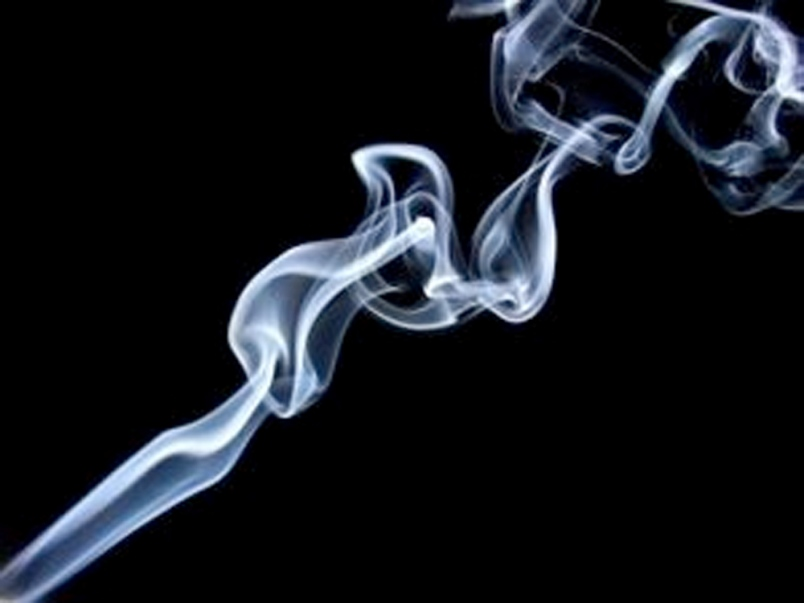
\includegraphics[width=0.5\textwidth]{images/smoke}
%https://www.google.se/search?client=ubuntu&q=cb+edits+smoke+png&tbm=isch&tbs=simg:CAQSlAEJkNL0D0I-7I0aiAELEKjU2AQaBAgVCAAMCxCwjKcIGl8KXQgDEiWoGUHnAegBsQw9sgxAlgawDIYnhSCHJ4okqzemIYgksCiVIKw3GjDJWGns8ZAx_17dvQFajhuRydFWdlJwDNo3VGI7iBUyNViewQZEJmiaYWGUhTUgxQOUgBAwLEI6u_1ggaCgoICAESBLt5JWoM&sa=X&ved=0ahUKEwiit7jKxKXZAhUBiCwKHTapCLQQ2A4IJygB&biw=1916&bih=948
\end{figure}


\subsection{The Boundary Layer}
In the context of fluid dynamics, the boundary layer is the region where a fluid flows close to a solid surface. Imagine a laminar flow close to a solid surface; because of viscosity, the molecules flowing near the surface move slower, and, in the limit, the velocity of the molecules in direct contact with the surface is 0 (this is called the \emph{non-slip condition}). Thus, the velocity of the fluid increases smoothly, continuously and monotonously with the distance from the solid, until it reaches the \emph{free-flow} velocity, after which it stays constant. The region close to the surface, where the fluid moves slower, is called the \emph{boundary layer}, and is the region where the viscosity of the fluid influences its motion. Its height $\delta$ can be defined when the local velocity surpasses a certain threshold, such as 99\% of the free-flow velocity.

The variation of velocity with distance from the surface, $\partial\overline{u}/\partial z$, is called \emph{shear}, and, together with viscosity, determines the materialization of turbulence in the flow. Every layer of fluid is squeezed between a faster moving layer above and a slower moving below; in high shear conditions, this causes high stress on the particles, and prevents them from moving orderly, thus leading to turbulent motion. Figure \ref{fig:bl} shows turbulence forming close to the wall in a canal, where the water flows from right to left. Viscosity and the no-slip condition prevent this phenomenon to arise in a region very close to the solid surface, called the \emph{laminar (or viscuous) sub-layer}, where we still find laminar motion.

The strength of the turbulence is proportional to $u_{rms}=(\overline{u'^2})^{1/2}$, which is, in turn, proportional to the shear. Again, because of the no-slip condition, $u_{rms}$ is zero at $z=0$, increases in the laminar sub-layer, and decreases to 0 at the end of the boundary layer, assuming laminar flow outside of it. Higher free-stream velocity generates higher shear, more turbulence, and a thinner laminar sub-layer. The strength of turbulence can be written in units of velocity, resulting in the \emph{friction velocity}, computed as $u_*=(\tau/\rho)^{1/2}=(\nu\cdot\partial\overline{u}/\partial z)^{1/2}$, where $\tau$ is the shear stress, $\rho$ is the density of the fluid, $\nu=\mu/\rho$ is the kinematic viscosity, and $\mu$ the dynamic viscosity. Therefore, the friction velocity increases with shear and viscosity, and decreases with density; it is proportional to the free-stream velocity and the turbulence strength, and inversely proportional to the height of the laminar sub-layer. Expressing the shear $\tau$ in terms of the horizontal kinematic momentum fluxes $\overline{u'w'}$ and $\overline{v'w'}$, we obtain an equivalent formulation of $u_*$:

\begin{equation}
\label{eq:ustar_momentum}
u_*=\left(\overline{u'w'}^2+\overline{v'w'}^2\right)^{1/4}
\end{equation}

The mean velocity $\overline{u}$ increases linearly within the laminar sub-layer, then logarithmically until the end of the boundary layer, thus the shear decreases further away from the surface. In the logarithmic sub-layer, the velocity is computed as $\overline{u}(z)=u_*(\log z - \log z_0)/\kappa$, where $z_0$ is the characteristic roughness of the surface, and $\kappa$ is the von Karman's constant, whose value is around 0.4 [citation needed]. The characteristic roughness depends on the texture of the surface, and its relationship with the height $\delta_s$ of the laminar sub-layer; if the roughness scale is smaller than $\delta_s$, the logarithmic velocity profile is not affected by the texture, because the laminar sub-layer completely covers the variations on the surface, and we have the so-called smooth turbulent flow. If, on the contrary, the bumps in the surface are larger than $\delta_s$, the laminar sub-layer follow the profile of the surface, and the logarithmic velocity profile is altered depending on the texture, a regime called rough turbulent flow.

\begin{figure}
\caption{Turbulent boundary layer at the edge of a canal; water flows from right to left.}
\label{fig:bl}
\centering
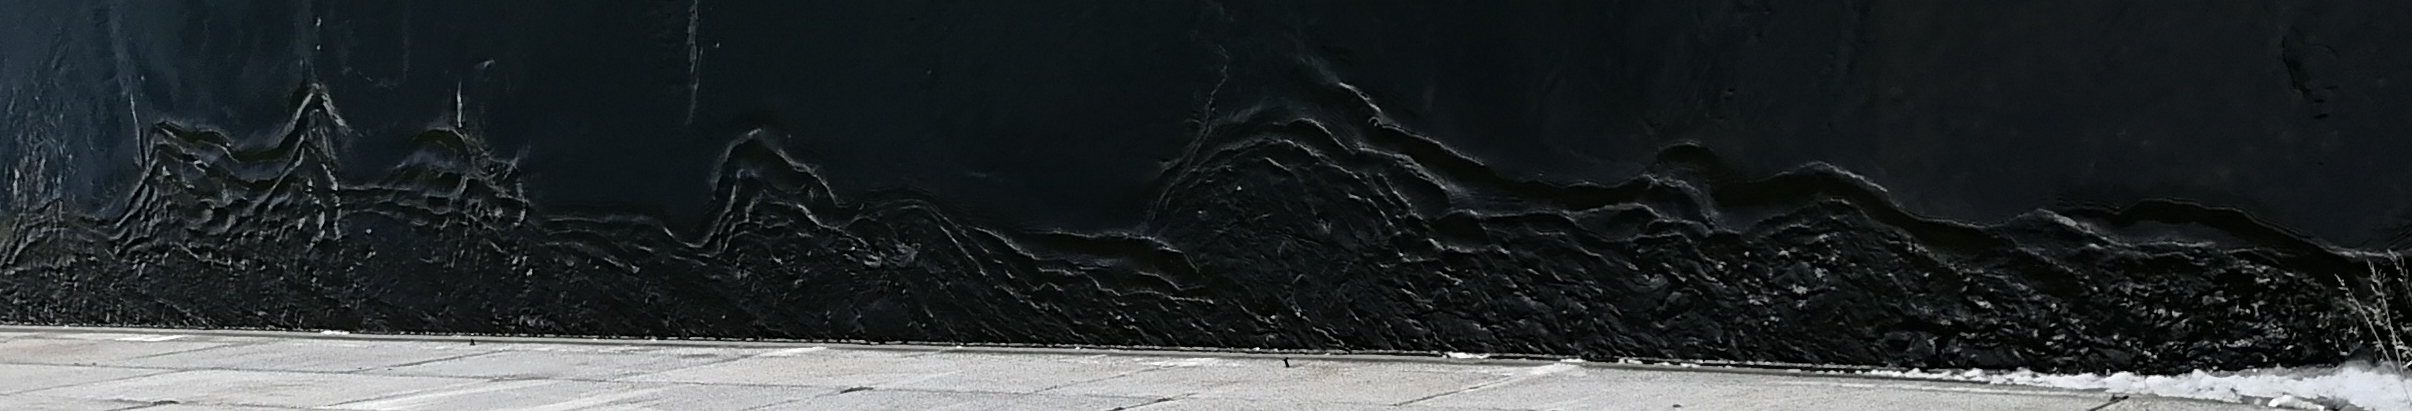
\includegraphics[width=\textwidth]{images/bl}
\end{figure}

\section{The Atmospheric Boundary Layer}
\label{sec:abl}
The atmosphere is composed by air, which is behaves like fluid. Therefore, close to the Earth's surface, in the region called \emph{atmospheric boundary layer}, we find the same effects described in the previous section. Additionally, there are other phenomena that complicate things further, such as the temperature of the surface, which changes widely from day to night and from Summer to Winter, the rotation of the Earth, the varying roughness of the surface, due to cities and vegetation, etc. The effect of the surface on the first few hundred meters of the atmosphere is the main focus of \emph{boundary layer meteorology}. 

The height of the atmospheric boundary layer (hereafter abbreviated as ABL) typically varies between 100 and 1000 meters, highly depending on the conditions, and it is always turbulent. There are two main instabilities driving turbulence in the ABL:

\begin{itemize}
\item Shear instability: caused by shear, the mechanism described in the previous section. This happens at high Reynolds number, and, by using typical values for the ABL, we find $Re$ well above $10^6$.
\item Rayleigh-Bernard (also known as buoyancy driven) instability: is caused by the decrease of potential density\footnote{the potential density is the density that a parcel of air would attain if brought at a standard reference pressure adiabatically, i.e. disallowing exchanges of heat with its surroundings. Potential density is useful to compare densities irrespectively of pressure, i.e. altitude} with height, or, in other words, when warm fluid is below cold fluid; the warm fluid will rise, and the cold fluid will drop, a phenomenon called \emph{convection}. During hot Summer days, the surface is much warmer than the air, thus the air close to the surface will heat and tend to rise.
\end{itemize}

Turbulence has the very important role of transport and mix of air properties, such as heat, moisture, particles, aerosols, etc. This is especially true in \emph{unstable} conditions, when the air moving upwards (e.g. because it is warmer) is less dense than the air moving downwards; when the contrary happens, the ABL is called \emph{stable}.

The ABL can be divided in two main sub-layers: the inner surface layer and the outer Ekmann layer. This distinction is mainly done based on the scale of the dominating turbulent eddies: they are much smaller than the height of the ABL in the surface layer, and of comparable size in the outer layer.

It is very important to have a macroscopic understanding of the turbulent processes in the ABL, because they happen at length and time scales too small to be simulated in global climate models. The process of expressing the result of turbulence as a function of large scale parameters is called parametrization; having realistic models is essential in order to conduct precise simulations of the global climate in the scale of tens or hundreds of years, because errors tend to accumulate and amplificate as the simulation goes on. Other fields that benefit from the study of the ABL are urban meteorology (interested in the dispersion of pollutants), agricultural meteorology (interested in the formation of frost and dew, the temperature of the soil, etc.), aviation (predict fog and strong winds), and so on.

\subsection{Surface Fluxes}
A flux measures the amount of a physical quantity that flows through a surface. In the context of boundary layer meteorology, we are interested in the flows through the surface of earth, because, through them, the surface and the atmosphere exchange energy; these fluxes are thus measured in \si{\watt\per\square\meter}. The main source of energy for the surface is short-wave radiation coming from the sun, and long-wave radiation coming from the atmosphere and the clouds. A small amount of long-wave radiation is emitted from the surface, therefore let the net radiative flux be $R$, positive when the surface gains energy.

The main fluxes by which the surface gains or loses energy to the atmosphere are called the turbulent flux of \emph{sensible heat} $H$, also called kinematic heat flux, and the turbulent flux of \emph{latent heat} $\lambda E$, also called kinematic flux of water vapor/moisture. The difference between the two is that the former causes an actual change of temperature, whereas the latter does not affect temperature\footnote{imagine a pot of boiling water; selecting a higher temperature on the stove will not increase the temperature of water above \SI{100}{\celsius}, but will make it boil faster. The additional heat introduced in the system is dissipated through increased evaporation}. The main causes of sensible heat fluxes are conduction and convection, whereas the main cause of latent heat fluxes is water movement: condensation, evaporation, melting, etc. 

The final flux of interest is the soil heat flux $G$, which is the heat transferred into or out of the deeper layer of the soil and not given back to the atmosphere. These four fluxes are linked by the surface energy balance equation:

$$
R=H+\lambda E+G
$$

which states that the total incoming energy $R$ must be equal to the energy given back to the atmosphere $H+\lambda E$ (not counting long-wave radiation, which is accounted to in $R$) plus the energy absorbed by the surface $G$, assuming the temperature is constant. When the temperature is not constant, one can write a budget equation relating the changes in these quantities.

The turbulent fluxes $H$ and $\lambda E$ are constant in the surface layer. Experimentally, the energy balance is not always achieved \citep{cabauwinsitu} because of the difficulty in measuring fluxes due to eddy correlation being inaccurate.

\subsection{The Turbulence Kinetic Energy Budget}
Kinetic energy is energy stored in form of movement: faster or heavier objects have more kinetic energy than slower or lighter ones. The Reynolds decomposition allows us to decompose the kinetic energy of turbulent flows in two terms: one caused by the mean flow, and one caused by turbulence. This decomposition can be justified by examining the temporal spectrum of kinetic energy, shown in figure \ref{fig:tkespectrum}. Four peaks are visible, corresponding to different sources of kinetic energy: turbulence, day-night cycle, synoptic scale variability, lows and highs passing, and seasons. Importantly, there are few sources of kinetic energy in the 30 minutes to one hour time scale; this so-called spectral gap allows us to separate between turbulence and other sources of fluctuations in the atmosphere.

\begin{figure}
\caption{Long term average of atmospheric kinetic energy at different time-scales. The peaks in the scale of days and months and years are due to the day-night and Summer-Winter cycles, the peaks in the monthly scale are due to baroclinic instability in the mid-latitude westerlies, and the peaks at one minute are due to convection and atmospheric turbulence \citep{tkespectrumsrc,tkespectrumorig}}
\label{fig:tkespectrum}
\centering
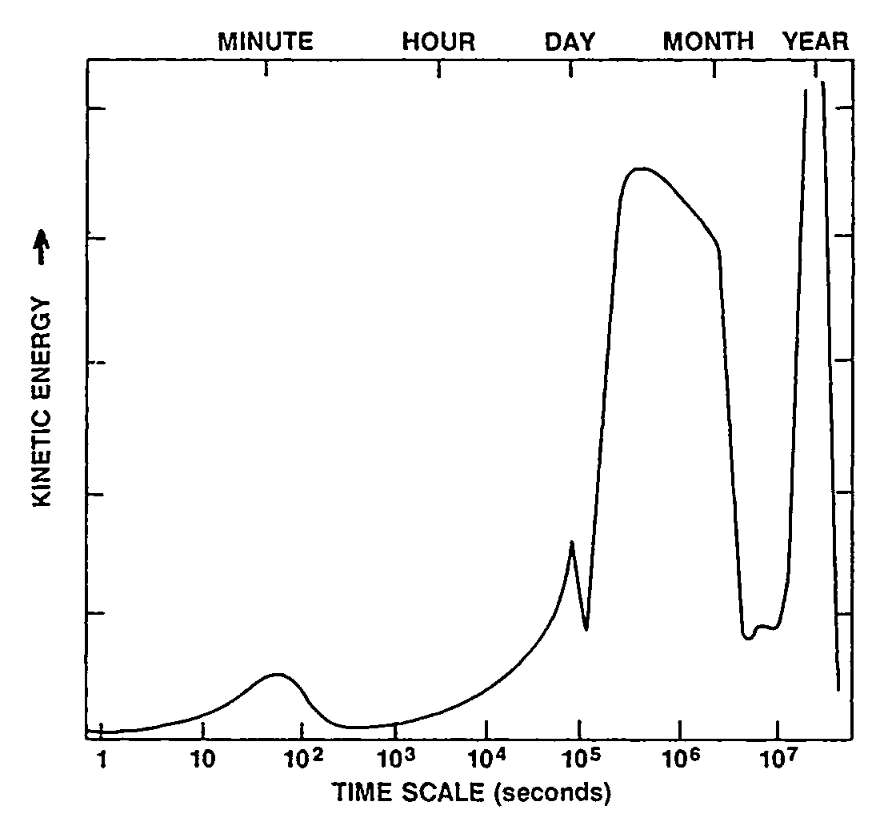
\includegraphics[width=0.5\textwidth]{images/kinetic_energy_spectrum}
\end{figure}

From now on, we will use a coordinate system with the $x$ axis aligned to the average horizontal wind direction, the $y$ axis perpendicular to it, and the $z$ axis pointing away from the surface. Then, we will use the letters $u$, $v$ and $w$ to denote the components of the wind along the axes $x$, $y$ and $z$ respectively; clearly, $\overline{v}=0$. Eddy fluxes can then be described in terms of covariances: let $\theta$ denote the potential temperature\footnote{the potential temperature is final temperature after bringing a parcel of air to a standard pressure adiabatically, i.e. not allowing exchange of temperature with the surroundings. It is a useful mean to compare temperatures irrespectively of pressure, i.e. altitude}, then $\overline{w'\theta'}$ is the turbulent heat flux, i.e. the sensible heat flux in the vertical due to turbulence. Usually the ABL  studied assuming homogeneous horizontal conditions, because they vary on a length scale larger than the height of the ABL. Because of this, the horizontal eddy correlations $\partial\overline{u'a'}/\partial x$ and $\partial\overline{v'a'}/\partial y$ are usually of negligible intensity, and are thus ignored. Note that this is not necessarily true when clouds are involved.

It is important to notice that turbulence is dissipative in nature. Consider a hot Summer day, where air is warmer close to the surface, and a circular eddy moving some air up and some down, so that the average motion is zero. The parcel of air moving up ($w'>0$) ends up being warmer than its surroundings ($\theta'>0$), while the one moving down ($w'<0$) will be colder ($\theta'<0$); the result is a net transport of heat through the eddy: $\overline{w'\theta'}>0$. On the contrary, imagine a cold night, where the air close to the surface is colder; the same eddy would transport a colder parcel of air upwards, and a warmer one downwards. In both cases, the end result would be a net transport of heat without transport of mass. Because of the ??? law, the eddy must lose energy, and thus dissipate over time.

Since turbulence changes over time, we are more interested in the change of kinetic energy, the \emph{turbulent kinetic energy budget}. A full derivation is out of the scope of this work, but its final form \citep{basicatm} can be derived from prime physical principles, resulting in

\begin{equation}
\frac{\partial\overline{{e'}^2}}{\partial t}
=\underbrace{\overline{u'w'}\frac{\partial\overline{u}}{\partial z}}_P
-\underbrace{\frac{g}{T}\overline{w'\theta'}}_B
+\underbrace{\frac{\partial}{\partial z}\frac{\overline{w'{e'}^2}}{2}}_{T_t}
+\underbrace{\frac{1}{\rho}\frac{\partial\overline{p'w'}}{\partial z}}_{T_p}
+\epsilon
\end{equation}

Where ${e'}^2={u'}^2+{v'}^2+{w'}^2$. The $P$ term is the production due to shear, $B$ is the production due to buoyancy, $T_t$ is the turbulent transport of TKE by large-scale eddies, $T_p$ is the transport due to pressure, and $\epsilon$ is molecular dissipation due to viscosity. $P$ and $B$ are the most prominent terms, and the transport terms are close to zero in neutral conditions \citep{basicatm}.

The $P$ term is always positive, as energy is taken from the mean flow to the turbulent one. On the other hand, the contribution from buoyancy can be either positive or negative, depending on the difference of temperature between a parcel of air moved by the turbulence and the surrounding air. When $\overline{w^\prime\theta^\prime}$ is negative, the turbulence is moving cold air upwards and warm air downwards; these parcels of air will try to undo the effect of turbulence, thereby increasing the overall kinetic energy. A similar reasoning goes for when the heat flux is positive.

\subsection{Monin-Obukhov Similarity Theory}
\label{sec:most}
One of the quantities of interest is the momentum flux-profile relationship, computed as follows:

\begin{equation}
\label{eq:phi_m}
\frac{\partial\overline{u}}{\partial z}\frac{\kappa z}{u_*}
\end{equation}

where $\kappa$ is the von Karman constant, which roughly equals 0.4. The profile is expressed by the $\partial\overline{u}/\partial z$ term, and the momentum flux is contained in the friction velocity $u_*$ according its interpretation in equation \ref{eq:ustar_momentum}.

One of the factors to distinguish laminar from turbulent flow is the length scale $L$ of the system. This length scale for the ABL was derived by \cite{mostayyyy}, and forms the basis of the similarity theory. According to this theory, the normalized wind profile of equation \ref{eq:phi_m} can be expressed as an unique \emph{universal} function of $\xi=z/L$, with

\begin{equation}
\label{eq:most_l}
L=-\frac{u_*^3}{\kappa\frac{g}{\theta_v}\frac{Q}{\rho c_\rho}}
=-\frac{u_*^3 T_v}{\kappa g \overline{w'\theta_v}}
\end{equation}

\noindent where

\begin{itemize}
\item $g=\SI{9.81}{\meter\per\square\second}$ the acceleration due to Earth's gravity

\item $\theta_v$ virtual temperature\footnote{potential temperature of dry air if it had the same density as moist air. It allows to use formulas for dry air when the air is not dry.}, obtained as

\begin{equation}
\label{eq:vtemp}
\theta_v=\theta\frac{1+r_v/\epsilon}{1+r_v}=\theta(1+0.61\cdot q)
\end{equation}

Where $\theta$ is the air temperature, $r_v$ is the mixing ratio, $q=r_v/(1+r_v)$ the specific humidity, and $\epsilon$ is the ratio of the gas constants of dry air and water vapor, roughly 0.622.

\item $\rho$ the air density, computed from the pressure $P$ and the specific gas constant for dry air $R=\SI{287.058}{\joule\per\kilo\gram\kelvin}$ as

$$
\rho=\frac{P_0}{RT_v}
$$


\item $c_\rho$ specific heat of dry air, \SI{1005}{\joule\per\kilo\gram\per\kelvin} at \SI{300}{\kelvin}
\item $Q$ the buoyancy flux, approximated by $H+0.07\lambda E$ and measured in \si{\watt\per\square\meter}
\item $\overline{w'\theta_v}=Q/\rho c_\rho$ the flux of virtual potential temperature, measured in \si{\kelvin\meter\per\second}
\item $T_*=-\overline{w'\theta}/u_*$
\end{itemize}

The stability parameter $\xi$ is positive for stable conditions, where wind shear dominates the production of TKE, and negative for unstable conditions, where buoyancy is the main contributor to turbulence. It approaches 0 in the limit of neutral stratification (i.e. $\partial\overline{\theta}/\partial z=0$), because the temperature flux goes to 0 causing $L$ go to infinity.

The universal function must be determined experimentally. This is no easy task, and considerable effort has been devoted to it; one of the greatest difficulties lies in obtaining accurate and unbiased measurements, especially the fluxes. \cite{hogstrom88} is a meta-study that aggregates and improves many previous results, and suggests the following expressions:

\begin{align}
\phi_m(\xi)&=\begin{cases}
\label{eq:phi_m_coeff}
\mathrlap{(1-19.3\xi)^{-1/4}} \hphantom{0.95(1-11.6\xi)^{-1/2}} & -2<\xi<0 \\
1+6\xi & 0<\xi<1\\
\end{cases}
\end{align}


The Monin-Obukhov similarity theory (MOST) is only applicable in the surface layer, at heights much larger than the aerodynamic roughness length, and with $\vert\xi\vert<2$; even under ideal conditions, the predictions of this theory are accurate up to 10-20\% \citep{50years}. Intuitively, when $\vert\xi\vert$ is too large, the eddies do not feel the effect of the surface anymore, and, under very stable stratification ($\xi>>1$), vertical motion is hampered, so the height $z$ does not play a role. Recent attempts \citep{sheba_phim,most_teal,Wilson2008} try to extend, or altogether replace, this similarity theory.

\section{Statistics and Machine Learning}
\label{sec:ml}
The goal of Machine learning is to develop algorithms that allow computers to learn from examples. Learning is intended as the ability of inferring general rules from the available examples, so that new, previously unseen examples can be correctly characterized. The set of samples from which the computer is supposed to learn is called the \emph{training set}, and each sample is a sequence of numbers describing its attributes, or \emph{features}. There are three approaches in machine learning:

\begin{itemize}
\item \emph{Supervised} learning: in this setting, the examples are composed of an input and a desired output, and the goal is to build a model that can correctly predict the output given the input. There are different algorithms depending on the type of output: \emph{regression} algorithms predict continuous output, while \emph{classification} algorithms predict discrete output.

\item \emph{Unsupervised} learning: in this setting, no output is available. The task of the algorithm is to figure out hidden relationships between the samples in the training set, for example whether they form clusters, or there are anomalous samples, or the correlation between features of the examples.

\item \emph{Reinforcement} learning: in this setting, the computer is free to act in an environment and to observe how the environment responds to its actions. Additionally, it receives a \emph{reward} for every action it takes, and the goal of the computer is to learn a sequence of actions that maximizes the received reward. Reinforcement learning is often applied in robotics [citation] and game playing [alphazero citation].
\end{itemize}

A supervised machine learning model uses a set of parameters to compute the output value starting from the input features. The actual parameters values are learned from the training set in a process called \emph{training}. This process is controlled by another set of parameters called hyper-parameters, whose value can be found from the training data as well. Whereas the parameters control the relationship between input and output, hyper-parameters control the "character" of the learning algorithm, such as how eager or conservative it is in learning minute details in the features. Learning too many details can be detrimental, because some differences can be due to noise, rather than actual differences.

The next sections describe the theory of learning, a general technique to estimate the parameters of a regression model, and introduce several machine learning algorithms for regression.

\paragraph{Notation:} Scalars are denoted in \textit{italic}, vectors (always column) and matrices in \textbf{bold}. The training set contains $N$ training samples, indexed by $n$, and each sample is a pair of feature vector $\bm x_n\in\mathbb{R}^D$ and a target value $t_n\in\mathbb{R}$. The feature vectors are grouped in the $N\times D$ matrix $\bm X=\left[\bm x_1\dotsb\bm x_N\right]^\intercal$ and the target values in the $N\times 1$ vector $\bm t=\left[t_1,\ldots,t_n\right]^\intercal$. Models are parametrized by a parameter vector $\bm\theta$ and their output for the feature vector $\bm x_n$ is $f_n=f(\bm x_n;\bm\theta)$. The vector containing both parameters and hyper-parameters is denoted with $\bm\Theta$.

\subsection{Learning Theory}
The goal of supervised learning is to use the training examples $D=(\bm X, \bm t)$, independent and identically distributed according to an unknown distribution $p_{XT}$, to find a good prediction rule $\hat{f}:\mathcal{X}\rightarrow\mathcal{Y}$ among a family of available functions $\mathcal{F}$. In most practical cases, $\mathcal{X}=\mathbb{R}^D$ and $\mathcal{Y}$ is either $\mathbb{R}$ for regression or a subset of $\mathbb{N}$ for classification. The goodness of a prediction rule $f$ is measured through a \emph{loss function} $\ell:\mathcal{Y}\times\mathcal{Y}\rightarrow\mathbb{R}$ that tells, given a target value $t$ and a guess $y=f(x)$, how much the guess is off. The \emph{risk} of an estimator $f$ is simply its expected loss:

\begin{equation}
R(f)=\mathbb{E}_{(x,t)\sim p_{XT}}\left[\ell(f(x),t) \vert f \right]
\end{equation}

The ideal situation is to find the estimator $f^*$ that has the lowest risk; unfortunately this is not possible, because the distribution $p_{XT}$ is unknown. Since the training data is a sample from this distribution, we can compute the \emph{empirical risk} of $f$ on this set of examples instead:

\begin{equation}
\hat{R}(f)=\mathbb{E}_{(x,t)\sim D}\left[\ell(f(x),t)\vert f\right]=\frac{1}{N}\sum_{n=1}^N \ell(f(x_n),t_n)
\end{equation}

We can now use the empirical risk as a surrogate for the true risk, selecting the estimator

\begin{equation}
\hat{f}=\argmin_{f\in\mathcal{F}}\hat{R}(f)
\end{equation}

\noindent as our best guess. This procedure is called \emph{empirical risk minimization}. Note that $\hat{f}$ is a random function, because it depends on $D$, which is a random variable. An interesting question to ask is how good $\hat{f}$ actually is, or, in other words, what is its expected true risk $\mathbb{E}[R(\hat{f})]$ and how it compares to the lowest attainable risk $R(f^*)$. This latter quantity can be decomposed as

\begin{equation}
\mathbb{E}[R(\hat{f})]-R(f^*)=
\left(\mathbb{E}[R(\hat{f})]-\inf_{f\in\mathcal{F}} R(f)\right)
+\left(\inf_{f\in\mathcal{F}} R(f)-R(f^*)\right)
\end{equation}

Where the first term is the \emph{estimation} error incurred by not selecting the best possible estimator in $\mathcal{F}$, and the second term is the \emph{approximation} error caused by searching a good estimator in $\mathcal{F}$. They usually have opposite behavior:

\begin{itemize}
\item the estimation error is high when $\mathcal{F}$ is too complex for the data at hand, where complexity refers to the range of phenomena that can be accurately modeled by these functions. In other words, $\mathcal{F}$ contains many valid explanations that are equally good on the training set (they have low empirical risk $\hat{R}$), but are not accurate models of the underlying phenomenon $p_{XT}$, i.e. they do not generalize well (they have high risk $R$);
\item the approximation error is high when $\mathcal{F}$ cannot adequately model the phenomenon that we are trying to describe, i.e. when it does not contain any good explanation for it.
\end{itemize}

This decomposition is often referred to as the \emph{bias-variance decomposition}, where bias and variance refer to, respectively, approximation and estimation error.

The fundamental problem is to find a class of functions that is powerful enough to model $p_{XT}$, but not too powerful so as to contain too many good explanations, because we would not be able to choose. Equivalently, we want to find a good model, one that can explain the data we have, and generalize to new examples. This problem is known as \emph{model selection}, and is important to distinguish between model selection for \emph{identification}, and model selection for \emph{estimation}. In the former case, the goal is to obtain a model and its parameters, to be used on new prediction problems, whereas the goal of the latter is to obtain a realistic estimate of the performance that can be obtained on new data. This problem can be approached in two ways: by directly estimating approximation and estimation errors using hold-out sets, or by penalizing complex models in order to favor simpler explanations, even though they might have slightly higher empirical risk. The next sections describe these two approaches.


\subsection{Cross Validation}
\label{sec:cv}
The idea behind hold-out methods is to partition the available data in two smaller sets $D_T$ and $D_V$, usually of size 2/3 and 1/3 of the total, and use the \emph{training} set $D_T$ to choose $\hat{f}$ and $D_V$ to estimate its risk. Since $D$ is assumed to be a representative sample from $p_{XT}$, if the two partitions contain independent and identically distributed samples, the empirical risk on the \emph{validation set} $D_V$ can give us a glimpse on the generalization power of $\hat{f}$. This is because the validation set contains new samples that were not used to choose $\hat{f}$, thus the empirical risk on this set is an unbiased estimate of the true risk of the discovered model. This allows us not only to be confident about the performance of the estimator on unseen data, but also to compare different estimators. The problem of a single hold-out set is the variance of its estimate of the risk, which depends on the size of the validation set. This means that we are faced with a trade-off: use a lot of data to select a good estimator, but have high uncertainty in its estimated performance, or use less data and select a less powerful estimator, but have a more accurate picture of its performance.

The solution to this problem is to repeatedly perform this partitioning procedure so as to obtain many estimates of the risk, each on a different subset of validation samples, and average these results together. This can be done in a number of different ways:

\begin{itemize}
\item in random subsampling, the procedure above is simply repeated many times, by using two thirds random examples for training, and the remaining one third for validation;
\item In bootstrapping \citep{bootstrap}, the training set is created by taking $N=\vert D\vert$ examples \emph{with replacement} from $D$, and using the remaining examples for validation. This means that the validation set contains on average approximately 36.8\% of the samples in $D$, and the training set the remaining 63.2\%, with many duplicates;
\item In $k$-fold cross validation \citep{kfold}, $D$ is partitioned in $k$ subsets, and each of them is used in turn as validation set, while the others are used for training. This produces $k$ estimates of the true risk, coming from the $k$ subsets.
\end{itemize}


\begin{algorithm}
\caption{Nested cross validation with random hyper-parameter search.}
\label{alg:nested_cv}


\algnewcommand\algorithmicinput{\textbf{Input:}}
\algnewcommand\Input{\item[\algorithmicinput]}

\algnewcommand\algorithmicoutput{\textbf{Output:}}
\algnewcommand\Output{\item[\algorithmicoutput]}

\begin{algorithmic}
\Input \\
\begin{itemize}
\item[$D$] Dataset
\item[$K_O$] Number of outer folds
\item[$K_I$] Number of inner folds
\item[$R$] Number of random combinations to try
\item[$model$] Model to train
\item[$distrs$] Distribution of each hyper-parameter
\end{itemize} \\
\Output Summary statistics computed on each outer validation fold \\

\For{$k_o\gets 1\ldots K_O$}\Comment{Outer $K_O$-fold cross validation}
	\State{Generate $k_o$-th outer fold $(D^o_T,D^o_V)$ from the dataset $D$}
	\State{$best\_mse\gets\inf$}
	\State{$best\_params\gets\bot$}
	\For{$r\gets 1\ldots R$}\Comment{Find best hyper-parameters on $D^o_T$}
		\State{$params\gets$ a random hyper-parameter combination from $distrs$}
		\State{$params\_mse\gets 0$}
		\For{$k_i\gets 1\ldots K_I$}\Comment{Evaluate $params$ with $K_I$-fold CV}
			\State{Generate $k_i$-th inner fold $(D^i_T,D^i_V)$ from $D^o_T$}
			\State{$model\gets$ a new instance of the model with parameters $params$}
			\State{Train $model$ on $D^i_T$}
			\State{$mse\gets$ result of the evaluation of $model$ on $D^i_V$}
			\State{$params\_mse\gets params\_mse+mse$}
		\EndFor

		\If{$params\_mse<best\_mse$}\Comment{MSE comparison on $K_i$-fold CV result}
			\State{$best\_mse\gets params\_mse$}
			\State{$best\_params\gets params$}
		\EndIf		
	\EndFor

	\State{$model\gets$ a new instance of the model with parameters $best\_params$}
	\State{Train $model$ on $D^o_T$}
	\State{Evaluate $model$ on $D^o_V$ and compute evaluation metrics}
\EndFor
\State{Compute summary of the metrics obtained in the outer loop}
\end{algorithmic}
\end{algorithm}

Regardless of the method used, the final estimate of the performance is the average of the estimates obtained from the individual trials. Every method has different properties regarding both the bias and the variance of the estimates, and there is considerable controversy on which method should be used in which situation. For example, \cite{cv_bootstrap} recommends using 10-fold CV for comparing models, because, although its estimate of the performance is biased, it has lower variance compared to bootstrapping; however, \cite{no_unbiased_cv} show that it is not possible to obtain an universal unbiased estimate of the variance of $k$-fold CV. \cite{cvmyths} further discusses this issue, and debunks some myths and commonly held misconceptions about CV, including the belief, consequent \cite{cv_bootstrap}, that 10-fold cross validation is always the best choice. Generally, there is a tradeoff in choosing the value of $k$, as high values yield estimates with lower bias, but higher variance \citep{cv_survey}, and are more computationally intensive.

Cross validation can be used to perform two distinct tasks: \emph{estimation} and \emph{identification}. The goal of the former is to accurately estimate the best performance attainable on a prediction problem, whereas the goal of the latter is to identify the parameters and hyper-parameters that give rise to the best possible estimators. Consequently, when the goal is estimation we want to eliminate bias, whereas in identification we need low variance. Estimation is best performed with nested CV\citep{nested_cv_stone,nested_cv_varma}, in which there is an inner CV loop done on every training fold of the outer CV loop. This procedure is formalized in algorithm \ref{alg:nested_cv}, where random hyper-parameter search \citep{random_search} is used in the inner CV loop to find good values for the hyper-parameters. \cite{cv_pitfalls} advocates for repeating nested CV, since plain nested CV produces estimates with fairly high variance, but the computational cost of such procedure can be prohibitively high.


\subsection{Parameter Estimation for Regression}
\label{sec:regression_fit}

In this section, we describe a general framework, rooted in Bayesian statistics, for estimating the parameters of a regression model, while controlling overfitting. An advantage of Bayesian methods is that they offer a sound theoretical foundation for model selection, without requiring repeated experiments to choose among candidate models, although this mathematical rigor is not free from practical difficulties \citep{bayesian_model_selection, practical_bayesian_model_selection}.

A common assumption in the regression setting is that the observations are corrupted by additive Gaussian white noise, i.e. $t_n=y_n+\epsilon_n$, where $y_n$ is the "true" value, and $\epsilon_n\sim\mathcal{N}(0,\beta^{-1})$ is the noise. Let $f_n=f(\bm x_n;\bm{\theta})$ be the model's prediction for the sample $\bm x_n$, then we can write the probability of observing $t_n$, assuming that $f_n=y_n$, as:

\begin{equation}
\label{eq:model_pred_distrib}
p(t_n\vert \bm{x_n},\bm\Theta)=\mathcal{N}(t_n\vert f(\bm{x_n};\bm\theta),\beta^{-1})
\end{equation}

This probability is called \emph{likelihood} of the observation $t_n$, under the model $f(\cdot;\cdot)$ with parameters $\bm{\theta}$. Since the training data is assumed to be independent and identically distributed, the likelihood of the whole training set is

\begin{equation}
\label{eq:likelihood}
p(\bm{t}\vert\bm{X}, \bm\Theta)=\prod_{n=1}^N  \mathcal{N}(t_n\vert f(\bm{x_n};\bm\theta),\beta^{-1})
\end{equation}

And the predicted value $t$ for a new sample $\bm x$ is distributed as

\begin{equation}
p(t\vert \bm x, \bm X, \bm t)=\int
p(t\vert\bm x,\bm\Theta)\cdot p(\bm\Theta\vert \bm t, \bm X)\ \text{d}\bm\Theta 
\end{equation}

In practice, it is not feasible to compute this integral, and its value is dominated by the values of $\bm\Theta$ close to the one that maximizes equation \ref{eq:likelihood} anyways; this is the gist of \emph{maximum likelihood estimation} (MLE). Note that, since the goal is to predict $y_n$, there is a high probability that the "true" parameters would \emph{not} be the ones with maximum likelihood. When a model learns the noise in the training data, it cannot generalize well to new, unseen data, because the noise is random. This situation is known as \emph{overfitting}, and tends to happen when the model is too complex relative to the amount of data available for training, and is related to high estimation error mentioned previously.

The risk of overfitting can be reduced with a number of \emph{regularization} strategies. A widely used strategy consists in including a prior distribution on the parameters of the model, and maximizing their posterior distribution, computed using Bayes theorem:


\begin{align}
\begin{split}
\label{eq:map}
p(\bm\Theta\vert\bm t, \bm X)&=\frac{p(\bm X, \bm t\vert\bm\Theta)\cdot p(\bm\Theta)}{p(\bm X, \bm t)}\\
&\propto p(\bm t\vert \bm X,\bm\Theta)\cdot p(\bm X\vert\bm\Theta)\cdot p(\bm\Theta)\\
&\propto p(\bm t\vert \bm X,\bm\Theta)\cdot p(\bm\Theta)
\end{split}
\end{align}


\noindent where we removed $p(\bm X,\bm t)$ and $p(\bm X\vert\bm\Theta)=p(\bm X)$ because they are constant for a given dataset, and we are not interested in the exact probability, but where it reaches its maximum value. This parameter estimation procedure is called \emph{maximum a posteriori} (MAP). Two commonly used prior distributions are the multivariate Laplace and the multivariate Normal, leading respectively to L1 and L2 regularization, when centered and symmetrical/spherical. Note that MAP reduces to MLE when we assume an uniform prior $p(\bm\Theta)$.

The maximization of the posterior can be done conveniently by maximizing its logarithm; this gives expressions that are easier to handle analytically, and give less numerical problems when computed. The MAP problem can be formulated as follows:

\begin{equation}
\bm\Theta^*=\argmax_{\bm\Theta}\ \log p(\bm t\vert\bm X,\bm\Theta)+\log p(\bm\Theta)
\end{equation}


If we assume a Gaussian likelihood like the one in equation \ref{eq:likelihood}, and a spherical Gaussian prior distribution $p(\bm\theta)=\mathcal{N}(\bm 0, \lambda\bm I)$, the MAP estimation of equation \ref{eq:map} becomes, after removing unnecessary constant terms,

\begin{equation}
\label{eq:least_squares}
\bm\theta^*=\argmin_{\bm\theta}\ L(\bm\theta)=\argmin_{\bm\theta}\sum_{n=1}^N\left( f(\bm x_n,\theta)-t_n\right)^2+\lambda\bm\theta^\intercal\bm\theta
\end{equation}

\noindent where $L$ is the \emph{loss function}, in this case the sum-of-squares error. It is customary to use the mean squared error instead of the sum of squares because it results in smaller numbers and is readily interpreted; being only a constant factor away from \ref{eq:least_squares}, it does not transcend the essence of MAP estimation. The parameter $\beta$ can be estimated as well in a similar way, if necessary, and a fully Bayesian treatment allows to estimate $\lambda$, too. Depending on the model $f(\bm x_n,\bm\theta)$, \ref{eq:least_squares} can be solved analytically to yield a closed-form solution for $\bm\theta$.
 
When this is not possible, iterative optimization methods are employed. A widely used approach is called \emph{gradient descent}: the gradient of a function computed at a given location "points" to the steepest direction where the function's value increases. By repeatedly following the gradient, it is possible to reach a local maximum, and, in the opposite direction, a local minimum:

\begin{equation}
\bm\theta_{n+1}:=\bm\theta_n-\eta\cdot\nabla f(\bm x_n)
\end{equation}

The series $\bm\theta_1,\ldots,\bm\theta_n$ is guaranteed to converge to the local optimum at a rate of $O(n^{-1})$ if certain conditions are met \citep{gd_convergence}. \cite{numopt} describes more advanced optimization techniques that use the gradient and, possibly, the Hessian, such as Newton's. The gradient of $L(\bm\theta)$ is

\begin{equation}
\label{eq:least_squares_gradient}
\nabla_{\bm\theta}\log p(\bm\theta\vert\bm t,\bm X)
=2\sum_{n=1}^N \big(f(\bm x_n;\theta)-\bm t_n\big)\cdot\nabla_{\bm\theta}f(\bm x_n;\theta) + 2\lambda\bm\theta
\end{equation}

\noindent and its Hessian is

\begin{equation}
\label{eq:least_squares_hessian}
\nabla^2_{\bm\theta}\log p(\bm\theta\vert\bm t,\bm X)=2\sum_{n=1}^{N}\bigg[
\big(\nabla_{\bm\theta} f(\bm x_n;\bm\theta)\big)
\big(\nabla_{\bm\theta} f(\bm x_n;\bm\theta)\big)^\intercal
+\big(f(\bm x_n;\bm\theta)-t_n\big)\nabla^2_{\bm\theta}f(\bm x_n;\theta)\bigg]+2\lambda\bm I
\end{equation}

In some cases, the gradient and the Hessian can be approximated using a random subset of the training set, and, in extreme cases, a single sample. These variants are called \emph{minibatch} gradient descent and \emph{stochastic} gradient descent respectively. They both compute a noisy approximation to the true gradient, which can actually improve convergence and generalization of high-dimensional, non-convex loss functions such as those found in deep learning \citep{sgd_noise, bayesian_sgd}. Vanilla gradient descent can be greatly improved with a number of techniques, such as momentum \citep{gd_momentum}, adaptive learning rate \citep{adagrad, adadelta, adam}, and so on, see \cite{gd_overview} for an overview. 

\subsection{Hyper-parameter Optimization}
The previous section discussed some methods to find the best parameters for a model. In practice, though, finding good values for the hyper-parameters is often as important as fitting the model, since these hyper-parameters control the learning process itself.

A simple way to approach this problem is to choose some possible values for each hyper-parameter, try all the possible combinations, and pick the one that works best. Alternatively, one can sample each hyper-parameter from a probability distribution, and try many random combinations of values; \cite{random_search} showed that this latter method is surprisingly effective at this task, and scales much better than the former. Unfortunately, this procedure can overfit, too, so it has to be paired with some resampling technique such as cross validation. The procedure is simply to test every hyper-parameter combination on every fold, so that 50 combinations tested with 10-fold cross validation require to fit the model 500 times.

More sophisticated techniques treat hyper-parameter optimization as a regression problem, and use supervised machine learning to predict the performance of a given hyper-parameter combination, and to guide the search accordingly \citep{hyperopt}. Clearly, one should use models that are not sensitive to their own hyper-parameter setting, or the problem is just moved! For this reason, popular algorithms that are used for this are evolutionary algorithms and Bayesian non-parametric models.

\subsection{Ridge Regression}
\label{sec:ridge}
A linear regression model has the form $f(\bm x_n;\bm\theta)=\bm\theta^\intercal\bm x_n$; ridge regression is simply L2-regularized linear regression. This model is simple enough that the solution for equation \ref{eq:least_squares} can be found analytically in closed form:

\begin{equation}
\label{eq:ridge_solution}
\bm\theta^*=(\bm X^\intercal\bm X+\lambda\bm I)^{-1}\bm X^\intercal\bm t
\end{equation}

Notice that the term \emph{linear} in linear regression refers to linearity with respect to the parameters, not the features. In fact, new features can be added through the use of a possibly non-linear feature mapping $\phi:\mathbb{R}^D\rightarrow\mathbb{R}^M$, such that $\bm x^\prime_n=\phi(\bm x_n)^\intercal=\left[\phi_1(\bm x_n),\ldots,\phi_M(\bm x_n)\right]^\intercal$. Then, the model parameters can be fitted to the augmented training set $\bm\Phi=\bm X^\prime$, where $\bm\Phi$ is called the \emph{design matrix}. A typical feature added is a bias $\phi_1(\bm x)=1$.

\subsection{k-Nearest Neighbors}
The k-nearest neighbor model \cite{knn} predicts a value for a sample $\bm x$ by averaging the target values of the $K$ training samples that are closest to $\bm x$, possibly weighted by distance or some other metric. Let $\bm t_{(1)},\ldots,\bm t_{(K)}$ be the target values of the $K$ training samples closest to $\bm x$ according to a distance metric $d:\mathbb{R}^D\rightarrow\mathbb{R}$, then we have

\begin{equation}
f(\bm x)=\sum_{k=1}^K w_{(k)}\cdot\bm t_{(k)}
\end{equation}


Note that the k-nearest neighbors algorithm does not have parameters, only hyper\hyp{}parameters: $K$ itself, the distance function, and the weighting scheme. Typical distance functions are the Manhattan distance $d(\bm u,\bm v)=\sum_{d=1}^D\vert u_d-v_d\vert$ and the squared Euclidean distance $d(\bm u,\bm v)=\sum_{d=1}^D(u_d-v_d)^2$, and typical weights are uniform $w_{(k)}=1/K$ and based on distance $w_{(k)}=d(\bm x,\bm x_{(k)})/\sum_{k^\prime=1}^K d(\bm x,\bm x_{(k^\prime)})$.

\subsection{Gradient Boosted Trees}
Gradient boosting \citep{gradientboosting} is a general method of combining several weak predictors in order to obtain a stronger one. The final prediction for a sample is obtained as a weighted average of the predictions of the individual models:

\begin{equation}
\label{eq:gboost}
f_M(\bm x)=\sum_{m=1}^M \beta_m h(\bm x;\bm\theta_m)
\end{equation}

Each model parameters $\bm\theta_m$ and the weight $\beta_m$ are found by improving the predictions of $f_{m-1}$:

\begin{equation}
\label{eq:gboostjoint}
(\beta_m, \bm\theta_m)=\argmin_{\bm\theta,\beta}\sum_{n=1}^N L\left(
t_n, f_{m-1}(\bm x_n)+\beta h(\bm x_n,\bm\theta)
\right)
\end{equation}

\noindent where $L$ is the loss function, such as the squared error introduced previously. This optimization problem can be challenging, depending on the specific form of $h$ and $L$. Actually, equation \ref{eq:gboostjoint} is equivalent to gradient descent in function space\footnote{this means that you actually modify the function itself, not its parameters, as we did in section \ref{sec:regression_fit}. This is true provided that the parametric function $h$ is able to represent the gradient} \citep{boostinggd,greedyboosting}. This gradient can be computed explicitly on the $N$ training points, but we do not know how to compute it on the other points that are not in the training set\footnote{this is the essence of gradient descent in function space, since a function is defined for every point (at least the functions we consider in Machine Learning are)}. The fundamental idea is to find a model that can predict this gradient, by training it on the dataset. This model is exactly $h$ with parameters $\bm\theta_m$:

\begin{equation}
\label{eq:gbtheta}
\bm\theta_m=\argmin_{\bm\theta}\sum_{n=1}^N \left[
-g_m(\bm x_n)-h(\bm x_n,\bm\theta)
\right]^2
\end{equation}

\noindent with $g_m$ being the gradient of $L$ with respect to $f_{m-1}$:

\begin{equation}
\label{eq:gbgrad}
g_m(\bm x_n)=\frac{\partial L(t_n,f_{m-1}(\bm x_n))}{\partial f_{m-1}(\bm x_n)}
\end{equation}

Then, the step size $\beta_m$ is obtained by line search, i.e. minimizing the loss function in the direction of the gradient:

\begin{equation}
\label{eq:gbbeta}
\beta_m=\argmin_{\beta}\sum_{n=1}^N L(t_n, \beta h(\bm x_n,\theta_m))
\end{equation}

This is now a tractable problem, since \ref{eq:gbgrad} can be computed easily, and both \ref{eq:gbtheta} and \ref{eq:gbbeta} are simple regression problems.

If $L(y_n,t_n)=(y_n-t_n)^2/2$, we have that $-g_m(\bm x_n)=f_{m-1}(\bm x_n)-t_n$, or, in other words, we are creating a new model by counteracting the errors of the current model! Other popular loss functions are the least absolute deviation, $L(y_n,t_n)=\vert y_n-t_n\vert$, in which case $-g_m=sign(t_n-f_{m-1}(\bm x_n))$, and the Huber loss:

\begin{equation}
\label{eq:huberloss}
L_\delta(t_n,y_n)=\begin{cases}
\frac{1}{2}(y_n-t_n)^2 & \vert y_n-t_n \vert \leq \delta \\
\delta(\vert y_n-t_n\vert-\frac{1}{2}\delta) & \vert y_n-t_n \vert > \delta \\
\end{cases}
\end{equation}

\noindent which is robust to outliers as least absolute deviation, but does not penalize small errors too much, like least squares. In this case,

\begin{equation}
-g_m(\bm x_n)=\begin{cases}
t_n-y_n & \vert t_n-y_n\vert\leq\delta \\
\delta\cdot sign(t_n-y_n) & \vert t_n-y_n\vert>\delta
\end{cases}
\end{equation}

In summary, the gradient boosting algorithm starts with a simple prediction $f_0$, such as the average of the true values, builds a model of the form in equation \ref{eq:gboost} by iteratively applying equations \ref{eq:gbtheta} and \ref{eq:gbbeta}.

A popular choice is to use decision trees for $h$. Often, an additional \emph{learning rate} parameter is introduced to shrink the $\beta$ coefficients. Other hyper-parameters for this algorithm are $M$, the the number of boosting steps to perform, the number of examples to use to compute equations \ref{eq:gbtheta} and \ref{eq:gbbeta}, the number of features used to build the trees, their maximum depth, and so on.

A popular extension to vanilla gradient boosting is \emph{extreme gradient boosting} \citep{xgboost}, which essentially adds both L1 and L2 regularization to the loss function, helping to reduce overfitting, and provides better scalability.

\subsection{Gaussian Processes}
A Gaussian Process (GP) is a collection of an infinite number of random variables, such that the joint distribution of any finite subset of them is Gaussian. Intuitively, this allows us to define a distribution over functions, since there is a random variable for every point of the input space. We can sample a function out of a GP by obtaining the random variables at the points of interest; their distribution is a (multivariate) Gaussian, with a certain mean and covariance, and a sample from this distribution contains the values of the sampled function at the points we queried. This process is expressed as follows:

\begin{equation}
\label{eq:gp_marg}
p(\bm y\vert\bm X)=\int p(\bm y\vert \bm f)p(\bm f\vert\bm X)\text{d}f
\end{equation}

Where $\bm X$ are the query points, $\bm f$ a function sampled from the GP, and $\bm y$ the value of the function at the query points. By definition of GP, all the distributions in equation \ref{eq:gp_marg} are Gaussian, since the Gaussian distribution is self-conjugate\footnote{referring to equation \ref{eq:map}, the prior is said to be conjugate to the likelihood if the posterior has the same algebraic form of the prior; the Gaussian distribution is self-conjugate, because a Gaussian prior with a Gaussian likelihood results in a Gaussian posterior. Conjugate distributions are mostly used for algebraic convenience.}. Simplistically, a GP is just a way of computing the mean and covariance of $\bm f$ given $\bm X$, i.e. $p(\bm f\vert\bm X)$; $\bm f$ is then a multivariate Gaussian, which we can manipulate as usual.

Consider the setting of ridge regression described in section \ref{sec:ridge}, where $\bm y=f(\bm X;\bm\theta)=\bm\Phi\bm\theta$, with $\bm\Phi$ being the design matrix. Recall that in section \ref{sec:regression_fit} we introduced the Maximum A Posteriori estimation method by using a prior distribution on the model parameters $\bm\theta$; this makes $\bm y$ a random variable itself. If we use an isotropic Gaussian for $\bm\theta$, we have that the distribution of $\bm y$ is again Gaussian with mean

\begin{equation}
\mathbb{E}[\bm y]=\mathbb{E}[\bm\Phi\bm\theta]=\bm\Phi\mathbb{E}[\bm\theta]=\bm 0
\end{equation}

\noindent and covariance

\begin{equation}
\text{cov}[\bm y]=\mathbb{E}[\bm y\bm y^\intercal]
=\bm\Phi^\intercal\mathbb{E}[\bm\theta^\intercal\bm\theta]\bm\Phi
=\alpha^{-1}\bm\Phi^\intercal\bm\Phi=\bm K
\end{equation}

Where $\alpha$ is the precision of the prior on $\bm\theta$. This is a simple GP with zero mean, and whose covariance between any two points can be computed as the dot product of their features.

In general, we can use any function $k$ to compute the covariance between two input points, as long as the resulting matrix $\bm K$, with $K_{ij}=k(\bm x_i,\bm x_j)$ is symmetric and positive semi-definite\footnote{this means that $\bm K^\intercal=\bm K$ and $\bm v^\intercal\bm K\bm v\geq 0$ for any $\bm X$ (used to compute $\bm K$) and $\bm v$. This condition is necessary for $\bm K$ to be a valid covariance matrix}. We call any such function  \emph{kernel}, a function $k:\mathbb{R}^d\times\mathbb{R}^d\rightarrow\mathbb{R}$ that, intuitively, expresses the similarity of any two input vectors. Mercer's theorem guarantees that for every symmetric positive-definite kernel there exists a basis function $\phi$, such that the kernel corresponds to the dot product in the space generated by $\phi$. In practice, this means that we do not have to explicitly define $\phi$, and that we can even use basis functions that create an infinite dimensional space. Commonly used kernels are the radial basis function kernel:

\begin{equation}
k(\bm x, \bm x^\prime)=\exp\left(-\frac{\Vert\bm x-\bm x^\prime\Vert^2}{2\sigma^2}\right)
\end{equation}

\noindent where $\Vert\bm x-\bm x^\prime\Vert^2=\sum_d(\bm x_d-\bm x_d^\prime)^2$ is the squared Euclidean distance, and which incidentally corresponds to an infinite dimentional basis function, and the linear kernel:

\begin{equation}
k(\bm x, \bm x^\prime)=\sigma^2\bm x^\intercal\bm x^\prime
\end{equation}

Furthermore, certain operations on a kernel generate another valid kernel, and kernels can be combined in certain ways to produce new kernels. For example, the product of a kernel with a positive constant is a valid kernel, the sum and product of two kernels are valid kernels, etc. Generally, a kernel can have parameters, which we denote, as usual, as $\bm\theta$.

In order to use a Gaussian Process for inference (in the regression setting), we need to compute the predictive distribution $p(\bm y\vert\bm X, \bm t, \bm X^*,\bm\theta) $, where $\bm X^*$ is the matrix containing the vectors for which we want to predict the value $\bm y$. We know that the predictive distribution is Gaussian, therefore its mean $\bm\mu_{\bm y}$ and covariance $\bm\Sigma_{\bm y}$ can be obtained relatively easily, resulting in:

\begin{equation}
\label{eq:gp_pred_mean}
\bm\mu_{\bm y}=K_{\bm\theta}(\bm X^*,\bm X) K_{\bm\theta}(\bm X,\bm X)^{-1}\bm t
\end{equation}

\begin{equation}
\bm\Sigma_{\bm y}=K_{\bm\theta}(\bm X^*,\bm X^*)-K_{\bm\theta}(\bm X^*,\bm X)^\intercal K_{\bm\theta}(\bm X, \bm X)^{-1}K_{\bm\theta}(\bm X,\bm X^*)
\end{equation}

\noindent where $K_{\bm\theta}(\bm A,\bm B)$ is a matrix whose $(i,j)$ cell equals to $k(A_i,B_j;\bm\theta)$. From these formulas, note that in order to use GPs, one needs to remember the kernel matrix, of size $N^2$ and invert it, an operation which has a computational complexity of $O(N^3)$; this makes GPs, and any method based on kernels, hard to scale up.

Up until now, we assumed the kernel was fixed, and treated $\bm\theta$ as hyper-parameters. We could use one of the cross validation methods described in section \ref{sec:cv} to find their values, but the Bayesian framework that we used to derive GP allows us to find $\bm\theta$, too, by maximizing $\log p(\bm t\vert\bm X,\bm\theta)$\footnote{obtained as in equation \ref{eq:gp_marg}, usually called log-marginal-likelihood, since we marginalized $\bm f$} with respect to $\bm\theta$. This function often has many local maxima, and is usually optimized by means of gradient descent.

Finally, the derivative of a GP is itself a GP, whose mean is obtained simply by deriving equation \ref{eq:gp_pred_mean} \citep{gp_diff}:

\begin{equation}
\label{eq:gp_gradient}
\frac{\partial\bm y}{\partial\bm X_*}=\frac{\partial K_{\bm\theta}(\bm X_*,\bm X)}{\partial\bm X_*}K_{\bm\theta}(\bm X,\bm X)^{-1}\bm t
\end{equation}

We invite the reader to refer to \cite[Chapter~6]{bishop} for an in-depth treatment of kernel methods, including Gaussian Processes.


\subsection{Robust Effect Size}
\label{sec:effect_size}
The effect size is a statistic used to compare the means of two populations, usually called \emph{control} and \emph{treatment}, that is computed as the standardized difference of the means:

\begin{equation}
\label{eq:base_es}
\delta=\frac{\mu_t-\mu_c}{\sigma}
\end{equation}

\noindent where $\mu_t$ and $\mu_c$ are the means of the treatment and control groups respectively, and $\sigma$ is a normalizer that can be computed in essentially three ways: when the standard deviations of the control and treatment populations can be assumed to be equal, then $\sigma$ should be the pooled standard deviation\footnote{the average standard deviation of the control and treatment groups, weighted by the degrees of freedom (one less than the number of observations) of each group}, otherwise it should be the standard deviation of either the control or treatment group. Generally, the effect size is computed to be positive when the treatment group represent an improvement over the control group.

Recently, there is a departure from the standard procedure of reporting p-values, test statistics and critical values resulting from hypothesis testing towards reporting effect sizes and their confidence intervals, in addition or in alternative to the usual statistics, see for example \cite{apa} and \cite{aera}.  However, effect sizes can be as misleading as significance testing when the assumptions underlying its expression are violated; commonly used effect size measures, such as Cohen's $d$ [citation], assume both populations are normally distributed and have the same standard deviation\footnote{a property called \emph{homoscedasticity} (contrary: heteroscedasticity)}. Alternatives that do not assume equal standard deviation exist \citep{es1,es2,es3}, but they all require normality, and generally use approximate distributions of the standard error and/or the CI (or both).

In order not to assume normality, we compute the CI for the effect size using the bootstrap percentile method. This method estimates the population value of any statistic $\theta$ and its CI using a single sample of $N$ observations, by extracting $M$ new samples (with replacement) of size $N$ from it and computing $\theta$ on each resample. The population statistic is estimated by the average of the $M$ sample statistics, and the extremes of the (central) $100(1-\alpha)\%$ CI are respectively the $100(\alpha/2)$ and $100(1-\alpha/2)$ percentiles of those values. Usually $M$ is in the order of $10^2$ or $10^3$, enough to guarantee a certain degree of stability in these estimates.

The sample effect size of equation \ref{eq:base_es} is not robust to outliers when it is computed with the sample means and standard deviations. Since we do not assume normality outliers are expected, therefore we use measures of location that are not heavily affected by them: the sample trimmed mean and the sample Winsorized standard error. The $100\gamma \%$ trimmed mean $\overline{X}_\gamma$ of a sample $X_1,\ldots,X_N$ is simply the mean of that sample after discarding the $100\gamma\%$ largest and the $100\gamma\%$ smallest observations\footnote{this is common practice, for example, when scoring in sports such as the modern Olympiads, where the smallest and largest scores are discarded.}; a common value for $\gamma$ is 0.2. The standard error of the sample trimmed mean is obtained from the Winsorized sample standard deviation; let $X_{(\gamma)}$ and $X_{(1-\gamma)}$ be the $100\gamma$ and $100(1-\gamma)$ percentiles, and define the Winsorized observations as follows:

\begin{equation}
W_n=\begin{cases}
X_{(\gamma)} & \text{if }X_n\leq X_{(\gamma)} \\
X_{(1-\gamma)} & \text{if }X_n\geq X_{(1-\gamma)} \\
X_n &\text{otherwise}
\end{cases}
\end{equation}

\noindent then we have the Winsorized sample mean

\begin{equation}
\overline{X}_W=\frac{1}{N}\sum_{n=1}^N W_n
\end{equation}

\noindent the Winsorized sample variance

\begin{equation}
\hat{\sigma}_W=\frac{1}{N-1}\sum_{n=1}^N (W_n-\overline{X}_W)^2
\end{equation}

\noindent and the estimated variance of the trimmed mean

\begin{equation}
\text{Var}[\overline{X}_\gamma]=\frac{\hat{\sigma}^2_W}{N(1-2\gamma)^2}
\end{equation}

The standard error of $\overline{X}_\gamma$ is the usual $(\text{Var}[\overline{X}_\gamma]/N)^{1/2}$. Plugging everything into equation \ref{eq:base_es} and normalizing with the treatment Winsorized sample standard error gives the sample effect size

\begin{equation}
\label{eq:effect_size}
\hat{\delta}=(\overline{T}_\gamma-\overline{C}_\gamma)\cdot\sqrt{\frac{N}{\text{Var}[\overline{T}_\gamma]}}
=(1-2\gamma)\frac{\overline{T}_\gamma-\overline{C}_\gamma}{\hat{\sigma}_W}
\end{equation}

\noindent where $T_1,\ldots,T_N$ and $C_1,\ldots,C_M$ are the \emph{independent} samples of treatment and control groups respectively. See  \cite{robust_stat} and \cite{modern_stat}for an introduction to robust statistical methods, including the ones just described.

\begin{figure}
    \centering
    \begin{subfigure}[t]{0.49\textwidth}
        \centering
        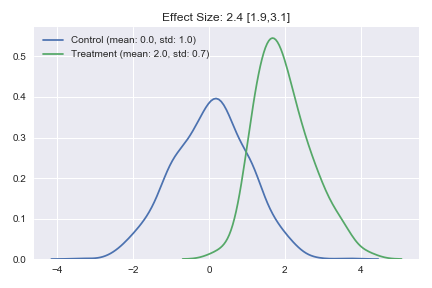
\includegraphics[width=\textwidth]{images/small_es}
%        \caption{The treatment has standard deviation of 0.5, and the effect size is 3.93}
        \label{fig:small_es}
    \end{subfigure}
    \hfill
    \begin{subfigure}[t]{0.49\textwidth}
        \centering
        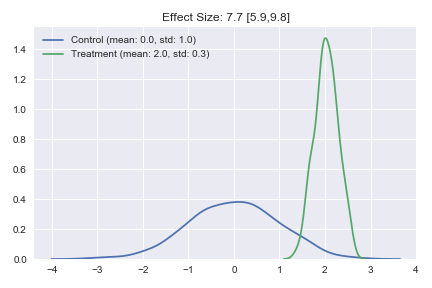
\includegraphics[width=\textwidth]{images/large_es}
%        \caption{The treatment has standard deviation of 0255, and the effect size is 7.77}
		\label{fig:large_es}
    \end{subfigure}
    \caption{Graphical explanation of why the effect size is normalized with the standard deviation of the treatment, when the control has a mean of 0 and standard deviation of 1 and the treatment has a mean of 2; inarguably, the treatment in the right figure the best of the two. Of course, one could perform the same experiment but keeping the treatment fixed and varying the standard deviation of the control: in that case, the effect size would not change. Refer to the main text for a discussion.}
	\label{fig:effect_size}
\end{figure}


Figure \ref{fig:effect_size} shows the effect size computed according to \ref{eq:effect_size}, and tries to provide an intuitive explanation as to why we normalize with the treatment standard deviation. Note that we cannot use an average (weighted or unweighted) as normalizer since it corresponds to assuming homogeneity of \emph{population} variances, an assumption that we wanted to avoid in the first place. Since the goal is to assess the improvement caused by the treatment, it would not make sense to normalize with the standard deviation of the control group, because it would not allow us to discriminate between treatments with the same mean but different standard deviations: given two treatments with the same mean, we prefer the one with the smaller standard deviation. Of course, this reasoning can be applied in the opposite direction: normalizing by the control standard deviation would give a larger effect size when the control group has a smaller standard deviation, which is certainly a desirable property, since a control group with a smaller standard deviation is more clearly separated from the treatment. However, we consider the control group to be fixed, and we will never need to compare two control groups against the same treatment.



\chapter{Method}
\label{ch:method}
This chapter describes how the data is collected (section \ref{sec:data_collection}) and used to re-create the flux-profile relationships (section \ref{sec:profiles}), as well as their prediction based on the Monin-Obukhov similarity theory (section \ref{sec:most_fit}). Then, we describe the main contribution of this thesis, namely how their prediction can be improved using machine learning techniques (section \ref{sec:model_fit}). Finally, we describe how the evaluation is performed (section \ref{sec:perf_eval}), and explicitly state the necessary criteria for a successful answer to the research questions (section  \ref{sec:success}).

\section{Data Collection and Preparation}
\label{sec:data_collection}
The Cabauw Experimental Site for Atmospheric Research\footnote{\url{http://www.cesar-database.nl/}} (Cesar) is a consortium formed by eight Dutch institutes and universities, which collaborate to operate and maintain an observatory for micro-meteorological conditions near the village of Cabauw, the Netherlands. The data collected characterizes the state of the atmosphere and the soil, and their interaction via radiation and surface fluxes.

The observatory is surrounded by fields and no urban agglomerations is present within 15 kilometers; the land is flat with changes of altitude within a few meters over 20 kilometers. The main mast is 213 meters high and offers measurement levels every 20 meters; at each level there are three booms of length 10 meters that allow observations as unobstructed by the main mast as possible, although some disturbance remains. There are three additional smaller masts of height 10 and 20 meters located close to the main mast, in order to obtain undisturbed measurements at the lower levels, and facilities to perform soil and surface observations.

The main focus of this project is on the wind profile and the turbulent fluxes of sensible and latent heat. Additional variables, such as temperature and humidity, are needed to compute quantities of interest, most importantly the Obukhov length, and as possible predictors for the universal functions. There is one measurement for each variable every ten minutes, and missing measurements are gap-filled with a number of techniques. The data collected is always visually validated by an operator, which marks suspect or invalid sections of data.

Following, we describe the instruments used to collect the measurements (section \ref{sec:measurement}), the techniques used to impute missing or invalid measurements (section \ref{sec:gap_filling}), and the criteria applied to filter low quality data (section \ref{sec:data_filter}).

\subsection{Measurement}
\label{sec:measurement}
The Cesar observatory provides full information regarding data collection\footnote{\url{http://projects.knmi.nl/cabauw/insitu/observations/documentation}}, see in particular \cite{cabauwinsitu}, what follows is a brief summary of the sections in that document that are relevant for this work.

\subsubsection{Wind Speed Measurement}
Wind speed and direction are measured at heights of 200, 140, 80, 40, 20 and 10 meters, in either two or all three booms available. The wind vane that measures direction has a resolution of $1.5^\circ$, and the cup anemometer that measures wind speed has an accuracy of the largest between 1\% and \SI{0.1}{\meter\per\second}. \cite{windinstr} studied the threshold sensitivity of both instruments, and fount it lower than \SI{0.5}{\meter\per\second}, even though the measurements are inaccurate up to \SI{3}{\meter\per\second}.

For every ten minutes interval, the measurement comes from the instrument that is best exposed to the wind, and less affected by the obstruction caused by the mast. Corrections are then applied to the raw measurements to further attenuate the disturbance by the tower, following \cite{winddistortion}.

\subsubsection{Eddy Correlation}
\label{sec:eddy_correlation}
The eddy correlation technique is used to compute the turbulent surface fluxes of sensible and latent heat $H$ and $\lambda E$, as well as the momentum flux, starting from fluctuations in wind, temperature, humidity, and $CO_2$ content.

These measurements are obtained with a sonic anemometer and and an optical open-path sensor. Sonic anemometers measure the wind speed by leveraging the fact that the speed of sound in free air is affected by the speed of the air itself; since the speed of sound is known, the wind speed can be easily recovered from the time a sound impulse takes to travel a short distance. By measuring the wind velocity along three orthogonal paths, the full wind vector can be recovered. This measure can then be used to compute the temperature, by leveraging the fact that the speed of sound is affected by the temperature of the medium it travels in. Optical open-path sensors quantify the amount of water vapor and carbon dioxide in the air by emitting a ray of infrared light and measuring its intensity 10 to 20 centimeters further. $H_2O$ and $CO_2$ molecules in the air absorb electromagnetic radiation at known frequencies, thus the concentration of water vapor and carbon dioxide can be inferred by measuring the attenuation at these wavelengths. Some of these instruments are shown in figure \ref{fig:cabauw_180m_instruments}.

All these instruments can take up to 100 measurements per second, necessary in order to compute the turbulence. The eddy correlation technique measures fluxes by computing their sample covariance with the vertical wind speed. Let $w_t$ be the vertical wind speed at time $t$, then the turbulent vertical flux for the quantity $a$ is computed as follows:

$$
F_a=\frac{1}{T_2-T_1}\sum_{t=T_1}^{T_2}(w_t-\overline{w})(a_t-\overline{a})
$$

\noindent where $\overline{w}$ and $\overline{a}$ are the averages of $w_t$ and $a_t$ for $T_1\leq t\leq T_2$. The fluxes in the Cesar database are computed every ten minutes, with 10 measurements per second.

The eddy correlation technique is far from perfect, see e.g. \citep{microhandbook, ed_co2}. Other methods can be used to compute $H$ and $u_*$; for example, \cite{cabauw_abl} uses an iterative method to estimate these quantities from $L$, starting from an initial guess and refining the result, alternating improvements of $u_*$ and $H$ with improvements of $L$.

\subsubsection{Air Temperature and Dew Point Measurement}
Both air temperature and dew point\footnote{the temperature the air needs to be to reach a relative humidity of 100\%} are measured at heights of 200, 140, 80, 40, 20, 10 and 1.5 meters, and the dew point is computed from the air temperature and the humidity obtained with the open-path sensor described previously. The instruments at the highest four levels are located on the main tower, whereas 20 and 10 meters are measured in the smaller mast, and 1.5 meters is measured by the weather station. The resolution of the instruments is of \SI{0.1}{\celsius}, whereas the accuracy is \SI{0.1}{\celsius} for temperature and 3.5\% of relative humidity for the dew point (1.5\% after 2014). Low wind speed and high irradiation can result result in a few \SI{0.1}{\celsius} overestimate of the temperature \citep{tempoverestimate}, whereas the humidity can be over estimated when drying after dew, fog, or rain \citep{cabauwinsitu}.


\begin{figure}
    \centering
    \begin{subfigure}[t]{0.48\textwidth}
        \centering
		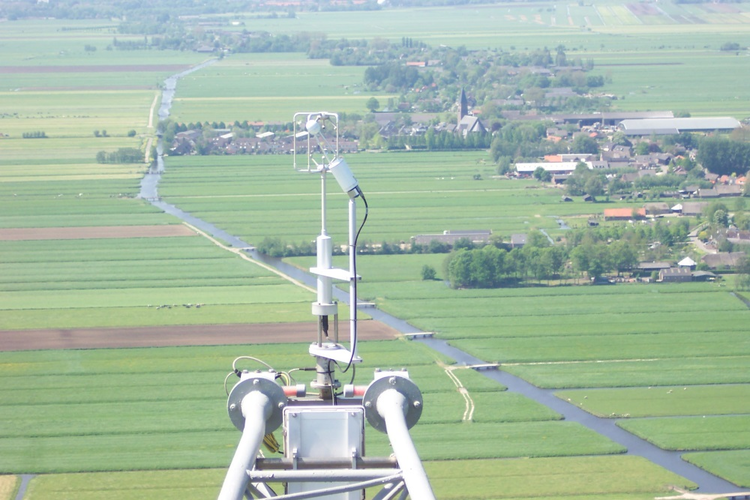
\includegraphics[width=\textwidth]{images/cabauw_turbulence_instruments}
		% https://www.knmi.nl/research/observations-data-technology/projects/cabauw-in-situ-measurements
    \end{subfigure}
    \hfill
    \begin{subfigure}[t]{0.48\textwidth}
        \centering
		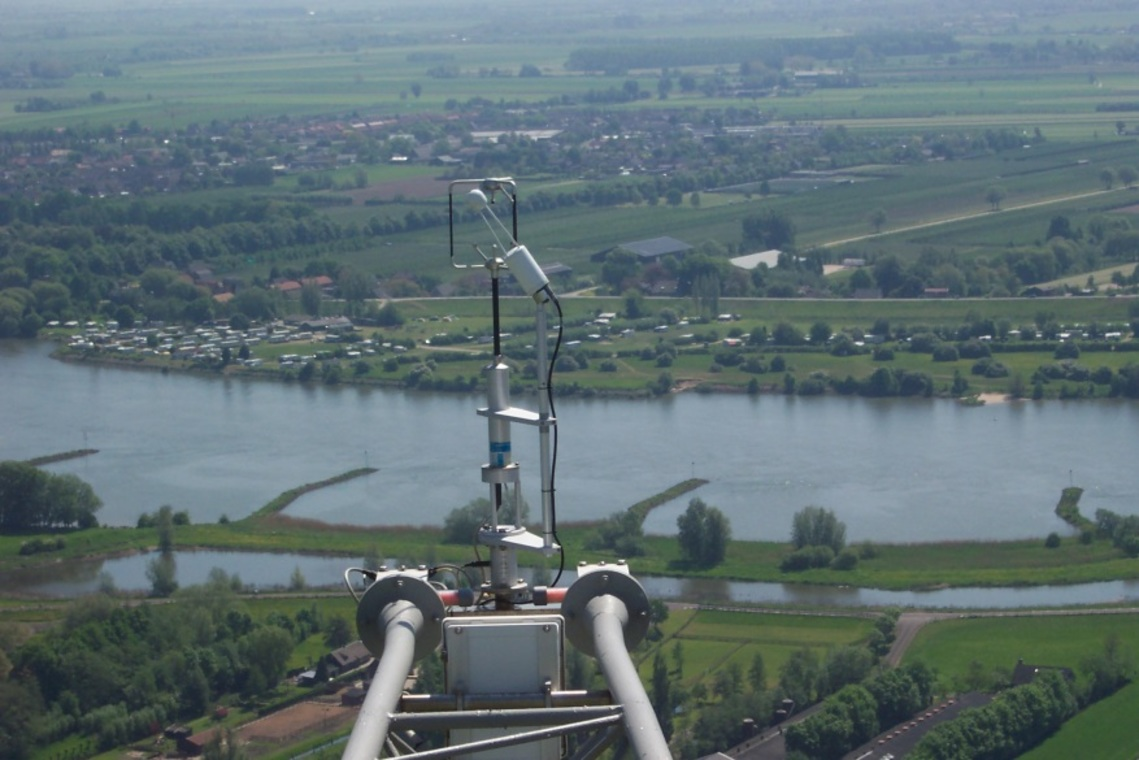
\includegraphics[width=\textwidth]{images/cabauw_turbulence_instruments_2}
		% http://www.knmi.nl/kennis-en-datacentrum/project/cesar-cabauw-and-wind
    \end{subfigure}
\caption{Two of the three sonic anemometers, that measure turbulence, and optical open-path sensor, that measure humidity and $CO_2$, at the 180m level of the Cabauw mast.}
\label{fig:cabauw_180m_instruments}
\end{figure}


\subsubsection{Net Radiation Measurement}
The Cabauw observatory measures both incoming and outgoing long- and short-wave radiation, and the net radiation is simply the combination of these four components. The basic operating principle of an instrument that measures radiation is to have a device coated with paint that is highly absorbing towards a certain range of frequencies; the temperature difference between the surface of this sensor and the body of the whole instrument generates an electrical potential that is proportional to the radiation absorbed by the sensor, after appropriate corrections.  The instruments that measure short-wave radiation are called \emph{pyranometers}, while long-wave radiation is measured by \emph{pyrgeometer}.  The instrument used to measure the net radiation has a pair or pyrgeometers, one facing up and one facing down, to measure the net long-wave radiation, and a pair of pyranometers arranged similarly to measure net short-wave radiation (see figure \ref{fig:net_radiometer}).

This instrument is positioned at \SI{1.5}{\meter} height, and is ventilated and heated to prevent formation of dew, that can make the measurements invalid.


\begin{figure}
    \centering
    \begin{subfigure}[t]{0.4\textwidth}
        \centering
        % https://en.wikipedia.org/wiki/File:Hukseflux_netto_radiometer_nr01_photo.jpg
        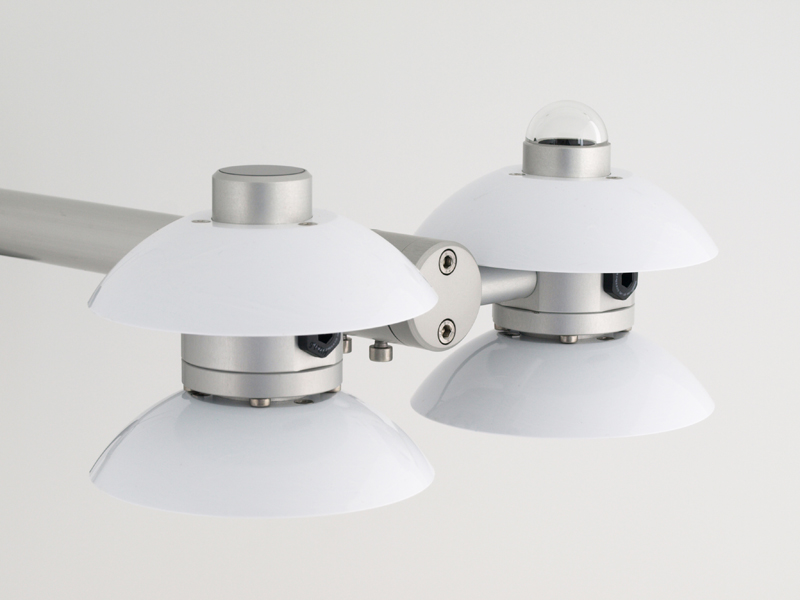
\includegraphics[width=\textwidth]{images/net_radiometer}
        \caption{Net Radiometer}
        \label{fig:net_radiometer}
    \end{subfigure}
    \hfill
    \begin{subfigure}[t]{0.28\textwidth}
        \centering
        % https://en.wikipedia.org/wiki/File:Hukseflux_netto_radiometer_nr01_photo.jpg
        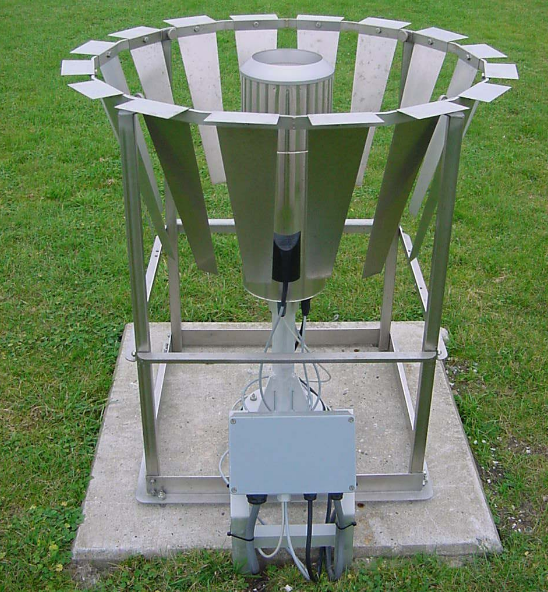
\includegraphics[width=\textwidth]{images/rain_gauge_shield}
        \caption{Rain Gauge with Wind Shield}
        \label{fig:rain_gauge_shield}
    \end{subfigure}
    \hfill
    \begin{subfigure}[t]{0.18\textwidth}
        \centering
        % http://projects.knmi.nl/hawa/pdf/Handbook_H01_H06.pdf
        % aka \citep{rain}
        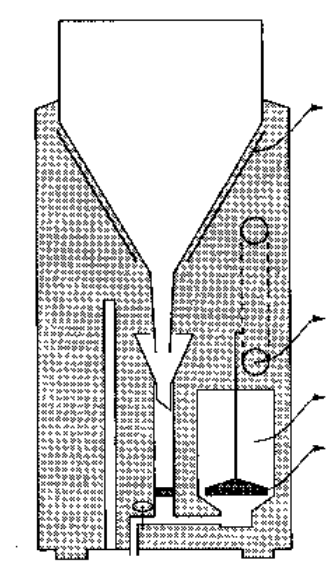
\includegraphics[width=\textwidth]{images/rain_gauge}
        \caption{Rain Gauge Schematic}
        \label{fig:rain_gauge_schematic}
    \end{subfigure}
    \caption[Some instruments used at the Cabauw observatory.]{Some instruments used at the Cabauw observatory. Credits: picture \subref{fig:net_radiometer} - Wikimedia Commons\protect\footnotemark, picture \subref{fig:rain_gauge_shield} - \cite{windsheld_rain}, picture \subref{fig:rain_gauge_schematic} - \cite{rain}.}
	\label{fig:cabauw_instruments}
\end{figure}

% https://tex.stackexchange.com/a/67030
% essentially, cannot have a footnote in a caption or you screw up the lisf of figures at the beginning
% this is latex's simple and intuitive way of saying not to bother about the footnote in the list of figures
\footnotetext{\url{https://en.wikipedia.org/wiki/File:Hukseflux_netto_radiometer_nr01_photo.jpg}}

\subsubsection{Surface Soil Heat Flux}
The surface soil heat flux, measured in \si{\watt\per\square\meter}, is extrapolated from the average fluxes measured at depths of \SI{5}{\centi\meter} and \SI{10}{\centi\meter}; under the assumption of homogeneous soil, the amplitude of the flux in the frequency domain decays exponentially with depth. In order to increase the temporal resolution, the amplitude of the surface soil heat flux is then related to the amplitude of the soil temperature gradient, obtained as the difference between the soil temperature at \SI{0}{\centi\meter} and \SI{2}{\centi\meter}. An inverse Fourier transform converts this surface soil heat flux into the time domain \citep[Appendix~A]{surface_soilheat}. The heat flux is computed by dividing the temperature difference at the top and bottom sides of a plate-shaped sensor\footnote{because of conduction, the temperature of the sensor would tend to homogenize; the higher the difference in temperature, the more energy is hitting the warmer side.} with the horizontal area of the sensor. A \emph{thermocouple} is a device that generates a voltage proportional to this temperature difference, and self-calibrating sensor converts this voltage into a heat flux measurement in \si{\watt\per\square\meter}  \citep{soilheat_sensor}.


\subsubsection{Rain Amount}
The KNMI electronic rain gauge \citep{rain,windsheld_rain} records the average precipitation intensity of the last 12 seconds in \si{\milli\meter\per\second} every 12 seconds, and the rain amount, in \si{\milli\meter}, is derived for every 10 minutes interval. The rain gauge is composed by a heated container in which precipitation accumulates and which is emptied every 12 seconds; the flow of outgoing liquid is measured by a floater connected to a potentiometer, and its value divided by 12 gives the precipitation intensity. The accuracy of the precipitation meter is \SI{0.2}{\milli\meter}, and the precision is \SI{0.1}{\milli\meter}. Figure \ref{fig:rain_gauge_shield} shows the rain gauge with the wind shield \citep{windsheld_rain}, and figure \ref{fig:rain_gauge_schematic} shows a diagram of the instrument \citep{rain}.

\subsection{Gap Filling}
\label{sec:gap_filling}
With gap-filling, missing measurements are replaced by synthetic values \citep{cabauw_gapfilling}. The gap-filling method depends on the missing parameter and the duration of the period where data is not available. There are two classes of parameters: forcing parameters, which include wind, temperature, specific humidity, incoming radiation and rain, and validation parameters, which include the surface fluxes, outgoing radiation, and friction velocity.

For less than two hours of missing measurements, both forcing and evaluation parameters are gap-filled by interpolation of nearby values. For longer periods, forcing parameters are derived by transforming measures obtained from the nearby site of De Bilt, which are themselves gap-filled, if necessary. Evaluation parameters are computed with a vegetation model that uses the forcing parameters as input. The gap-filling procedure is performed by the Cesar consortium, and we do not impute the remaining missing values, since we believe there is a good reason why these values were not gap-filled in the first place.

\subsection{Data Filtering}
\label{sec:data_filter}
Following other works in this field, such as \cite{boulder} and \cite{hogstrom88}, we exclude all the records where any of the following conditions applies:

\begin{itemize}
\item The sensible heat flux $H$ is smaller than \SI{10}{\watt\per\square\meter};
\item The friction velocity $u_*$ is smaller than \SI{0.1}{\meter\per\second};
\item The wind speed $\overline{u}$ is lower than \SI{1}{\meter\per\second}.
\end{itemize}

The reason for this is that the measures are too inaccurate to be of use.


\section{Momentum Flux-Profile Relationship}
\label{sec:profiles}

Since the turbulent fluxes and the friction velocity are measured at the surface level, we can compute the momentum flux-profile relationships only at 10, 20 and 40 meters, because these quantities can be assumed constant only within the surface layer. It is very hard to know the exact height of the surface layer, because it depends on the weather and no exact formulas are known, but it is usually assumed to be 10\% as high as the boundary layer. Based on the typical height of the boundary layer, the surface layer is often higher than 40 meters and lower than 80. \cite{cabauw_z0} indeed reports that a large number of observations from Cabauw at \SI{20}{\meter} are inside the surface layer, the \SI{100}{\meter} level is already outside of the surface layer, and \cite{boulder} used the observations at \SI{50}{\meter} in their analysis, but not those at \SI{100}{\meter}. Moreover, \cite{cabauw60m} reported that the observations at \SI{60}{\meter} are outside of the surface layer only in the early morning; the height of the boundary layer starts growing at around 6 AM, and reaches \SI{600}{\meter} between 9.30 AM and 10.30 AM, and reaches its maximum height, between \SI{1800}{\meter} and \SI{2000}{\meter}, at the end of the day Unfortunately, there is no mention of the \SI{40}{\meter} level in \cite{cabauw60m}. Note that these measures were obtained in May, therefore they are likely to be smaller in Winter, and larger in the Summer. This evidence seems to support the fact that \SI{40}{\meter} is inside the surface layer most of the time.

\subsection{Obukhov Length}

The Obukhov length is computed as in equation \ref{eq:most_l}, reported here:

$$
L=-\frac{u_*^3 T_v}{\kappa g \overline{w'\theta_v}}
$$

The flux of virtual potential temperature can be computed following the formulas in section \ref{sec:most}, as the data contains all the necessary quantities; $u_*$ is given, as well as the specific humidity and the pressure. The Obukhov length is computed at each height level using the corresponding air temperature measurement, and the fluxes measured at the surface.


\subsection{Gradients}
\label{sec:gradients}
The momentum flux-profile relationship is in equation \ref{eq:phi_m}, reported here for the reader's convenience:

$$
\phi_m(\xi)=\frac{\partial\overline{u}}{\partial z}\frac{kz}{u_*}
$$

In order to compute it from the data, we need to compute the derivative of the wind speed with respect to the altitude. In general, the derivative can be obtained by fitting a model on the observations, and computing the derivative using the model. The simplest option is to use a piecewise linear function that passes through the measurements; let the observations be sorted by height and $y_i$ the measurement at height $z_i$, then for $z\in[z_i,z_{i+1}]$ we have:

\begin{equation}
f(z)=y_i+(z-z_i)\frac{y_{i+1}-y_i}{z_{i+1}-z_i}
\end{equation}

The derivative of this function at height $z_i$ is then the average of the slope of the segments that start and end at $z_i$:

\begin{align}
\label{eq:fd_gradient}
\begin{split}
f^\prime(z_i)&=\lim_{h\rightarrow 0}\frac{f(z_i+h)-f(z_i-h)}{2h} \\
&=\frac{1}{2}\cdot\lim_{h\rightarrow 0}\left(\frac{f(z_i+h)}{h}-\frac{f(z_i-h)}{h}\right) \\
&=\frac{1}{2}\cdot\lim_{h\rightarrow 0}\left(
\frac{y_i}{h}+\frac{y_{i+1}-y_i}{z_{i+1}-z_i}-\frac{y_i}{h}+\frac{y_i-y_{i-1}}{z_i-z_{i-1}}
\right)\\
&=\frac{1}{2}\cdot\left(
\frac{y_{i+1}-y_i}{z_{i+1}-z_i}+\frac{y_i-y_{i-1}}{z_i-z_{i-1}}
\right)
\end{split}
\end{align}

In order to compute this derivative at the lowest measured level $z_1=\SI{10}{\meter}$, we can exploit the no-slip condition and introduce an artificial observation $y_0=\SI{0}{\meter\per\second}$ at $z_0$. The value of the \emph{rougness length} $z_0$ depends on the properties of the surface, and, although no unambiguous value is known for the Cabauw observatory, its value is likely between $10^{-1}$m and $10^{-2}$m \citep{cabauw_z0, cabauw_night}, therefore it is reasonable to conclude that its effect is negligible on the final gradient.

A more complicated model, introduced by \cite{windlogprofile}, is

\begin{equation}
\label{eq:logmodel}
f(z)=a+bz+cz^2+d\ln z
\end{equation}

The model is linear in its parameters, therefore equation \ref{eq:ridge_solution} can be used to compute the coefficients, using the feature mapping $\phi(z)=\left[1,z,z^2,\ln z\right]^\intercal$ and regularization parameter $\lambda=0$. Once the coefficients are known, the gradient is trivial to compute:

\begin{equation}
\label{eq:log_gradient}
f^\prime(z)=b+2cz^2+d\frac{1}{z}
\end{equation}

After removing the observations for which this model has a $R^2<0.9$, \cite{windlogprofile} estimates the uncertainty of this gradient to be around 30\%. Note that some works, such as \cite{windprof_nosqr}, do not use the squared term.

Finally, a third method of computing the gradient is to fit a Gaussian process to the profile using the following kernel:

\begin{equation}
\label{eq:kernel}
k(z_1,z_2)=\exp\left(-\frac{(z_1-z_2)^2}{2\sigma_0^2}\right)+\sqrt{\sigma_1^2+ z_1 z_2}+\sigma_2^2 \mathbbm{1}[z_1=z_2]+\sigma_3^2
\end{equation}

\noindent where $\mathbbm{1}[P]$ is an indicator function whose value is 1 if the predicate $P$ is true, and 0 otherwise, and the parameter $\sigma_2$ controls the noise in the measurement. Unfortunately, this noise is not constant, and does not depend on the altitude level; for example, for the wind speed $u$, the precision of the instrument is $\max(0.1,0.01\cdot u)$. Therefore, all the parameters must be found by optimizing the marginal likelihood. Figure \ref{fig:kernel} shows the prior distribution of a Gaussian process with this kernel, as well as the value of the kernel for some choices of $z_1$ and $z_2$.

\begin{figure}
    \centering
    \begin{subfigure}[t]{0.45\textwidth}
        \centering
        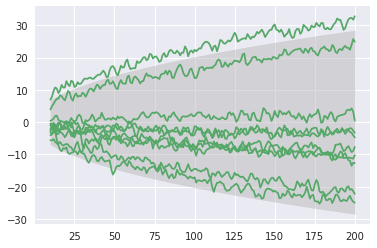
\includegraphics[width=\textwidth]{images/profile_kernel_prior}
        \caption{Prior distribution and some samples; the grey area is the 95\% CI.}
        \label{fig:kernel_prior}
    \end{subfigure}
    \hfill
    \begin{subfigure}[t]{0.45\textwidth}
        \centering
        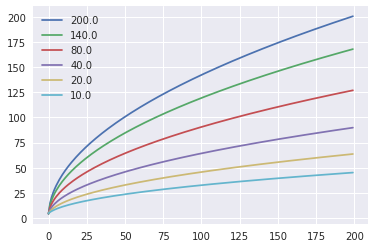
\includegraphics[width=\textwidth]{images/kernel_values}
        \caption{Values of the kernel: each line corresponds to a different value of $z_1$, and $z_2$ is on the ordinate.}
        \label{fig:kernel_values}
    \end{subfigure}
    \caption{Behavior of the kernel in equation \ref{eq:kernel}, where the altitude is on the $x$ axis, and the predicted value on the $y$ axis. Notice the approximate logarithmic profile with which the predicted value changes with altitude; this is caused by the square root term in the kernel, and emulates the effect of the $\ln z$ term in equation \ref{eq:logmodel}.}
	\label{fig:kernel}
\end{figure}

Our final goal is to obtain the derivative of the predictive posterior mean, which can be done using equation \ref{eq:gp_gradient}; for this we need to derive equation \ref{eq:kernel} with respect to $z_1$:

\begin{equation}
\label{eq:kernel_derivative}
\frac{\partial k(z_1,z_2)}{\partial z_1}=\frac{z_2-z_1}{\sigma_0^2}\exp\left(-\frac{(z_1-z_2)^2}{2\sigma_0^2}\right)+\frac{z_2}{2\sqrt{\sigma_1^2+z_1z_2}}+\sigma_2^2\mathbbm{1}[z_1=z_2]
\end{equation}



\section{Monin-Obukhov Similarity Theory}
\label{sec:most_fit}

Even though there is agreement on form of the momentum flux-profile relationship, there is still debate on the exact values of the coefficients, with different experiments resulting in different values \citep{hogstrom88}. In order to ensure a fair comparison with the results of this work, we fit the universal functions to the data from the Cesar database. Their general form is:

\begin{equation}
\label{eq:phi_general}
\phi(\xi)=\begin{cases}
a+b\xi & \xi\geq 0 \\
a(1-c^2\xi)^d & \xi<0 \\
\end{cases}
\end{equation}

Where $a$ is close to 1, $b$ is positive, and $d$ is negative. Since $d$ is negative, the base of the power must be positive, hence the squared $c$. Following the approach outlined in section \ref{sec:regression_fit}, the coefficients $a$, $b$, $c$ and $d$ can be found by minimizing the L2-regularized mean squared error using equations \ref{eq:least_squares_gradient} and \ref{eq:least_squares_hessian}; in this case, the parameter vector is $\bm\theta=\left[a,b,c,d\right]^\intercal$. The gradient of \ref{eq:phi_general} is:


\begin{align}
\nabla_\theta\phi(\xi)\vert_{\xi\geq 0}=\begin{bmatrix}
1 \\ \xi \\ 0 \\ 0
\end{bmatrix} &&
\nabla_\theta\phi(\xi)\vert_{\xi<0}=\begin{bmatrix}
\tau^d \\ 0 \\ -2acd\xi\tau^{d-1} \\ a\tau^d\ln\tau
\end{bmatrix}
\end{align}

\noindent where $\tau=1-c^2\xi$. The Hessian of \ref{eq:phi_general} when $\xi\geq 0$ is simply 0, because it is a linear function in all parameters, while, in the negative case, we have:

\begin{equation}
\nabla^2_\theta\phi(\xi)\vert_{\xi<0} = \begin{bmatrix}
0 & 0 & - 2 c d \xi \tau^{d - 1} & \tau^{d} \ln{\tau} \\
0 & 0 & 0 & 0 \\
- 2 c d \xi \tau^{d - 1} &
0 & \frac{2ad\xi\tau^{d}}{c^4\xi^2+\tau}\left(2c^2d\xi-c^2\xi-1\right) & -2ac\xi\tau^{d-1}\left(d\ln\tau+1\right) \\
\tau^d \ln\tau & 0 &
-2ac\xi\tau^{d-1}\left(d\ln\tau+1\right) &
\tau^d\ln^2\tau
\end{bmatrix}
\end{equation}

Analytical computation of the Hessian allows us to use the Newton conjugate gradient descent algorithm, which provides super-linear convergence rate, unlike other conjugate gradient methods whose rate of convergence is only linear \citep{numopt}. This model is then fitted to the data using L2 regularization, and evaluated as the other regression models.

\section{Model Fitting}
\label{sec:model_fit}
In this section, we discuss how we use the data from the Cesar database to predict $\phi_m$.

\subsection{Features}
All the features come from the Cesar database. The predictors are partitioned in five sets:

\begin{enumerate}
\item[F1:] soil temperature, altitude $z$, wind at $z$, temperature at $z$, wind at 10 meters, temperature at 10 meters, wind at 20 meters, temperature at 20 meters, wind at 40 meters, temperature at 40 meters;
\item[F2:] Soil heat flux;
\item[F3:] Net radiation;
\item[F4:] Rain amount, dew point;
\item[F5:] Turbulent kinetic heat flux $H$, turbulent latent heat flux $\lambda E$;
\end{enumerate}

These sets are used cumulatively in the order they are listed, meaning that F2 is used in conjunction with F1, F3 with F2 and F1, and so on. Features that can be computed from others, such as the virtual temperature (equation \ref{eq:vtemp}), are not included. The reason is that the less inputs the models require, the more useful and "agile" they can be when used as a component in a larger system, such as climate simulations: reducing the amount of computations makes the simulation faster and reduces numerical errors, since many approximate constants have to be used. Moreover, one of the objectives of this work is to quantify the effect of the feature sets on the prediction accuracy; using derived features would actually make this process difficult, since the point of it is to find the fundamental quantities of importance.

This division was decided based on the knowledge of a domain expert, so that the level of a feature reflects both its expected impact on the performance and how desirable it is to include it. An example of the former reasoning is with F4, where the effect of moisture is expected to be already captured by the soil heat flux (in F2), and to be generally negligible in all but the most extreme conditions. An example of the latter reasoning is with F5, because turbulent fluxes are hard to measure accurately (see section \ref{sec:eddy_correlation}), and current simulation models are known to be quite inaccurate in their estimation of these fluxes \citep{sheba}. Similarly, the friction velocity was not included, because the point of predicting $\phi_m$ is to use it to estimate $u_*$ from the wind gradient, which is readily measured both in real life and in simulations. \cite{cabauw_z0} has shown that the direction of the wind affects the universal functions at Cabauw, because of the different covers of the surface, changing the roughness length, and disturbances by the main mast, preventing accurate wind speed measurement. Nonetheless, we decided not to include the wind direction in the features, as this is very specific to the Cabauw observatory, and would reduce the generality of our models.

We also create a second version of each feature set, augmented with the hourly trend of each variable, except for the altitude $z$. The reason for including the trend is that it can give an indication of, for example, the time of the day, or other complex phenomena for which there is no measurement. The interval for the trend (one hour) is used because it is enough to capture local variations, but not too large so as to contain irrelevant information. The hourly trend is computed simply as the difference between the current value and the value measured one hour before, divided by one hour. Given the goal of this work, namely to produce a model to be used in climate simulations, it would not make sense to use future values to compute the trend.

Finally, each feature is centered and standardized so as to have zero mean and unit standard deviation:

\begin{equation}
\label{eq:standardization}
x^\prime_{i,j}=\frac{x_{i,j}-\mu_j}{\sigma_j}
\end{equation}

This method is not robust to outliers, since they heavily affect mean and standard deviation; this can be prevented by subtracting the median and normalizing with the interquartile range instead. These two methods give similar results in our datasets, therefore we follow equation \ref{eq:standardization}, since it it the most widely used in practice. Obviously, every $\mu_j$ and $\sigma_j$ are computed only on the training data, and used to normalize both training and testing data.

\subsection{Estimators}

The models that we use are ridge regression, k-nearest neighbors, gradient boosted trees, and neural networks. Due to the size of the dataset, we cannot use kernel-based algorithms such as SVM and Gaussian Processes, as they require $\Theta(N^2)$ memory to store the kernel matrix, and $O(N^3)$ time to invert it.

All models but neural networks are fitted using nested cross validation with random hyper-parameter search. This procedure detailed in section \ref{sec:perf_eval}, but we list here the distributions of the hyper-parameters that we use in the random search:

\begin{itemize}
\item Ridge regression and Monin-Obukhov estimator: the only hyper-parameter to tune is the regularization coefficient, for which we use a log$_{10}$-uniform distribution\footnote{a random variable $X$ has a log$_\beta$-uniform distribution from $a$ to $b$ if $\log_\beta X$ is uniformly distributed between $a$ and $b$. Equivalently, if $Y$ is uniform between $a$ and $b$, then $\beta^Y$ is log$_\beta$-uniform.} from $10^{-6}$ to $10^{1}$.

\item k-nearest neighbors: the hyper-parameters to tune are the number of neighbors, chosen uniformly from $1$ to $15$, the distance function, either L1 or L2 norm, and the weights of the neighbors, either uniform or directly proportional to the distance to the query point.

\item Gradient boosted trees: the distributions are shown in table \ref{tbl:gb_hyperparams}. Note that $\delta$, for the Huber loss, refers to the percentile of the residuals, so that $\delta=0.5$ uses L2 loss for the smallest 50\% and L1 loss for the largest 50\%.
\end{itemize}

We use log-uniform distributions for parameters with a high range of possible values to reflect the intuition that small values are as likely as large values, and to avoid the samples being dominated by the larger values. Samples from an uniform distribution from $10^0$ to $10^3$ are ten times more likely to be from $[10^2,10^3]$ than from $[10^1,10^2]$, and, on average, only one in 100 samples will be in $[10^0,10^1]$. Log$_{10}$-uniform distributions do not have this problem, and a sample is equally likely to belong to any of the three intervals.

\begin{table}[]
\centering
\caption{Distribution of the hyper-parameters for gradient boosted trees}
\label{tbl:gb_hyperparams}
\begin{tabularx}{\textwidth}{r|l|X}
\toprule
\textbf{Hyper-parameter} & \textbf{Distribution} & \textbf{Values} \\ \midrule
Number of estimators & Log$_{10}$-uniform & From $10^1$ to $10^4$ \\
Learning rate & Log$_{10}$-uniform & From $10^{-3}$ to $10^0$ \\
Number of features & Uniform & All possible values \\
Maximum depth & Uniform & From 4 to 12 \\
Sub-sampling factor & Uniform & From 25\% to 100\% \\
Loss function & Uniform & Least squares, least absolute deviation, \newline Huber loss (equation \ref{eq:huberloss}) \\
$\delta$ (for the Huber loss) & Uniform & From 1\% to 99\% \\
\bottomrule
\end{tabularx}
\end{table}



\section{Performance Evaluation}
\label{sec:perf_eval}
The goal of performance evaluation is to obtain a realistic and unbiased estimate of the performance of a model on unseen data. Because the Monin-Obukhov similarity theory is only valid in the $-2\leq\xi\leq1$ range, we will use this data as the primary target for evaluation. We will also evaluate the models on the full dataset, to see what kind of performance can be expected outside of the typical range where the similarity theory is employed.

\subsection{Evaluation Procedure}
The two research questions require different evaluation procedures. The first question essentially entails finding what kind of performance is possible to achieve: this is best done using nested cross-validation, so that this estimate is not biased. The second research question is about comparing alternatives: in this case, we use repeated cross-validation to obtain estimates with lower variance. In both cases we use random search \citep{random_search} to optimize the hyper-parameters of the models.

For nested cross-validation, we use 10 outer folds and 10 inner folds, and try 10 random hyper-parameter combinations. Since we have 2 datasets and $5\cdot2$ feature sets, every model is fit a total of $2\cdot5\cdot2\cdot(10\cdot10\cdot10+10)=20200$ times. For repeated cross-validation, we use 10 folds and 25 hyper-parameters combinations, resulting in 250 fittings.

todo how many repeats? better be fixed!

According to the model and its hyper-parameters, fitting can take from a few seconds up to more than 24 hours; in order to make the process feasible, we implemented algorithm \ref{alg:nested_cv} using Apache Spark \citep{spark}. Since the number of stragglers is very low\footnote{for gradient boosted trees, the slowest method, the median fitting time in our experiments is around half a minute, the third quartile is around ten minutes, and the maximum is between 20 and 30 hours}, running multiple nested cross validation jobs at the same time can reduce the duration of the whole process by five to ten times.

A fundamental assumption underlying hold-out evaluation methods is that the samples in the training set are independent and identically distributed, so that the distribution in the two partitions are equal. This is not our case, since there is a inherent time dependency in the data, meaning that samples obtained close in time are very similar. This can be confirmed by training and evaluating a k-nearest neighbors classifier with $k=1$ on random splits: the resulting mean squared error is in the order of $10^{-3}$, which is clearly unrealistic. To circumvent this problem, the CV folds are created on \emph{months}: all the samples in a given month and year are either in the training set or in the validation set. We choose months instead of days because the weather often does not change significantly in the span of 24 hours, whereas in a month there are around three weeks worth of samples that are independent from the conditions at the start and end of the month.

\subsection{Evaluation Metrics}
The main evaluation metric is the mean squared error, since that is what we are optimizing for, but we compute other metrics in the outer cross validation loop to get a more complete idea of the performance of the estimators:

\begin{itemize}
\item Mean Squared Error (MSE);
\item Mean Absolute Error (MAE);
\item Median Absolute Error (mAE);
\item Mean Absolute Percent Error (MAPE);
\item Median Absolute Percent Error (mAPE);
\item $R^2$ Score:
$$
1-\frac{\sum (f_n-t_n)^2}{\sum (t_n-\overline{t})^2}
$$
\end{itemize}

Where $f_n$ is the predicted value for the test sample $\bm x_n$ with true value $t_n$, the squared error is $(f_n-t_n)^2$, the absolute error is $\vert f_n-t_n\vert$, the absolute percent error is $100\vert 1-f_n/t_n\vert$. We present both mean and median scores because the former are heavily skewed by outliers. We also present both absolute and percent errors because the latter are easier to interpret, but tend to explode when the true value is very small,\footnote{predicting 1 for a true value of 100 gives a percent error of 99\%, but predicting 100 for a true value of 1 gives, somewhat unfairly, a percent error of 9900\%, whereas their absolute error is identical.} a condition that frequently happens in our dataset.


\section{Success Criteria}
\label{sec:success}
A successful answer to the first research question entails finding a model whose mean squared error on any feature set, with or without trend, is smaller than the mean squared error of the MOST estimator introduced in section \ref{sec:most_fit}. The second research question is answered by comparing the mean squared error obtained on the ten feature sets (F1 to F5, with and without trend). This comparison is done using the model that achieved the best performance when answering the first research question.

Note that we cannot use the output of a model to obtain the importance of the features, as this method is not reliable when some of them are correlated \citep{rf_bias,rf_corr_imp}, which is a very relevant issue in our case. Trivially, wind speed and temperature at the different levels are very strongly correlated (Pearson's $r$ is above 0.95), and there are other, more complex, correlations, such as between the net radiation and the soil heat flux, or between the soil temperature and the dew point (Pearson's $r$ is respectively 0.75 and 0.79). In spite of the correlations, all these variables contribute to the flux-profile relationships, often in very nuanced ways.

The differences are quantified using the effect size as described in section \ref{sec:effect_size}. We prefer the effect size over the mean MSE because the effect size allows us to consider the standard deviation of the MSE, as well as its mean; this could lead us to prefer models with slightly worse average MSE, but more consistent and reliable performances (i.e. smaller standard deviation). Since we are looking for an improvement, we compute the right 95\% confidence interval for the population effect size. In other words, besides providing a point estimate for the population effect size $\delta_{pop}$, we also provide an interval $[\delta_{low}, \infty)$ that contains it 95\% of the times. We say the treatment is better if $\delta_{low}>0$.

\chapter{Results}
\label{ch:results}

This chapter presents the results obtained following the procedures outlined in chapter \ref{ch:method}. Section \ref{sec:eda} describes the dataset and shows some of its peculiarities, then section \ref{sec:res_gradient} identifies the best method to compute the gradient of the profile, finally section \ref{sec:most_res} shows the momentum flux-profile relationship obtained on the dataset and its predictions from the estimators we discussed previously.

All the processing was done using the Python programming language\footnote{\url{https://www.python.org/}} and the usual Data Science library stack, in no particular order: Pandas \citep{pandas}, scikit-learn \citep{sklearn}, SymPy \citep{sympy}, Matplotlib \citep{matplotlib}, Seaborn\footnote{\url{https://doi.org/10.5281/zenodo.883859}}, NumPy \citep{numpy}, Jupyter Notebook \citep{jupyter}, IPython \citep{ipython}, Spark \citep{spark}, with the crucial support of Hopsworks \citep{hops}


\section{Exploratory Data Analysis}
\label{sec:eda}
The dataset consists of 17 years of measurements, from January 2001 to December 2017, for a total of 3,436,416 observations. The Cesar database contains one tar-gzipped archive for every month, whose content is a single data file in the netCDF format \citep{netcdf}. The archives contain a subset of related variables, and we used the datasets containing surface fluxes, tower meteorological profiles, meteorological surface  data, and soil heat, for a total of 816 datasets covering 204 months.

Unfortunately, most of these observations contain unreliable measurements, as detailed in section \ref{sec:data_filter}, leaving only  1,561,973 usable records. Additionally, the turbulent fluxes measured in March 2016 exhibit a much wider range than the March measurements of other years. Roughly 15 to 20\% of the measurements in that month are suspicious; since the Cesar database contains a separate dataset every month, we decided to completely exclude the dataset of March 2016, fearing for a systematic error somewhere in the process. Moreover, 6 measurements of the turbulent latent heat are way above the acceptable range, 4,538 do not have a dew point, and 247,656 do not have a soil temperature; this leaves 1,308,362 usable records. Table \ref{tbl:col_summary} summarizes the weather parameters that were used to compute the similarity functions and/or as features for the models, and table \ref{tbl:col_gapfilled} presents the number of observations that were gap-filled with each method, for the measurements for which this information was provided.

\begin{table}[]
\centering
\caption{Basic descriptive statistics of the features in the Cesar database, except for the air density and virtual air temperature, which were computed by us.  Note that the relative humidity was computed by the Cesar consortium using values from other measurements, and 16,833 records  (1.3\%) have a relative humidity above 100\%.}
\label{tbl:col_summary}
\begin{tabular*}{\textwidth}{l| @{\extracolsep{\fill}} rrrrrrr}
\toprule
& \textbf{Mean} & \textbf{Std.} & \textbf{Min.} & \textbf{25\%} & \textbf{50\%} & \textbf{75\%} & \textbf{Max.} \\ \midrule
\textbf{$H$} & 3.7 & 47.3 & -460.0 & -25.8 & -14.7 & 28.2 & 479.6 \\
\textbf{$\lambda E$} & 74.7 & 114.9 & -534.8 & -4.9 & 23.8 & 132.9 & 6,940.8 \\
\textbf{$u_*$} & 0.3 & 0.1 & 0.1 & 0.2 & 0.3 & 0.4 & 1.8 \\
\textbf{Wind Speed} & 5.9 & 2.6 & 1.0 & 4.0 & 5.4 & 7.2 & 29.4 \\
\textbf{Air Temp.} & 284.7 & 6.4 & 259.6 & 280.1 & 284.8 & 289.4 & 306.9 \\
\textbf{Soil Temp.} & 284.4 & 5.7 & 271.9 & 279.6 & 284.3 & 289.1 & 302.6 \\
\textbf{Dew Point} & 280.3 & 6.1 & 188.0 & 276.6 & 280.6 & 284.7 & 296.7 \\
\textbf{Spec. Hum.} & 6.6 & 2.5 & -0.9 & 4.8 & 6.4 & 8.3 & 17.8 \\
\textbf{Rel. Hum.} & 76.5 & 15.2 & 0.0 & 66.9 & 79.2 & 88.3 & 133.7 \\
\textbf{Air Press.} & 1,009.6 & 69.0 & 960.9 & 1,008.3 & 1,014.8 & 1,020.7 & 1,046.4 \\
\textbf{Rain Amount} & 0.0 & 0.1 & 0.0 & 0.0 & 0.0 & 0.0 & 15.1 \\
\textbf{$CO_2$ Flux} & -0.1 & 0.3 & -7.5 & -0.2 & 0.0 & 0.1 & 6.1 \\
\textbf{Soil Heat Flux} & 2.9 & 15.6 & -77.8 & -6.5 & -0.7 & 8.9 & 1,139.0 \\
\textbf{Net Rad.} & 81.8 & 167.2 & -158.5 & -35.4 & -3.0 & 172.5 & 7,775.4 \\
\textbf{Air Dens.} & 0.3 & 0.1 & 0.1 & 0.2 & 0.3 & 0.3 & 2.8 \\
\textbf{Virt. Air Temp.} & 1,443.8 & 454.9 & 124.8 & 1,104.2 & 1,391.0 & 1,753.2 & 3,506.0 \\
\bottomrule
\end{tabular*}
\end{table}


\begin{table}[]
\centering
\caption{Number of measurements by gap filling method, for the quantities that have this information. Due to inconsistencies in the Cabauw Documentation \citep{cabauw_gapfilling}, we cannot be sure of the meaning of the columns, but this is our interpretation: 0 - Unknown, 2 - Cabauw In situ (i.e. from the masts, not gapfilled), 3 - Automatic Weather Station in Cabauw (also not gapfilled, but sometimes secondary source), 4 - Computed from profiles, 5 - Interpolated, 6 - Cabauw-based model, 7 - De Bilt-based model. As the net radiation cannot be obtained from the profiles, we think that sources 4 and 5 for this quantity are mistakes, and should respectively be 6 and 7.}
\label{tbl:col_gapfilled}
\begin{tabular*}{\textwidth}{l| @{\extracolsep{\fill}} rrrrrrr}
\toprule
& \textbf{0} & \textbf{2} & \textbf{3} & \textbf{4} & \textbf{5}  & \textbf{6}  & \textbf{7} \\ \midrule
\textbf{$H$} & - &  1,192,346 & - & - &  17,291 &  97,720 &  1,005 \\
\textbf{$\lambda E$} & - &  1,180,434 & - & - &  18,503 &  97,846 &  11,579 \\
\textbf{$u_*$} & - &  1,174,593 & - &  132,461 &  465 &  618 &  225 \\
\textbf{Wind Speed} & - &  1,302,308 &  2,338 & - &  879 &  331 &  2,506 \\
\textbf{Air Temp.} & - &  1,298,075 & - & - &  2,419 &  5,959 &  1,909 \\
\textbf{Spec. Hum.} & - &  1,292,626 & - & - &  3,149 &  10,693 &  1,894 \\
\textbf{Air Press.} &  7,096 & - &  1,298,205 & - &  654 & - &  2,407 \\
\textbf{Rain Amount} &  7,096 &  1,181,167 &  117,844 & - &  346 & - &  1,909 \\
\textbf{$CO_2$ Flux} & - &  964,749 & - & - &  48,983 &  287,855 &  6,775 \\
\textbf{Soil Heat Flux} & - &  1,232,822 & - & - & - &  72,256 &  3,284 \\
\textbf{Net Radiation} & - &  1,274,106 & -&  20,962 &  1,715 & - &  11,579 \\
\bottomrule
\end{tabular*}
\end{table}



Figure \ref{fig:le_season} shows the turbulent latent heat flux versus hour of day both in Winter and Summer, whereas figure \ref{fig:ustar_wind_temp} shows the friction velocity as a function of air temperature and wind speed. The dependency of $u_*$ with the wind speed of figure \ref{fig:ustar_wind} is quite complicated: there are three clear regions with different constant of proportionality and correlation coefficient. The group where the two quantities are almost perfectly correlated corresponds to imputed values for the friction velocity, derived from the wind speed. The three other groups differ widely in the values of the fluxes and radiation; for example, fitting an ordinary least squares model to 1000 bootstraps of the observations with negative net radiation yields an average proportionality coefficient of \num{0.051} with standard deviation \num{1.52e-05}, whereas the same procedure on the complementary set yields an average of \num{0.046} with standard deviation \num{1.40e-05}. Note that this dependency might be related to the observed imbalance in the surface energy budged, usually around 15\% during day time and 100\% during night time at the Cabauw observatory; \cite{cabauwinsitu} notes that the imbalance seems to depend on the speed of wind.

\begin{figure}
    \centering
    \begin{subfigure}[t]{0.48\textwidth}
        \centering
        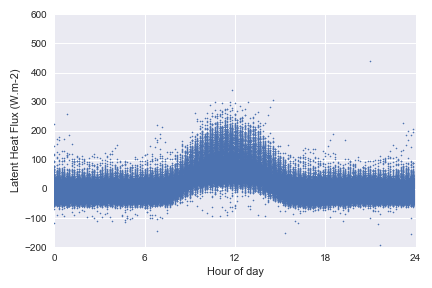
\includegraphics[width=\textwidth]{images/le_winter}
        \caption{Winter}
        \label{fig:le_winter}
    \end{subfigure}
    \hfill
    \begin{subfigure}[t]{0.48\textwidth}
        \centering
        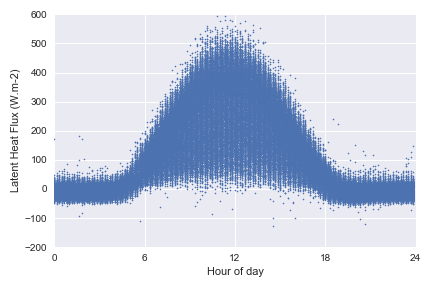
\includegraphics[width=\textwidth]{images/le_summer}
        \caption{Summer}
        \label{fig:le_summer}
    \end{subfigure}
    \caption{Turbulent latent heat flux versus hour of day in Winter (left) and Summer (right). One can see both the difference in day duration, and the effect of increased temperature on evaporation and transpiration. The sensible heat flux follows a very similar pattern, with lower absolute values.}
	\label{fig:le_season}
\end{figure}


\begin{figure}
    \centering
    \begin{subfigure}[t]{0.48\textwidth}
        \centering
        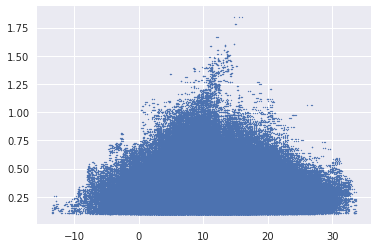
\includegraphics[width=\textwidth]{images/ustar_temp}
        \caption{Temperature}
        \label{fig:ustar_temp}
    \end{subfigure}
    \hfill
    \begin{subfigure}[t]{0.48\textwidth}
        \centering
        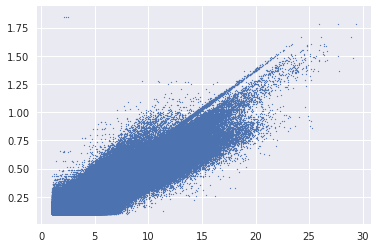
\includegraphics[width=\textwidth]{images/ustar_wind}
        \caption{Wind}
        \label{fig:ustar_wind}
    \end{subfigure}
    \caption{Friction velocity versus temperature (left) and wind speed (right). There is a clear subgroup where the wind and $u^*$ are almost perfectly correlated; this is because of the gap-filling technique discussed in section \ref{sec:gap_filling}. Additionally, there are three subgroups with different regression line fit; they differ widely in fluxes, radiation, and altitude (since $u_*$ is computed at the surface, the intercept is different, because wind speed tends to be positively correlated with altitude).}
	\label{fig:ustar_wind_temp}
\end{figure}



Figure \ref{fig:tsne} shows the result of the t-SNE dimensionality reduction algorithm \citep{tsne} applied to 250,000 samples (19.2\% of the total), using the same features of table \ref{tbl:col_summary}, plus $z$, $L$, $\xi$, the wind and virtual temperature gradients, $\phi_m$, the month of the year and hour of day. The 250,000 samples were chosen uniformly at random and standardized with equation \ref{eq:standardization} before fitting, but the colors were computed using the raw features on a perceptually uniform color scale, after excluding the top and bottom 1\% values. Overall, the points cluster in a relatively uniform blob, which is not surprising once you consider that the measurements were taken continuously, meaning that all physical quantities change smoothly, thus all points close in time are also close in feature space.

The colors reveal some structure, though: the left-hand side of the blob contain measurements taken in the Summer, and the right-hand side contains measurement in Winter (see the air temperature in figure \ref{fig:tsne_temp} and month in figure \ref{fig:tsne_month}). Moreover, unstable conditions are clustered in a stripe, centered vertically, that runs from left to right (see the fluxes of figures \cref{fig:tsne_H,fig:tsne_LE,fig:tsne_soilheat}, the radiation in figure \ref{fig:tsne_netrad}, and the hour of day in figure \ref{fig:tsne_hday}). In figure \ref{fig:tsne_z} we also a see cluster on the top with all the observations at 40 meters, whereas the two lower levels are mixed somewhat uniformly in the bottom part of the plot.

Finally, figure \ref{fig:tsne_clus} shows the result of k-means clustering in the standardized feature space, using $k=2$ (blue/orange) and $k=4$ (the four shades). This clustering is consistent with the qualitative division above, with the dark orange and blue clusters corresponding to Summer and Winter respectively, light orange corresponding to unstable conditions with considerable vertical movement of air, and light blue corresponding to strong horizontal winds with little movement in the vertical. Stably stratified conditions seem to occur at the boundary of the blob, where $\phi_m$ takes the highest values (see figure \ref{fig:tsne_phi_m}). This is also not surprising, since stable stratification tend to happen at night throughout the year, unlike free convection or z-less scaling, which only happen in specific conditions.

\begin{figure}
\subcaptionbox{Air Dens.\label{fig:tsne_air_dens}}{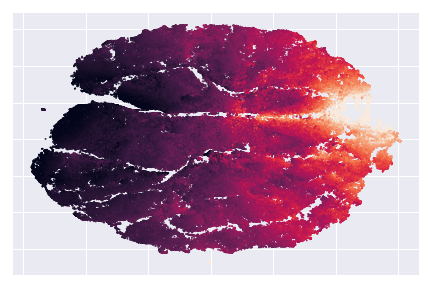
\includegraphics[width=0.25\textwidth]{images/tsne_air_dens}}\hfill
\subcaptionbox{H\label{fig:tsne_H}}{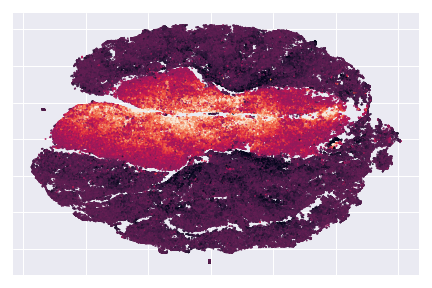
\includegraphics[width=0.25\textwidth]{images/tsne_H}}\hfill
\subcaptionbox{LE\label{fig:tsne_LE}}{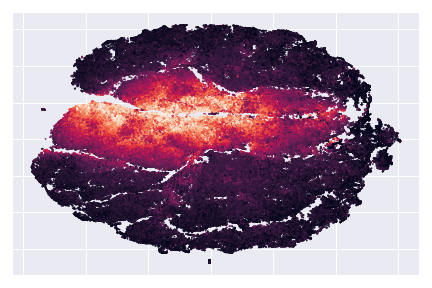
\includegraphics[width=0.25\textwidth]{images/tsne_LE}}\hfill
\subcaptionbox{Wind Speed\label{fig:tsne_wind}}{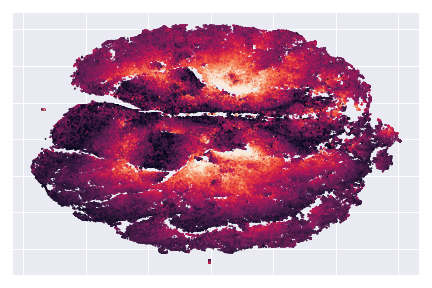
\includegraphics[width=0.25\textwidth]{images/tsne_wind}}\\

\subcaptionbox{Air Temp.\label{fig:tsne_temp}}{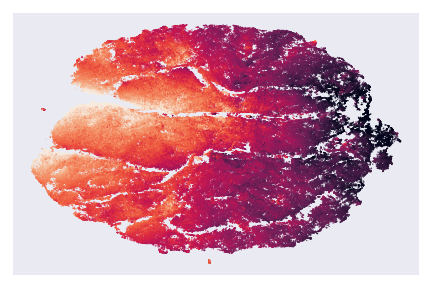
\includegraphics[width=0.25\textwidth]{images/tsne_temp}}\hfill
\subcaptionbox{Virtual Temp.\label{fig:tsne_virtual_temp}}{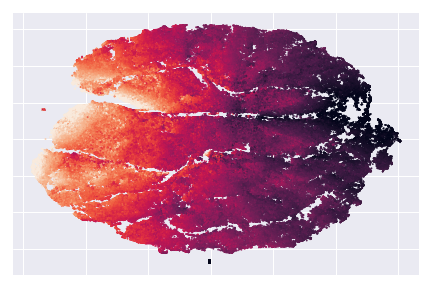
\includegraphics[width=0.25\textwidth]{images/tsne_virtual_temp}}\hfill
\subcaptionbox{Soil Temp.\label{fig:tsne_soil_temp}}{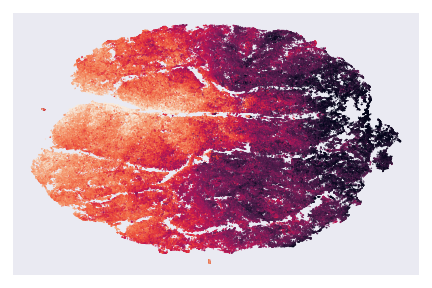
\includegraphics[width=0.25\textwidth]{images/tsne_soil_temp}}\hfill
\subcaptionbox{$z$\label{fig:tsne_z}}{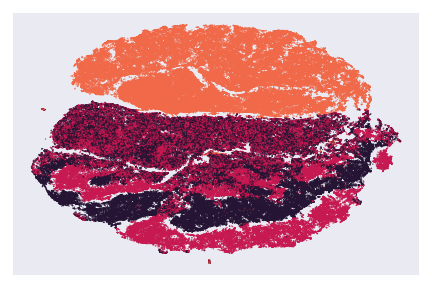
\includegraphics[width=0.25\textwidth]{images/tsne_z}}\\

\subcaptionbox{$L$\label{fig:tsne_lval}}{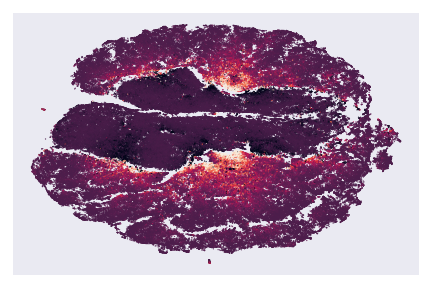
\includegraphics[width=0.25\textwidth]{images/tsne_lval}}\hfill
\subcaptionbox{$\xi$\label{fig:tsne_zL}}{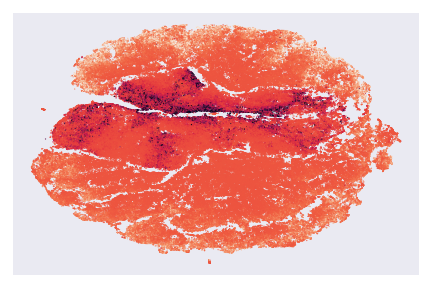
\includegraphics[width=0.25\textwidth]{images/tsne_zL}}\hfill
\subcaptionbox{$\partial\overline{u}/\partial{z}$\label{fig:tsne_dwdz}}{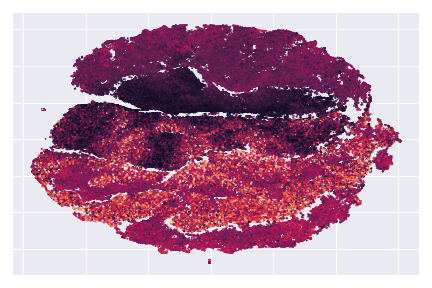
\includegraphics[width=0.25\textwidth]{images/tsne_dwdz}}\hfill
\subcaptionbox{$\phi_m$\label{fig:tsne_phi_m}}{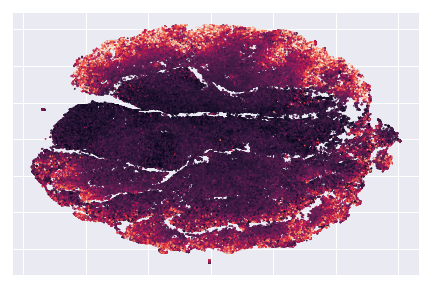
\includegraphics[width=0.25\textwidth]{images/tsne_phi_m}}\\

\subcaptionbox{$\partial\overline{\theta_v}/\partial{z}$\label{fig:tsne_dtdz}}{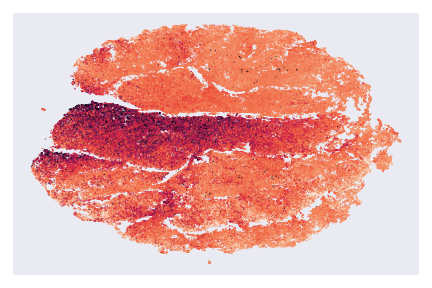
\includegraphics[width=0.25\textwidth]{images/tsne_dtdz}}\hfill
\subcaptionbox{Dew Point\label{fig:tsne_dewpoint}}{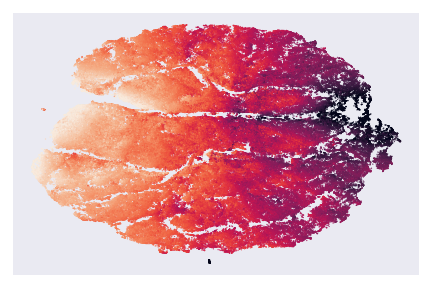
\includegraphics[width=0.25\textwidth]{images/tsne_dewpoint}}\hfill
\subcaptionbox{Spec. Hum.\label{fig:tsne_spec_hum}}{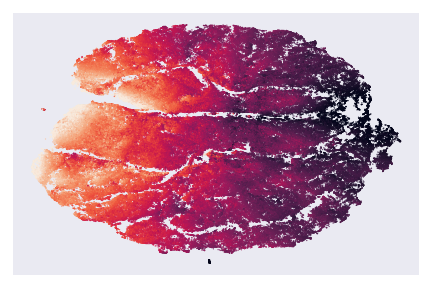
\includegraphics[width=0.25\textwidth]{images/tsne_spec_hum}}\hfill
\subcaptionbox{Rel. Hum.\label{fig:tsne_rel_hum}}{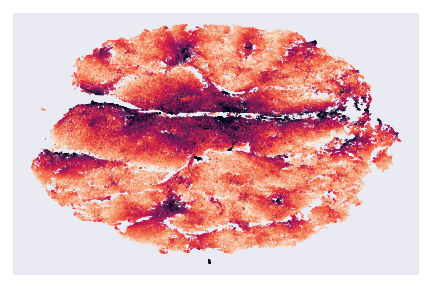
\includegraphics[width=0.25\textwidth]{images/tsne_rel_hum}}\\

\subcaptionbox{Air Pressure\label{fig:tsne_press}}{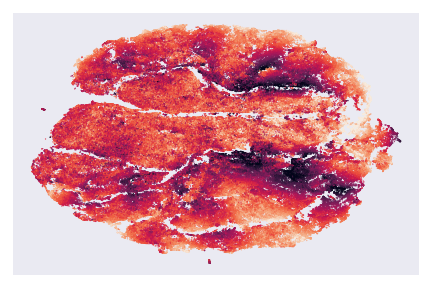
\includegraphics[width=0.25\textwidth]{images/tsne_press}}\hfill
\subcaptionbox{Rain\label{fig:tsne_rain}}{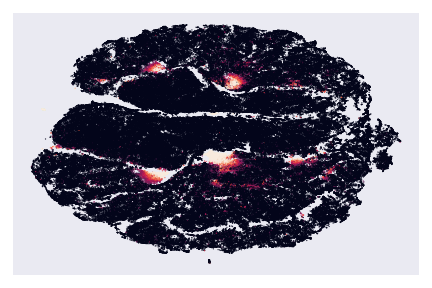
\includegraphics[width=0.25\textwidth]{images/tsne_rain}}\hfill
\subcaptionbox{$CO_2$ Flux\label{fig:tsne_co2flux}}{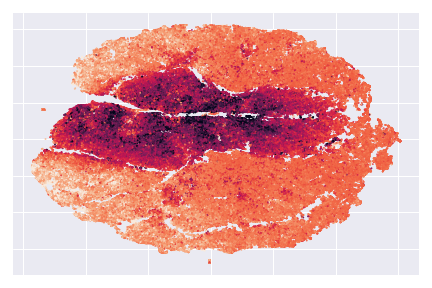
\includegraphics[width=0.25\textwidth]{images/tsne_co2flux}}\hfill
\subcaptionbox{Soil Heat Flux\label{fig:tsne_soilheat}}{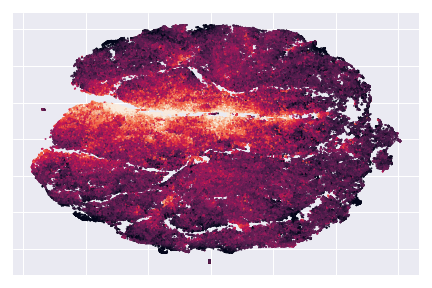
\includegraphics[width=0.25\textwidth]{images/tsne_soilheat}}\\

\subcaptionbox{Net Rad.\label{fig:tsne_netrad}}{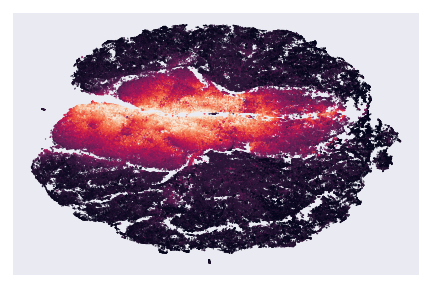
\includegraphics[width=0.25\textwidth]{images/tsne_netrad}}\hfill
\subcaptionbox{$\vert \text{Month}-6\vert$\label{fig:tsne_month}}{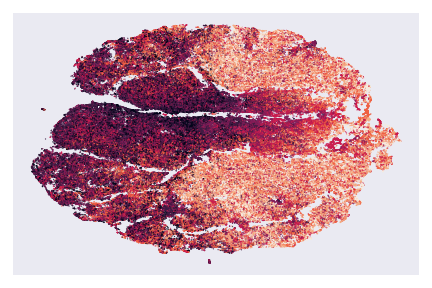
\includegraphics[width=0.25\textwidth]{images/tsne_month}}\hfill
\subcaptionbox{$\vert \text{Hr. Day}-12\vert$\label{fig:tsne_hday}}{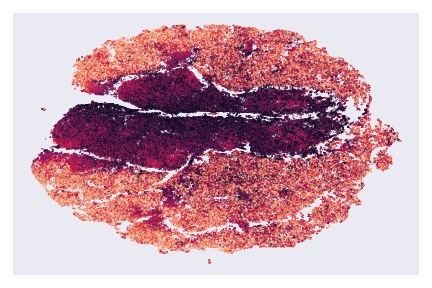
\includegraphics[width=0.25\textwidth]{images/tsne_hday}}\hfill
\subcaptionbox{k-Means\label{fig:tsne_clus}}{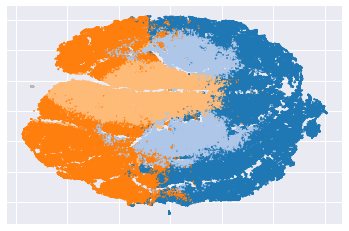
\includegraphics[width=0.25\textwidth]{images/tsne_clus}}\hfill

    \caption{Results of the t-SNE dimensionality reduction algorithm; every figure uses a different feature to color the points (darker points have smaller values), except figure \ref{fig:tsne_clus}, where the colors represent the result of 2-means clustering (blue/orange) and 4-means clustering (the four shades). The colors are consistent, in the sense that light and dark shades of blue are placed in the same cluster by 2-means clustering, ditto for orange. Figures \ref{fig:tsne_month} and \ref{fig:tsne_hday} use respectively the month and hour of day as feature values, but are colored using the values transformed with the formula in their caption. The points were drawn in random order. (Best viewed in color)}
	\label{fig:tsne}
\end{figure}


Talking about speed of wind, figure \ref{fig:ustar_wind} shows some measurements exceeding \SI{25}{\meter\per\second}; according to the Beaufort scale, holding umbrellas and walking become hard at \SI{15}{\meter\per\second}. Those measurements are not issues with the data: figure \ref{fig:cyclone_jeanett} shows the highest wind speed present in the Cesar database to date, corresponding to cyclone Jeanett.

\begin{figure}
    \centering
	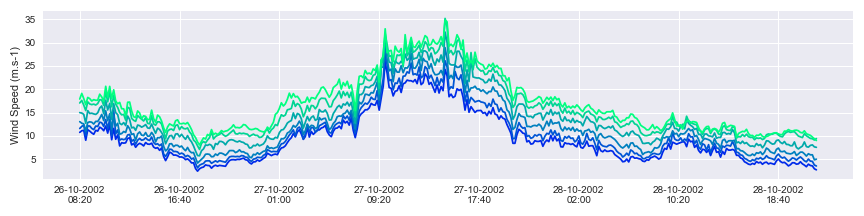
\includegraphics[width=0.95\textwidth]{images/cyclone_jeanett}
	\caption{Wind speed measurements during Cyclone Jeanett, which struck north-west Europe in October 2002, causing 33 fatalities. The top of the mast registered winds at \SI{35}{\meter\per\second}; although, in absolute terms, destructive, this cyclone registered winds up to \SI{42.5}{\meter\per\second} in other parts of Europe!}
	\label{fig:cyclone_jeanett}
\end{figure}



\section{Gradient Computation}
\label{sec:res_gradient}
Section \ref{sec:gradients} introduced three different ways to compute the gradient, but we need to choose one to compute the universal functions. In this section, we refer to the finite differences method in equation \ref{eq:fd_gradient} as \emph{FD}, the logarithm-based model of equation \ref{eq:log_gradient} as \emph{LG} and the Gaussian Process-based model of equation \ref{eq:gp_gradient} as \emph{GP}. Table \ref{tbl:gradients_corr} shows the Pearson correlation coefficient between the three methods, separately for every altitude level. It is clear that the FD gradient is inadequate at the lowest level; this can be explained by considering that equation \ref{eq:fd_gradient} with $z=10$ reduces to the wind speed at 20 meters divided by 20. This method appears to be too naive, especially since it does not take the roughness length into consideration, but, as \cite{cabauw_z0} showed, finding a value for $z_0$ is far from trivial. In spite of this, the FD and the Log gradients strongly agree on all levels, and are quite different from the gradients by GP

\begin{table}[]
\centering
\caption{Pearson correlation coefficient between the gradients predicted by the different methods, divided by level. The FD gradient is poorly correlated with the other two methods at the 10 meters level, but is very well correlated with the LG gradient at the other levels. The LG and GP gradients disagree on the lower levels, but it appears their predictions converge as altitude increases.}
\label{tbl:gradients_corr}
\begin{tabular}{c|c|c|c}
\toprule
\textbf{z} & \textbf{FD / GP} & \textbf{LG / FD} & \textbf{LG / GP} \\ \midrule
 	10 & 	0.192 & 0.480 &	0.317 \\
 	20 &	0.645 	& 0.991 &	0.640 \\
 	40 &	0.863 & 0.981 &	0.835 \\
\bottomrule
\end{tabular}
\end{table}

Since LG and GP. predict the wind speed too, we can compare their predictions to the measured wind speed. Notice that these methods are fitted on the wind speed at all levels, from 10 to 200 meters, but we evaluate them only on the three lowest levels, since that is where we compute the universal functions. Table \ref{tbl:model_wind_errors} shows the squared error between the modeled wind and the true wind speed at the three levels for both models. It is interesting to see that both models are quite accurate at all levels; this allows us to conclude that FD is not reliable at 10 meters.

\begin{table}[]
\centering
\caption{Absolute percent error of the wind speed modeled by the LG and GP methods at each altitude level. The altitude does not affect the error, and the GP wind speed is closer to the true wind speed than the LG model in the vast majority of cases, although the difference is negligible, often less than a few percents.}
\label{tbl:model_wind_errors}
\begin{tabular*}{\textwidth}{l @{\extracolsep{\fill}} |ccc|ccc|ccc}
\toprule
& \textbf{z} & \textbf{LG} & \textbf{GP} & \textbf{z} & \textbf{LG} & \textbf{GP} & \textbf{z} & \textbf{LG} & \textbf{GP} \\\midrule
\textbf{Mean} & \multirow{7}{*}{ 10 } & 1.2250 & 1.0329 & \multirow{7}{*}{ 20 } & 2.2605 & 1.4217 & \multirow{7}{*}{ 40 } & 1.3878 & 1.0364 \\
\textbf{Std.}& & 1.4033 & 1.1169 & & 2.3432 & 1.4658 & & 1.4783 & 1.1208 \\
\textbf{Min.} & & 0.0000 & 0.0000 & & 0.0000 & 0.0000 & & 0.0000 & 0.0000 \\
\textbf{25\%} & & 0.3714 & 0.3249 & & 0.7447 & 0.4549 & & 0.4744 & 0.3037 \\
\textbf{50\%} & & 0.8217 & 0.7608 & & 1.6251 & 1.0595 & & 1.0263 & 0.7265 \\
\textbf{75\%} & & 1.5505 & 1.4179 & & 2.9642 & 1.9693 & & 1.8413 & 1.4143 \\
\textbf{Max.} & & 53.7541 & 212.3985 & & 106.5623 & 192.9434 & & 80.3531 & 43.4657 \\
\bottomrule
\end{tabular*} 
\end{table}


Figure \ref{fig:gp_log_perc_err_wind_speed} shows the error as a function of the wind speed. It is interesting to see that GP becomes more and more reliable as the wind speed increases; not only does its error decrease, so does the variance of the error. It is possible to give an intuitive explanation for the error of LG: the measurement error of the wind speed is the maximum between \SI{0.1}{\meter\per\second} and 1\%, therefore the error of Log can be attributed almost entirely to uncertainty in the data, whereas GP seems to be overfitting.

\begin{figure}
    \centering
	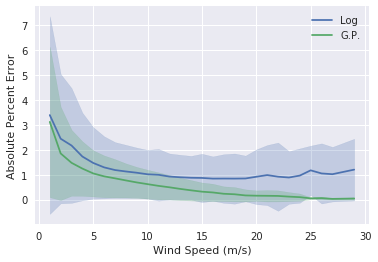
\includegraphics[width=0.6\textwidth]{images/gp_log_perc_err_wind_speed}
	\caption{Mean absolute percent error of the wind modeled by the LG and GP models as a function of the true wind speed; the lines are the average, and the shaded regions enclose the average plus or minus the standard deviation. Both quantities are computed by binning the wind by its integral part. Notice that slightly less than 5\% are above \SI{11}{\meter\per\second}, and only 656 observations, or 0.04\% of the total, are above \SI{20}{\meter\per\second} (\SI{72}{\kilo\meter\per\hour})}
	\label{fig:gp_log_perc_err_wind_speed}
\end{figure}


Given that the final goal of finding the gradient is to compute the universal functions, for which we already have more or less agreed upon expressions (equation \ref{eq:phi_m_coeff}), it makes sense to compare the error of these expressions when predicting the universal functions (equation \ref{eq:phi_m}) computed with the gradients coming from the three different methods; the best method is, then, the one with the smallest error. Table \ref{tbl:gradient_errors} contains these errors, both with all the data, and by considering only $2\leq\xi\leq 1$. FD is slightly better than LG if we do not consider the \SI{10}{\meter} level, but way worse if we include it. GP is significantly worse than FD in the MOST validity region, but only slightly worse on the whole dataset; this suggests that GP is weak when $\vert\xi\vert$ is small. 

\begin{table}[]
\centering
\caption{Mean squared error of $\phi_m$ (coefficients according to equation \ref{eq:phi_m_coeff}) when predicting the empirical flux-profile relationship (equation \ref{eq:phi_m}), computed with the three methods of calculating the gradient. The errors in second line (F.D. w/o z=10) were computed after discarding the data at the 10 meters level, because we argued the F.D. method is not reliable at that level. We show the error both in the range where the Monin-Obukhov similarity theory is known to be valid (84\% of the samples), and the error using all data.}
\label{tbl:gradient_errors}
\begin{tabular}{l|r|r}
\toprule
Method & MSE ($-2\leq\xi\leq1$) & MSE (full dataset) \\ \midrule
F.D. & 1.994 & 9.322 \\
F.D. (w/o z=10) & 0.627  & 11.832 \\
Log & 0.660 & 8.498 \\
G.P. & 1.213 & 8.899 \\
\bottomrule
\end{tabular}
\end{table}

To conclude, although FD (equation \ref{eq:fd_gradient}) is the most accurate way of computing the profile gradient, it does not allow us to use data at the \SI{10}{\meter} level. Considering that LG (equation \ref{eq:log_gradient}) is just slightly worse, but allows us to include that level (increasing the data available by 50\%!), all the results presented from now on make use of it.


\section{Flux-Profile Relationship}
\label{sec:most_res}
Figure \ref{fig:most_scatter} shows the wind shear versus the instability parameter, together with the commonly accepted flux-profile relationship in green and the relationship fitted on our dataset in red. Qualitatively, the scatter plot looks as expected, going to zero as $\xi$ decreases, linearly increasing in the $0\leq\xi\leq1$ interval, and leveling after that, possibly approaching the $\xi^{1/3}$ form proposed by \cite{sheba_phim}. In the next sections, we refer to the interval $-2\leq\xi\leq1$ as the \emph{MOST validity range}, or \emph{MOST dataset}; it contains 1,297,841 samples, 83.6\% of the total.

\begin{figure}
    \centering
    \begin{subfigure}[t]{0.49\textwidth}
        \centering
        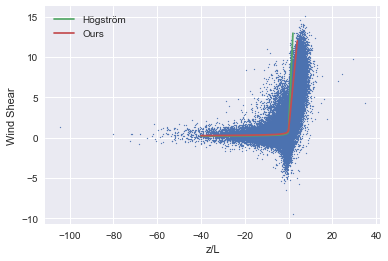
\includegraphics[width=\textwidth]{images/most_full}
        \caption{Full dataset}
        \label{fig:most_full}
    \end{subfigure}
    \hfill
    \begin{subfigure}[t]{0.49\textwidth}
        \centering
        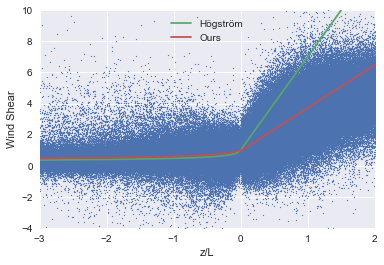
\includegraphics[width=\textwidth]{images/most_zoom}
        \caption{MOST Dataset}
        \label{fig:most_zoom}
    \end{subfigure}
    \caption{Wind shear $\phi_m$ versus the instability parameter $\xi$, with the prediction according to equation \ref{eq:phi_m_coeff} in green, and our predictions, following equation \ref{eq:phi_general} with the coefficients being the median values in table \ref{tbl:most_coeffs}, in red. Refer to the main text for a discussion of the difference.}
	\label{fig:most_scatter}
\end{figure}

\subsection{MOST Estimator}
The performance of the MOST estimator is shown in table \ref{tbl:most_results}; we see a considerable increase in the MSE when the full dataset is used; this is not surprising, considering that, with $\xi>1$, $\phi_m$ tends to level off, and there are a considerable number of outliers in the range $-20\leq\xi\leq-2$ (see figure \ref{fig:most_full}) that cannot be fitted by the MOST estimator. Figure \ref{fig:most_scatter} shows $\phi_m$ as a function of $\xi$ as computed in our dataset, as well as the predictions of equation \ref{eq:phi_m_coeff} and the fitted MOST estimator.
 
Table \ref{tbl:most_results} shows the values of the coefficients in equation \ref{eq:phi_general}, when fitted to the region of data where the Monin-Obukhov similarity theory is valid. We note a big difference with the values recommended in \cite{hogstrom88}, as well as most studies on the topic. However, \cite{cabauw_night_most} studied the stable, nocturnal boundary layer at Cabauw, and reported values varying between 0.81 and 0.95 for $a$ and between 2.7 and 3.2 for $b$, depending on the direction of the wind; there is no known explanation for this discrepancy. Although \cite{cabauw_night_most} used the same method that we applied to find the coefficients, no goodness of fit statistics, such as MSE or $R^2$, were reported.

\begin{table}[]
\centering
\caption{Evaluation metrics for the MOST estimator on both datasets obtained with nested cross-validation. The first number is the average over the 10 outer folds, followed by the standard deviation in parentheses.}
\label{tbl:most_results}
\centering\begin{tabular}{l|rr}
\toprule
{} &              All &            MOST \\
\midrule
\textbf{MSE  } &  0.64 (0.04) &  0.32 (0.02) \\
\textbf{$R^2$} &  0.71 (0.01) &  0.61 (0.01) \\
\textbf{MAE  } &  0.53 (0.01) &  0.39 (0.01) \\
\textbf{mAE  } &  0.37 (0.01) &  0.28 (0.01) \\
\textbf{MAPE } &  257.80 (207.39) &  178.68 (71.19) \\
\textbf{mAPE } &  28.48 (0.81) &  24.42 (0.84) \\
\bottomrule
\end{tabular}

\end{table}

\begin{table}[]
\centering
\caption{Values of the coefficients of the MOST estimator of equation \ref{eq:phi_general} fitted in the MOST validity range. The minimum values for $c$ and $d$ seem to be outliers, as well as the next smallest value, but the other 8 values are closely clustered together within an interval of about 0.15.}
\label{tbl:most_coeffs}
\begin{tabular}{r|rrrrrrr}
\toprule
   & \textbf{Mean} & \textbf{Std.} & \textbf{Min.} & \textbf{25\%} & \textbf{50\%} & \textbf{75\%} & \textbf{Max.} \\ \midrule
$a$ & 0.94 & 0.00 & 0.94 & 0.94 & 0.94 & 0.95 & 0.95 \\
$b$ & 2.77 & 0.01 & 2.76 & 2.77 & 2.77 & 2.78 & 2.78 \\
$c$ & 2.45 & 0.47 & 1.25 & 2.61 & 2.65 & 2.67 & 2.71 \\
$d$ & -0.30 & 0.11 & -0.60 & -0.26 & -0.26 & -0.26 & -0.25 \\
\bottomrule
\end{tabular}
\end{table}

\subsection{Other Estimators}
Table \ref{tbl:baseline_comparison} shows descriptive statistics of the MSE obtained by the best combination of features and trend, for each estimator and for each datasets, as well as the effect size comparing it with the MOST baseline. The scores were obtained with the nested cross validation procedure. The best combination of features and trend is the one with the largest lower bound of the 95\% CI; although in this case it equals the combination with the largest point estimate of the effect size, we feel that a definition in terms of the CI is more robust and reliable. It is very interesting to compare the kNN and GBT estimators: kNN manages to get a larger effect size when compared to MOST, despite the fact that its best performance corresponds to GBT's worst. This can be explained by the different scatter of the data points: kNN is more consistent, with only a couple of outliers driving up the standard deviation, while GBT's performances are more evenly scattered (and the rounding to two decimal digits in the table is deceiving). Consider the samples with the full dataset: the interquartile range for kNN is 0.025, whereas for GBT it is 0.055, and the Winsorized standard deviation over $10^4$ bootstraps is respectively 0.017 and 0.027. This difference is large enough to counteract the difference in means, and produce a larger effect size.

\begin{table}[p]
\caption{Descriptive statistics of the best MSE achieved by each estimator, and effect size comparing it (treatment) with the MOST baseline (control); the effect size is positive when the treatment has a lower MSE. The first number is the lower bound for the right 95\% CI interval, and the second number is the estimated population effect size; in bold are the CIs that do not contain 0. The only model which is not significantly better than the MOST baseline is Ridge on the MOST dataset.}
\label{tbl:baseline_comparison}
\setcellgapes{1ex}\makegapedcells\centering\begin{tabular*}{\textwidth}{cr|@{\extracolsep{\fill}}rrrrrrrr}
\toprule
     &      & \textbf{Mean} & \textbf{Std.} & \textbf{Min.} & \textbf{50\%} & \textbf{Max.} & \textbf{Effect Size} \\
\textbf{Dataset} & \textbf{Model} &               &               &               &               &               &                      \\
\midrule
\multirowcell{8}[3ex][c]{\textbf{Full}} & \textbf{MOST} &  0.64 &  0.04 &  0.58 &  0.63 &  0.71 &  - \\
     & \textbf{GB} &  0.36 &  0.03 &  0.31 &  0.37 &  0.40 &  \textbf{4.97/6.36} \\
     & \textbf{kNN} &  0.45 &  0.02 &  0.40 &  0.46 &  0.48 &  \textbf{4.78/9.44} \\
     & \textbf{Ridge} &  0.62 &  0.08 &  0.53 &  0.60 &  0.80 &  -0.06/0.55 \\
\cline{1-8}
\multirowcell{8}[3ex][c]{\textbf{MOST}} & \textbf{MOST} &  0.32 &  0.02 &  0.29 &  0.32 &  0.34 &  - \\
     & \textbf{GB} &  0.18 &  0.01 &  0.15 &  0.18 &  0.19 &  \textbf{7.52/10.98} \\
     & \textbf{kNN} &  0.25 &  0.01 &  0.22 &  0.25 &  0.25 &  \textbf{5.57/12.99} \\
     & \textbf{Ridge} &  0.27 &  0.02 &  0.24 &  0.27 &  0.29 &  \textbf{1.96/2.91} \\
\bottomrule
\end{tabular*}

\end{table}

\begin{table}[p]
\caption{Effect sizes comparing the MSE scores of each feature set with and without trend; the upper effect size uses the trend as treatment, whereas the lower effect size uses the trend as control. The first number is the lower bound for the right 95\% CI interval, and the second number is the estimated population effect size; positive effect size denotes improvement over the control group, in bold are the CIs that do not contain 0. Using the trend does not improve the performance.}
\label{tbl:trend_comparison}
\setcellgapes{1ex}\makegapedcells\centering\begin{tabular*}{\textwidth}{l @{\extracolsep{\fill}} c|ccccc}
\toprule
  & \textbf{Features} &                                  F1 &                                  F2 &                                  F3 &                                  F4 &                                  F5 \\
\textbf{MOST} & \textbf{Estimator} &                                     &                                     &                                     &                                     &                                     \\
\midrule
\multirowcell{6}[0.75ex][c]{\textbf{N}} & \textbf{GB} &  \makecell[c]{0.24\\(-0.68; 1.17)} &  \makecell[c]{0.21\\(-0.72; 1.13)} &  \makecell[c]{-0.48\\(-1.42; 0.47)} &  \makecell[c]{0.89\\(-0.09; 1.86)} &  \makecell[c]{-0.52\\(-1.47; 0.43)} \\
  & \textbf{Ridge} &  \makecell[c]{0.04\\(-0.89; 0.96)} &  \makecell[c]{-0.02\\(-0.94; 0.91)} &  \makecell[c]{-0.02\\(-0.95; 0.90)} &  \makecell[c]{-0.02\\(-0.95; 0.90)} &  \makecell[c]{-0.01\\(-0.94; 0.91)} \\
  & \textbf{kNN} &  \makecell[c]{-0.01\\(-0.93; 0.92)} &  \makecell[c]{-0.00\\(-0.93; 0.92)} &  \makecell[c]{0.10\\(-0.83; 1.02)} &  \makecell[c]{0.04\\(-0.89; 0.96)} &  \makecell[c]{-0.03\\(-0.95; 0.89)} \\
\cline{1-7}
\multirowcell{6}[0.75ex][c]{\textbf{Y}} & \textbf{GB} &  \makecell[c]{-0.06\\(-0.99; 0.86)} &  \makecell[c]{0.09\\(-0.84; 1.01)} &  \makecell[c]{0.76\\(-0.22; 1.73)} &  \makecell[c]{-0.24\\(-1.17; 0.68)} &  \makecell[c]{0.43\\(-0.51; 1.38)} \\
  & \textbf{Ridge} &  \makecell[c]{-0.05\\(-0.98; 0.87)} &  \makecell[c]{0.02\\(-0.91; 0.94)} &  \makecell[c]{0.02\\(-0.90; 0.94)} &  \makecell[c]{-0.02\\(-0.94; 0.90)} &  \makecell[c]{0.05\\(-0.87; 0.97)} \\
  & \textbf{kNN} &  \makecell[c]{-0.06\\(-0.98; 0.87)} &  \makecell[c]{-0.02\\(-0.94; 0.91)} &  \makecell[c]{0.12\\(-0.81; 1.04)} &  \makecell[c]{0.15\\(-0.77; 1.08)} &  \makecell[c]{0.02\\(-0.90; 0.94)} \\
\bottomrule
\end{tabular*}

\end{table}

\begin{table}[p]
\caption{Effect sizes comparing the MSE scores of all pairs of feature sets; in light of table \ref{tbl:trend_comparison}, the trend is not included in the features. The control is on rows, and the treatment is on columns. The first number is the lower bound for the right 95\% CI interval, and the second number is the estimated population effect size; positive effect size denotes improvement over the control group, in bold are the CIs that do not contain 0. The only feature sets that do not bring an improvement are F2 over F1 and F4 over F3.}
\label{tbl:fset_comparison}
\setcellgapes{1ex}\makegapedcells\centering\begin{tabular*}{\textwidth}{ccc|@{\extracolsep{\fill}}cccc}
\toprule
     &     &    & \textbf{F2} &       \textbf{F3} &       \textbf{F4} &       \textbf{F5} \\
\textbf{Dataset} & \textbf{Model} & \textbf{Features} &             &                   &                   &                   \\
\midrule
\multirowcell{10}[4ex][c]{\textbf{MOST}} & \multirowcell{10}[4ex][c]{\textbf{GBT}} & \textbf{F1} &  -0.2/0.2 &  \textbf{0.5/1.0} &  \textbf{0.2/0.7} &  \textbf{1.6/2.5} \\
     &     & \textbf{F2} &  - &  \textbf{0.5/0.8} &  \textbf{0.1/0.6} &  \textbf{1.5/2.3} \\
     &     & \textbf{F3} &  - &  - &  -0.9/-0.4 &  \textbf{0.4/1.0} \\
     &     & \textbf{F4} &  - &  - &  - &  \textbf{0.8/1.4} \\
     &     & \textbf{F5} &  - &  - &  - &  - \\
\bottomrule
\end{tabular*}

\end{table}

The scores used to perform the comparisons in tables \ref{tbl:trend_comparison} and \ref{tbl:fset_comparison} were obtained by repeating the cross validation procedure 5 times.

Table \ref{tbl:trend_comparison} compares each feature set with and without trend, for the MOST dataset and the GBT estimator. Essentially, the table shows that the features augmented with trend do not provide a significant improvement over those without trend; it is interesting to relate this result with table \ref{tbl:baseline_comparison}, where the largest effect size when comparing GBT with MOST is actually obtained with the trend. This is another example of differing standard deviations counteracting the difference in means.

Table \ref{tbl:fset_comparison} compares every pair of feature set, again restricted to the MOST dataset and the GBT estimator. Given that the trend does not provide additional benefits, we compare the feature sets without the trend. The only feature sets that do not improve over the previous sets are F2 (soil heat flux) over F1 and F4 (rain amount and dew point) over F3; in all other cases, adding features gives a significant improvement.

\chapter{Discussion}
\label{ch:discussion}
As shown in table \ref{tbl:baseline_comparison}, we could improve the predictions of the similarity theory even with a simple regularized linear model. Furthermore, \ref{tbl:trend_comparison} shows that no useful information can be obtained from knowing the value of a feature one hour earlier than the prediction. Finally, table \ref{tbl:fset_comparison} shows that, besides the heat fluxes, the net radiation is an important predictor, whereas the dew point and the soil heat flux do not contribute significantly to the predictive performance.



\subsection{Features}
 Of course, we cannot rule out the possibility that the model was able to figure out the information contained in these features, thus making them redundant, or needed other features to make sense of them.
 
 
actual constants and coefficients (e.g. von karmans constant) dont really matter, because they are constant and do not affect the ml model (can be figured out)

estimating parameters (von karman, roughness length etc) is very difficult, by using ml we can circumvent the problem (they need a supporting infrastructure even if they want to compute those constants, so not huge downside)



one of the reasons why MOST is unreliable in stable conditions is because of the difficulty of measuring fluxes. there are other methods to compute the turbulent fluxes (http://bibliotheek.knmi.nl/knmipubWR/WR87-02.pdf, ), we used eddy corr because that's what in the cesar database

wind direction is very important since different characteristics of the surface affect the measurements, see https://journals.ametsoc.org/doi/full/10.1175/2006JAMC1298.1 and somebody else on cabauw

our models can only be used in conditions that are similar to cabauw. most importantly, they are not valid in the oceanic surface layer, because it is very different [citation]

richardson number instead of obukhov length


trend could be better included using some sort of time series prediction together with the features we considered in this work, but preliminary experiments (3 layers gru + 4 layers fully connected) do not seem to work well)


generalization problem: surface roughness? simulations already use some parameters for this

\paragraph{Samples}
outliers with xi between -20 and -2 mostly belong to z=40 in the morning (between 6 and 12); given what was said in [paper], there is the possibility that they are not in the surface layer, explaining why the c coefficient is higher than expected


can generate new training samples at more altitude levels, since we have a model for wind and temp (need to interpolate spec. humidity too), according to the simulation that uses this model


\paragraph{Performance}
This is a notable achievement, since the chosen model will be just one of the many components of climate simulations, which are notoriously very slow and computationally intensive. A linear model has the potential to compete with the efficiency of MOST, depending on the number of features, since it is fundamentally a dot product

even though we predicted phim, the actual interest is in u*. we predict phim to have a direct means of comparing with state of the art (?), \cite{weber1999} computes u* from the standard deviations obtaining rmse between 0.05 and 0.1



incorporate uncertainty in the model (e.g. quantile regression), then use this in the simulations to get climate uncertainty (monte carlo by sampling from prediction would be a quick and dirty way of implementing this, although it would make the simulation quite slow)

defense thu 14 at 11 in kista room grottan

ask ying to review my thesis

seems like it's fairly new, no ML attempts

boundary layer journal


\section{Limitations and Future Work}
todo

\appendix
\chapter{Detailed Results}
\label{apx:all_results}
The averaged evaluation metrics for the Ridge, kNN and GBT estimators are presented in tables \ref{tbl:ridge_results}, \ref{tbl:knn_results}
and \ref{tbl:gbr_results}, while figures \ref{fig:ridge_results_most}, \ref{fig:knn_results_most} and \ref{fig:gbr_results_most} show boxplots of these metrics for the MOST validity range, and figures \ref{fig:ridge_results_all}, \ref{fig:knn_results_all} and \ref{fig:gbr_results_all} do so for the whole dataset. Finally, tables \ref{tbl:params_ridge}, \ref{tbl:params_knn} and \ref{tbl:params_gbt} list the hyper-parameters obtained in each outer fold that generated the best results shown in table \ref{tbl:baseline_comparison}.

\begin{figure}[h]
\subcaptionbox{Mean Squared Error\label{fig:result_Ridge_most_mean_squared_error}}{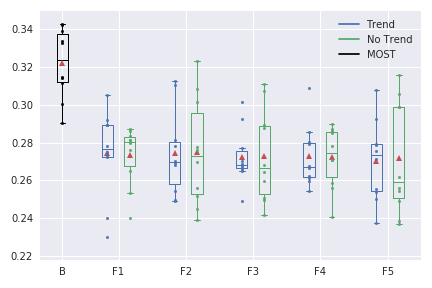
\includegraphics[width=0.5\textwidth]{images/result_Ridge_most_mean_squared_error}}\hfill
\subcaptionbox{$R^2$ Score \label{fig:result_Ridge_most_r2_score}}{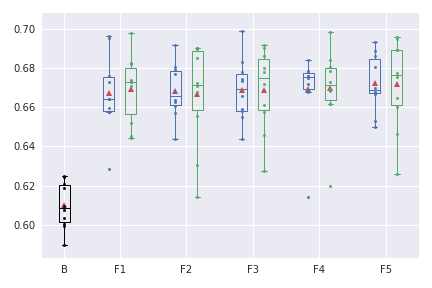
\includegraphics[width=0.49\textwidth]{images/result_Ridge_most_r2_score}}\\

\subcaptionbox{Mean Absolute Error\label{fig:result_Ridge_most_mean_absolute_error}}{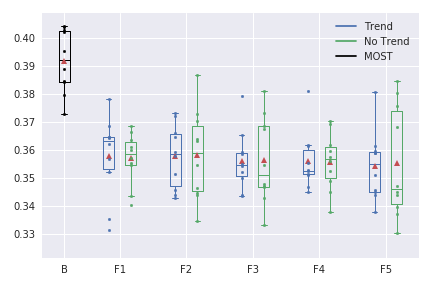
\includegraphics[width=0.49\textwidth]{images/result_Ridge_most_mean_absolute_error}}
\subcaptionbox{Median Absolute Error\label{fig:result_Ridge_most_median_absolute_error}}{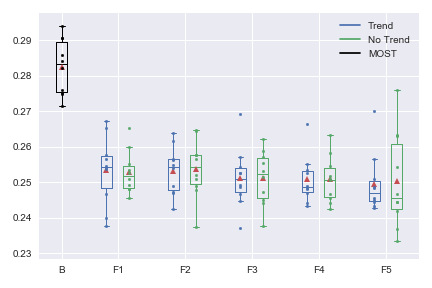
\includegraphics[width=0.49\textwidth]{images/result_Ridge_most_median_absolute_error}}\\

\subcaptionbox{Mean Absolute Percent Error\label{fig:result_Ridge_most_mean_abs_percent_error}}{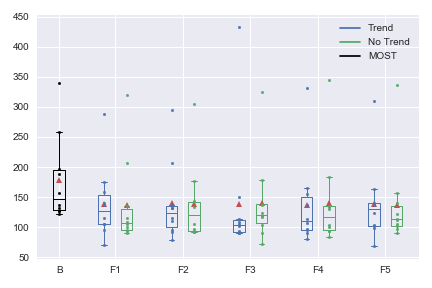
\includegraphics[width=0.49\textwidth]{images/result_Ridge_most_mean_abs_percent_error}}\hfill
\subcaptionbox{Median Absolute Percent Error\label{fig:result_Ridge_most_median_abs_percent_error}}{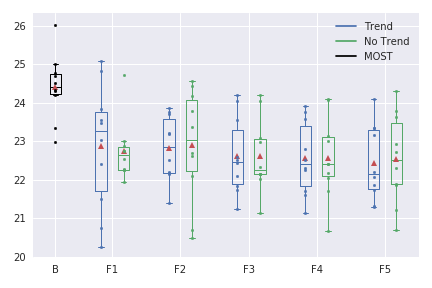
\includegraphics[width=0.49\textwidth]{images/result_Ridge_most_median_abs_percent_error}}\\

    \caption{Evaluation metrics of the Ridge Regression Estimator in the MOST validity range; the feature sets with trend are blue, those without trend are green, and he leftmost black box is the MOST estimator baseline.}
	\label{fig:ridge_results_most}
\end{figure}


\begin{figure}[h]
\subcaptionbox{Mean Squared Error\label{fig:result_Ridge_nomost_mean_squared_error}}{\includegraphics[width=0.5\textwidth]{images/result_Ridge_nomost_mean_squared_error}}\hfill
\subcaptionbox{$R^2$ Score \label{fig:result_Ridge_nomost_r2_score}}{\includegraphics[width=0.49\textwidth]{images/result_Ridge_nomost_r2_score}}\\

\subcaptionbox{Mean Absolute Error\label{fig:result_Ridge_nomost_mean_absolute_error}}{\includegraphics[width=0.49\textwidth]{images/result_Ridge_nomost_mean_absolute_error}}
\subcaptionbox{Median Absolute Error\label{fig:result_Ridge_nomost_median_absolute_error}}{\includegraphics[width=0.49\textwidth]{images/result_Ridge_nomost_median_absolute_error}}\\

\subcaptionbox{Mean Absolute Percent Error\label{fig:result_Ridge_nomost_mean_abs_percent_error}}{\includegraphics[width=0.49\textwidth]{images/result_Ridge_nomost_mean_abs_percent_error}}\hfill
\subcaptionbox{Median Absolute Percent Error\label{fig:result_Ridge_nomost_median_abs_percent_error}}{\includegraphics[width=0.49\textwidth]{images/result_Ridge_nomost_median_abs_percent_error}}\\

    \caption{Evaluation metrics of the Ridge Regression Estimator on all the data; the feature sets with trend are blue, those without trend are green, and he leftmost black box is the MOST estimator baseline.}
	\label{fig:ridge_results_all}
\end{figure}


\begin{table}[h]
\caption{Evaluation metrics for the Ridge estimator. }
\label{tbl:ridge_results}
\setcellgapes{0.15ex}\makegapedcells\centering\begin{tabular*}{\textwidth}{lcc|@{\extracolsep{\fill}}ccccc}
\toprule
    &      &   &                     \textbf{F1} &                     \textbf{F2} &                     \textbf{F3} &                     \textbf{F4} &                     \textbf{F5} \\
\textbf{Metric} & \textbf{Dataset} & \textbf{Trend} &                                 &                                 &                                 &                                 &                                 \\
\midrule
\multirowcell{8}[0.75ex][c]{\textbf{MSE}} & \multirowcell{4}[0.75ex][c]{\textbf{Full}} & \textbf{N} &  \makecell[c]{0.63\\(0.05)} &  \makecell[c]{0.63\\(0.07)} &  \makecell[c]{0.62\\(0.04)} &  \makecell[c]{0.63\\(0.06)} &  \makecell[c]{0.62\\(0.08)} \\
    &      & \textbf{Y} &  \makecell[c]{0.63\\(0.05)} &  \makecell[c]{0.63\\(0.07)} &  \makecell[c]{0.63\\(0.07)} &  \makecell[c]{0.63\\(0.08)} &  \makecell[c]{0.62\\(0.08)} \\
\cline{2-8}
    & \multirowcell{4}[0.75ex][c]{\textbf{MOST}} & \textbf{N} &  \makecell[c]{0.27\\(0.02)} &  \makecell[c]{0.27\\(0.03)} &  \makecell[c]{0.27\\(0.02)} &  \makecell[c]{0.27\\(0.02)} &  \makecell[c]{0.27\\(0.03)} \\
    &      & \textbf{Y} &  \makecell[c]{0.27\\(0.02)} &  \makecell[c]{0.27\\(0.02)} &  \makecell[c]{0.27\\(0.01)} &  \makecell[c]{0.27\\(0.02)} &  \makecell[c]{0.27\\(0.02)} \\
\hline
\multirowcell{8}[0.75ex][c]{\textbf{$R^2$}} & \multirowcell{4}[0.75ex][c]{\textbf{Full}} & \textbf{N} &  \makecell[c]{0.72\\(0.02)} &  \makecell[c]{0.72\\(0.02)} &  \makecell[c]{0.72\\(0.02)} &  \makecell[c]{0.72\\(0.02)} &  \makecell[c]{0.73\\(0.02)} \\
    &      & \textbf{Y} &  \makecell[c]{0.72\\(0.02)} &  \makecell[c]{0.72\\(0.03)} &  \makecell[c]{0.72\\(0.02)} &  \makecell[c]{0.72\\(0.03)} &  \makecell[c]{0.72\\(0.04)} \\
\cline{2-8}
    & \multirowcell{4}[0.75ex][c]{\textbf{MOST}} & \textbf{N} &  \makecell[c]{0.67\\(0.02)} &  \makecell[c]{0.67\\(0.03)} &  \makecell[c]{0.67\\(0.02)} &  \makecell[c]{0.67\\(0.02)} &  \makecell[c]{0.67\\(0.02)} \\
    &      & \textbf{Y} &  \makecell[c]{0.67\\(0.02)} &  \makecell[c]{0.67\\(0.01)} &  \makecell[c]{0.67\\(0.02)} &  \makecell[c]{0.67\\(0.02)} &  \makecell[c]{0.67\\(0.01)} \\
\hline
\multirowcell{8}[0.75ex][c]{\textbf{MAE}} & \multirowcell{4}[0.75ex][c]{\textbf{Full}} & \textbf{N} &  \makecell[c]{0.53\\(0.02)} &  \makecell[c]{0.53\\(0.03)} &  \makecell[c]{0.52\\(0.02)} &  \makecell[c]{0.52\\(0.02)} &  \makecell[c]{0.52\\(0.03)} \\
    &      & \textbf{Y} &  \makecell[c]{0.53\\(0.02)} &  \makecell[c]{0.53\\(0.02)} &  \makecell[c]{0.52\\(0.03)} &  \makecell[c]{0.52\\(0.03)} &  \makecell[c]{0.52\\(0.03)} \\
\cline{2-8}
    & \multirowcell{4}[0.75ex][c]{\textbf{MOST}} & \textbf{N} &  \makecell[c]{0.36\\(0.01)} &  \makecell[c]{0.36\\(0.02)} &  \makecell[c]{0.36\\(0.02)} &  \makecell[c]{0.36\\(0.01)} &  \makecell[c]{0.36\\(0.02)} \\
    &      & \textbf{Y} &  \makecell[c]{0.36\\(0.01)} &  \makecell[c]{0.36\\(0.01)} &  \makecell[c]{0.36\\(0.01)} &  \makecell[c]{0.36\\(0.01)} &  \makecell[c]{0.35\\(0.01)} \\
\hline
\multirowcell{8}[0.75ex][c]{\textbf{mAE}} & \multirowcell{4}[0.75ex][c]{\textbf{Full}} & \textbf{N} &  \makecell[c]{0.36\\(0.01)} &  \makecell[c]{0.36\\(0.02)} &  \makecell[c]{0.35\\(0.01)} &  \makecell[c]{0.35\\(0.01)} &  \makecell[c]{0.35\\(0.01)} \\
    &      & \textbf{Y} &  \makecell[c]{0.36\\(0.01)} &  \makecell[c]{0.36\\(0.01)} &  \makecell[c]{0.35\\(0.01)} &  \makecell[c]{0.35\\(0.01)} &  \makecell[c]{0.35\\(0.02)} \\
\cline{2-8}
    & \multirowcell{4}[0.75ex][c]{\textbf{MOST}} & \textbf{N} &  \makecell[c]{0.25\\(0.01)} &  \makecell[c]{0.25\\(0.01)} &  \makecell[c]{0.25\\(0.01)} &  \makecell[c]{0.25\\(0.01)} &  \makecell[c]{0.25\\(0.01)} \\
    &      & \textbf{Y} &  \makecell[c]{0.25\\(0.01)} &  \makecell[c]{0.25\\(0.01)} &  \makecell[c]{0.25\\(0.01)} &  \makecell[c]{0.25\\(0.01)} &  \makecell[c]{0.25\\(0.01)} \\
\hline
\multirowcell{8}[0.75ex][c]{\textbf{MAPE}} & \multirowcell{4}[0.75ex][c]{\textbf{Full}} & \textbf{N} &  \makecell[c]{262.89\\(258.33)} &  \makecell[c]{258.83\\(235.59)} &  \makecell[c]{269.43\\(278.64)} &  \makecell[c]{278.46\\(368.15)} &  \makecell[c]{262.95\\(252.08)} \\
    &      & \textbf{Y} &  \makecell[c]{262.27\\(271.17)} &  \makecell[c]{253.28\\(222.37)} &  \makecell[c]{268.17\\(314.75)} &  \makecell[c]{270.60\\(265.59)} &  \makecell[c]{261.74\\(270.25)} \\
\cline{2-8}
    & \multirowcell{4}[0.75ex][c]{\textbf{MOST}} & \textbf{N} &  \makecell[c]{137.37\\(73.04)} &  \makecell[c]{138.23\\(65.42)} &  \makecell[c]{140.78\\(70.93)} &  \makecell[c]{140.17\\(77.45)} &  \makecell[c]{137.71\\(72.83)} \\
    &      & \textbf{Y} &  \makecell[c]{139.18\\(60.62)} &  \makecell[c]{139.73\\(65.11)} &  \makecell[c]{137.92\\(104.84)} &  \makecell[c]{137.57\\(73.89)} &  \makecell[c]{138.81\\(66.28)} \\
\hline
\multirowcell{8}[0.75ex][c]{\textbf{mAPE}} & \multirowcell{4}[0.75ex][c]{\textbf{Full}} & \textbf{N} &  \makecell[c]{29.27\\(1.25)} &  \makecell[c]{29.30\\(1.63)} &  \makecell[c]{28.55\\(0.83)} &  \makecell[c]{28.56\\(1.32)} &  \makecell[c]{28.23\\(1.64)} \\
    &      & \textbf{Y} &  \makecell[c]{29.28\\(0.78)} &  \makecell[c]{29.34\\(1.55)} &  \makecell[c]{28.53\\(0.92)} &  \makecell[c]{28.60\\(1.42)} &  \makecell[c]{28.21\\(1.43)} \\
\cline{2-8}
    & \multirowcell{4}[0.75ex][c]{\textbf{MOST}} & \textbf{N} &  \makecell[c]{22.74\\(0.77)} &  \makecell[c]{22.90\\(1.46)} &  \makecell[c]{22.63\\(0.95)} &  \makecell[c]{22.58\\(1.05)} &  \makecell[c]{22.54\\(1.17)} \\
    &      & \textbf{Y} &  \makecell[c]{22.87\\(1.63)} &  \makecell[c]{22.81\\(0.85)} &  \makecell[c]{22.62\\(1.00)} &  \makecell[c]{22.56\\(0.96)} &  \makecell[c]{22.45\\(0.98)} \\
\bottomrule
\end{tabular*}

\end{table}


\begin{sidewaystable}
\caption{Hyper-parameters and MSE for each outer fold obtained by the best combination of trend and features in each dataset by the Ridge estimator.}
\label{tbl:params_ridge}
\setcellgapes{1ex}\makegapedcells\centering\begin{tabular}{cr|rrrrrrrrrr}
\toprule
     &       & \textbf{1} & \textbf{2} & \textbf{3} & \textbf{4} & \textbf{5} & \textbf{6} & \textbf{7} & \textbf{8} & \textbf{9} & \textbf{10} \\
\textbf{Dataset} & \textbf{H.P.} &            &            &            &            &            &            &            &            &            &             \\
\midrule
\multirowcell{4}[2ex][c]{\textbf{MOST}} & \textbf{(MSE)} &  0.304 &  0.285 &  0.285 &  0.280 &  0.284 &  0.281 &  0.258 &  0.236 &  0.243 &  0.276 \\
     & \textbf{Alpha} &  6.967 &  5.465 &  6.998 &  3.642 &  3.207 &  3.936 &  2.826 &  4.590 &  4.248 &  2.014 \\
\bottomrule
\end{tabular}

\end{sidewaystable}



% ---------------------------------------------------------------

\begin{figure}[h]
\subcaptionbox{Mean Squared Error\label{fig:result_KNeighborsRegressor_most_mean_squared_error}}{\includegraphics[width=0.49\textwidth]{images/result_kNN_most_mean_squared_error}}\hfill
\subcaptionbox{$R^2$ Score \label{fig:result_kNN_most_r2_score}}{\includegraphics[width=0.49\textwidth]{images/result_kNN_most_r2_score}}\\

\subcaptionbox{Mean Absolute Error\label{fig:result_kNN_most_mean_absolute_error}}{\includegraphics[width=0.49\textwidth]{images/result_kNN_most_mean_absolute_error}}
\subcaptionbox{Median Absolute Error\label{fig:result_kNN_most_median_absolute_error}}{\includegraphics[width=0.49\textwidth]{images/result_kNN_most_median_absolute_error}}\\

\subcaptionbox{Mean Absolute Percent Error\label{fig:result_kNN_most_mean_abs_percent_error}}{\includegraphics[width=0.49\textwidth]{images/result_kNN_most_mean_abs_percent_error}}\hfill
\subcaptionbox{Median Absolute Percent Error\label{fig:result_kNN_most_median_abs_percent_error}}{\includegraphics[width=0.49\textwidth]{images/result_kNN_most_median_abs_percent_error}}\\

    \caption{Evaluation metrics of the k-Nearest Neighbors Regressor Estimator in the MOST validity range; the feature sets with trend are blue, those without trend are green, and he leftmost black box is the MOST estimator baseline.}
	\label{fig:knn_results_most}
\end{figure}


\begin{figure}[h]
\subcaptionbox{Mean Squared Error\label{fig:result_kNN_nomost_mean_squared_error}}{\includegraphics[width=0.49\textwidth]{images/result_kNN_nomost_mean_squared_error}}\hfill
\subcaptionbox{$R^2$ Score \label{fig:result_kNN_nomost_r2_score}}{\includegraphics[width=0.49\textwidth]{images/result_kNN_nomost_r2_score}}\\

\subcaptionbox{Mean Absolute Error\label{fig:result_kNN_nomost_mean_absolute_error}}{\includegraphics[width=0.49\textwidth]{images/result_kNN_nomost_mean_absolute_error}}
\subcaptionbox{Median Absolute Error\label{fig:result_kNN_nomost_median_absolute_error}}{\includegraphics[width=0.49\textwidth]{images/result_kNN_nomost_median_absolute_error}}\\

\subcaptionbox{Mean Absolute Percent Error\label{fig:result_kNN_nomost_mean_abs_percent_error}}{\includegraphics[width=0.49\textwidth]{images/result_kNN_nomost_mean_abs_percent_error}}\hfill
\subcaptionbox{Median Absolute Percent Error\label{fig:result_kNN_nomost_median_abs_percent_error}}{\includegraphics[width=0.49\textwidth]{images/result_kNN_nomost_median_abs_percent_error}}\\

    \caption{Evaluation metrics of the k-Nearest Neighbors Regressor Estimator on all the data; the feature sets with trend are blue, those without trend are green, and he leftmost black box is the MOST estimator baseline.}
	\label{fig:knn_results_all}
\end{figure}


\begin{table}[h]
\caption{Evaluation metrics for the k-Nearest Neighbors estimator.}
\label{tbl:knn_results}
\setcellgapes{0.15ex}\makegapedcells\centering\begin{tabular*}{\textwidth}{l @{\extracolsep{\fill}} cc|ccccc}
\toprule
    &   & \textbf{Features} &                              F1 &                              F2 &                             F3 &                             F4 &                             F5 \\
\textbf{Metric} & \textbf{MOST} & \textbf{Trend} &                                 &                                 &                                &                                &                                \\
\midrule
\multirowcell{8}[0.75ex][c]{\textbf{MSE}} & \multirowcell{4}[0.75ex][c]{\textbf{N}} & \textbf{N} &  \makecell[c]{0.45\\(0.05)} &  \makecell[c]{0.48\\(0.04)} &  \makecell[c]{0.46\\(0.04)} &  \makecell[c]{0.49\\(0.04)} &  \makecell[c]{0.46\\(0.05)} \\
    &   & \textbf{Y} &  \makecell[c]{0.45\\(0.02)} &  \makecell[c]{0.48\\(0.03)} &  \makecell[c]{0.46\\(0.03)} &  \makecell[c]{0.49\\(0.04)} &  \makecell[c]{0.46\\(0.05)} \\
\cline{2-8}
    & \multirowcell{4}[0.75ex][c]{\textbf{Y}} & \textbf{N} &  \makecell[c]{0.22\\(0.01)} &  \makecell[c]{0.25\\(0.01)} &  \makecell[c]{0.24\\(0.02)} &  \makecell[c]{0.25\\(0.01)} &  \makecell[c]{0.25\\(0.02)} \\
    &   & \textbf{Y} &  \makecell[c]{0.23\\(0.02)} &  \makecell[c]{0.25\\(0.02)} &  \makecell[c]{0.24\\(0.02)} &  \makecell[c]{0.25\\(0.02)} &  \makecell[c]{0.25\\(0.02)} \\
\hline
\multirowcell{8}[0.75ex][c]{\textbf{$R^2$}} & \multirowcell{4}[0.75ex][c]{\textbf{N}} & \textbf{N} &  \makecell[c]{0.80\\(0.01)} &  \makecell[c]{0.79\\(0.01)} &  \makecell[c]{0.79\\(0.01)} &  \makecell[c]{0.78\\(0.01)} &  \makecell[c]{0.79\\(0.01)} \\
    &   & \textbf{Y} &  \makecell[c]{0.80\\(0.01)} &  \makecell[c]{0.79\\(0.01)} &  \makecell[c]{0.80\\(0.01)} &  \makecell[c]{0.78\\(0.01)} &  \makecell[c]{0.79\\(0.01)} \\
\cline{2-8}
    & \multirowcell{4}[0.75ex][c]{\textbf{Y}} & \textbf{N} &  \makecell[c]{0.73\\(0.01)} &  \makecell[c]{0.70\\(0.01)} &  \makecell[c]{0.71\\(0.01)} &  \makecell[c]{0.69\\(0.01)} &  \makecell[c]{0.69\\(0.01)} \\
    &   & \textbf{Y} &  \makecell[c]{0.73\\(0.01)} &  \makecell[c]{0.70\\(0.01)} &  \makecell[c]{0.71\\(0.01)} &  \makecell[c]{0.70\\(0.01)} &  \makecell[c]{0.70\\(0.01)} \\
\hline
\multirowcell{8}[0.75ex][c]{\textbf{MAE}} & \multirowcell{4}[0.75ex][c]{\textbf{N}} & \textbf{N} &  \makecell[c]{0.41\\(0.02)} &  \makecell[c]{0.43\\(0.02)} &  \makecell[c]{0.42\\(0.02)} &  \makecell[c]{0.43\\(0.01)} &  \makecell[c]{0.43\\(0.02)} \\
    &   & \textbf{Y} &  \makecell[c]{0.41\\(0.01)} &  \makecell[c]{0.43\\(0.01)} &  \makecell[c]{0.42\\(0.02)} &  \makecell[c]{0.43\\(0.02)} &  \makecell[c]{0.43\\(0.02)} \\
\cline{2-8}
    & \multirowcell{4}[0.75ex][c]{\textbf{Y}} & \textbf{N} &  \makecell[c]{0.31\\(0.01)} &  \makecell[c]{0.33\\(0.01)} &  \makecell[c]{0.32\\(0.01)} &  \makecell[c]{0.34\\(0.01)} &  \makecell[c]{0.34\\(0.01)} \\
    &   & \textbf{Y} &  \makecell[c]{0.31\\(0.01)} &  \makecell[c]{0.33\\(0.01)} &  \makecell[c]{0.32\\(0.01)} &  \makecell[c]{0.33\\(0.01)} &  \makecell[c]{0.34\\(0.01)} \\
\hline
\multirowcell{8}[0.75ex][c]{\textbf{mAE}} & \multirowcell{4}[0.75ex][c]{\textbf{N}} & \textbf{N} &  \makecell[c]{0.23\\(0.01)} &  \makecell[c]{0.25\\(0.01)} &  \makecell[c]{0.25\\(0.01)} &  \makecell[c]{0.26\\(0.01)} &  \makecell[c]{0.26\\(0.01)} \\
    &   & \textbf{Y} &  \makecell[c]{0.23\\(0.01)} &  \makecell[c]{0.25\\(0.01)} &  \makecell[c]{0.25\\(0.01)} &  \makecell[c]{0.26\\(0.01)} &  \makecell[c]{0.26\\(0.01)} \\
\cline{2-8}
    & \multirowcell{4}[0.75ex][c]{\textbf{Y}} & \textbf{N} &  \makecell[c]{0.20\\(0.01)} &  \makecell[c]{0.22\\(0.01)} &  \makecell[c]{0.22\\(0.01)} &  \makecell[c]{0.23\\(0.01)} &  \makecell[c]{0.23\\(0.01)} \\
    &   & \textbf{Y} &  \makecell[c]{0.20\\(0.01)} &  \makecell[c]{0.22\\(0.01)} &  \makecell[c]{0.22\\(0.01)} &  \makecell[c]{0.23\\(0.01)} &  \makecell[c]{0.23\\(0.01)} \\
\hline
\multirowcell{8}[0.75ex][c]{\textbf{MAPE}} & \multirowcell{4}[0.75ex][c]{\textbf{N}} & \textbf{N} &  \makecell[c]{149.67\\(128.39)} &  \makecell[c]{162.01\\(104.52)} &  \makecell[c]{158.82\\(88.71)} &  \makecell[c]{163.85\\(91.11)} &  \makecell[c]{150.99\\(67.73)} \\
    &   & \textbf{Y} &  \makecell[c]{147.68\\(95.02)} &  \makecell[c]{176.15\\(164.41)} &  \makecell[c]{153.01\\(71.99)} &  \makecell[c]{149.90\\(63.20)} &  \makecell[c]{153.62\\(67.03)} \\
\cline{2-8}
    & \multirowcell{4}[0.75ex][c]{\textbf{Y}} & \textbf{N} &  \makecell[c]{110.32\\(35.89)} &  \makecell[c]{121.57\\(54.94)} &  \makecell[c]{122.51\\(47.61)} &  \makecell[c]{130.45\\(33.21)} &  \makecell[c]{119.11\\(29.13)} \\
    &   & \textbf{Y} &  \makecell[c]{110.71\\(36.57)} &  \makecell[c]{122.25\\(44.17)} &  \makecell[c]{122.75\\(33.56)} &  \makecell[c]{126.06\\(32.63)} &  \makecell[c]{129.07\\(44.68)} \\
\hline
\multirowcell{8}[0.75ex][c]{\textbf{mAPE}} & \multirowcell{4}[0.75ex][c]{\textbf{N}} & \textbf{N} &  \makecell[c]{20.25\\(0.97)} &  \makecell[c]{21.44\\(1.09)} &  \makecell[c]{21.16\\(1.15)} &  \makecell[c]{21.97\\(0.88)} &  \makecell[c]{21.94\\(1.07)} \\
    &   & \textbf{Y} &  \makecell[c]{20.28\\(0.82)} &  \makecell[c]{21.38\\(0.89)} &  \makecell[c]{21.20\\(1.24)} &  \makecell[c]{21.94\\(1.08)} &  \makecell[c]{22.00\\(0.92)} \\
\cline{2-8}
    & \multirowcell{4}[0.75ex][c]{\textbf{Y}} & \textbf{N} &  \makecell[c]{18.79\\(0.65)} &  \makecell[c]{20.18\\(1.08)} &  \makecell[c]{20.06\\(0.50)} &  \makecell[c]{20.77\\(1.06)} &  \makecell[c]{21.06\\(0.93)} \\
    &   & \textbf{Y} &  \makecell[c]{18.89\\(0.95)} &  \makecell[c]{20.14\\(0.96)} &  \makecell[c]{19.99\\(0.78)} &  \makecell[c]{20.66\\(0.73)} &  \makecell[c]{21.02\\(1.21)} \\
\bottomrule
\end{tabular*}

\end{table}


\begin{sidewaystable}
\caption{Hyper-parameters and MSE for each outer fold obtained by the best combination of trend and features in each dataset by the k-Nearest Neighbors estimator.}
\label{tbl:params_knn}
\setcellgapes{1ex}\makegapedcells\centering\begin{tabular}{cr|rrrrrrrrrr}
\toprule
     &   & \textbf{1} & \textbf{2} & \textbf{3} & \textbf{4} & \textbf{5} & \textbf{6} & \textbf{7} & \textbf{8} & \textbf{9} & \textbf{10} \\
\textbf{Dataset} & \textbf{H.P.} &            &            &            &            &            &            &            &            &            &             \\
\midrule
\multirowcell{8}[4ex][c]{\textbf{MOST}} & \textbf{(MSE)} &  0.355 &  0.313 &  0.329 &  0.271 &  0.305 &  0.334 &  0.335 &  0.331 &  0.267 &  0.312 \\
     & \textbf{Dist.} &  1 &  1 &  1 &  1 &  1 &  1 &  1 &  1 &  1 &  1 \\
     & \textbf{Weight} &  Unif. &  Dist. &  Dist. &  Unif. &  Unif. &  Unif. &  Dist. &  Unif. &  Dist. &  Dist. \\
     & \textbf{k} &  21 &  45 &  36 &  27 &  48 &  48 &  30 &  43 &  47 &  48 \\
\bottomrule
\end{tabular}

\end{sidewaystable}

% ---------------------------------------------------------------

\begin{figure}[h]
\subcaptionbox{Mean Squared Error\label{fig:result_GBT_most_mean_squared_error}}{\includegraphics[width=0.49\textwidth]{images/result_GBT_most_mean_squared_error}}\hfill
\subcaptionbox{$R^2$ Score \label{fig:result_GBT_most_r2_score}}{\includegraphics[width=0.49\textwidth]{images/result_GBT_most_r2_score}}\\

\subcaptionbox{Mean Absolute Error\label{fig:result_GBT_most_mean_absolute_error}}{\includegraphics[width=0.49\textwidth]{images/result_GBT_most_mean_absolute_error}}
\subcaptionbox{Median Absolute Error\label{fig:result_GBT_most_median_absolute_error}}{\includegraphics[width=0.49\textwidth]{images/result_GBT_most_median_absolute_error}}\\

\subcaptionbox{Mean Absolute Percent Error\label{fig:result_GBT_most_mean_abs_percent_error}}{\includegraphics[width=0.49\textwidth]{images/result_GBT_most_mean_abs_percent_error}}\hfill
\subcaptionbox{Median Absolute Percent Error\label{fig:result_GBT_most_median_abs_percent_error}}{\includegraphics[width=0.49\textwidth]{images/result_GBT_most_median_abs_percent_error}}\\

    \caption{Evaluation metrics of the Gradient Boosted Trees Estimator in the MOST validity range; the feature sets with trend are blue, those without trend are green, and he leftmost black box is the MOST estimator baseline.}
	\label{fig:gbr_results_most}
\end{figure}



\begin{figure}[h]
\subcaptionbox{Mean Squared Error\label{fig:result_GBT_nomost_mean_squared_error}}{\includegraphics[width=0.49\textwidth]{images/result_GBT_nomost_mean_squared_error}}\hfill
\subcaptionbox{$R^2$ Score \label{fig:result_GBT_nomost_r2_score}}{\includegraphics[width=0.49\textwidth]{images/result_GBT_nomost_r2_score}}\\

\subcaptionbox{Mean Absolute Error\label{fig:result_GBT_nomost_mean_absolute_error}}{\includegraphics[width=0.49\textwidth]{images/result_GBT_nomost_mean_absolute_error}}
\subcaptionbox{Median Absolute Error\label{fig:result_GBT_nomost_median_absolute_error}}{\includegraphics[width=0.49\textwidth]{images/result_GBT_nomost_median_absolute_error}}\\

\subcaptionbox{Mean Absolute Percent Error\label{fig:result_GBT_nomost_mean_abs_percent_error}}{\includegraphics[width=0.49\textwidth]{images/result_GBT_nomost_mean_abs_percent_error}}\hfill
\subcaptionbox{Median Absolute Percent Error\label{fig:result_GBT_nomost_median_abs_percent_error}}{\includegraphics[width=0.49\textwidth]{images/result_GBT_nomost_median_abs_percent_error}}\\

    \caption{Evaluation metrics of the Gradient Boosted Trees Estimator on all the data; the feature sets with trend are blue, those without trend are green, and he leftmost black box is the MOST estimator baseline.}
	\label{fig:gbr_results_all}
\end{figure}


\begin{table}[h]
\caption{Evaluation metrics for the Gradient Boosted Trees Estimator estimator.}
\label{tbl:gbr_results}
\setcellgapes{0.15ex}\makegapedcells\centering\begin{tabular*}{\textwidth}{lcc|@{\extracolsep{\fill}}ccccc}
\toprule
    &      &   &                     \textbf{F1} &                     \textbf{F2} &                    \textbf{F3} &                    \textbf{F4} &                     \textbf{F5} \\
\textbf{Metric} & \textbf{Dataset} & \textbf{Trend} &                                 &                                 &                                &                                &                                 \\
\midrule
\multirowcell{8}[0.75ex][c]{\textbf{MSE}} & \multirowcell{4}[0.75ex][c]{\textbf{Full}} & \textbf{N} &  \makecell[c]{0.50\\(0.14)} &  \makecell[c]{0.46\\(0.09)} &  \makecell[c]{0.43\\(0.08)} &  \makecell[c]{0.40\\(0.05)} &  \makecell[c]{0.36\\(0.07)} \\
    &      & \textbf{Y} &  \makecell[c]{0.47\\(0.14)} &  \makecell[c]{0.44\\(0.12)} &  \makecell[c]{0.49\\(0.16)} &  \makecell[c]{0.36\\(0.03)} &  \makecell[c]{0.44\\(0.21)} \\
\cline{2-8}
    & \multirowcell{4}[0.75ex][c]{\textbf{MOST}} & \textbf{N} &  \makecell[c]{0.25\\(0.09)} &  \makecell[c]{0.22\\(0.06)} &  \makecell[c]{0.20\\(0.04)} &  \makecell[c]{0.21\\(0.06)} &  \makecell[c]{0.24\\(0.15)} \\
    &      & \textbf{Y} &  \makecell[c]{0.25\\(0.11)} &  \makecell[c]{0.22\\(0.07)} &  \makecell[c]{0.18\\(0.01)} &  \makecell[c]{0.24\\(0.14)} &  \makecell[c]{0.19\\(0.04)} \\
\hline
\multirowcell{8}[0.75ex][c]{\textbf{$R^2$}} & \multirowcell{4}[0.75ex][c]{\textbf{Full}} & \textbf{N} &  \makecell[c]{0.78\\(0.06)} &  \makecell[c]{0.79\\(0.05)} &  \makecell[c]{0.81\\(0.03)} &  \makecell[c]{0.82\\(0.02)} &  \makecell[c]{0.84\\(0.03)} \\
    &      & \textbf{Y} &  \makecell[c]{0.79\\(0.06)} &  \makecell[c]{0.80\\(0.05)} &  \makecell[c]{0.78\\(0.08)} &  \makecell[c]{0.84\\(0.01)} &  \makecell[c]{0.80\\(0.09)} \\
\cline{2-8}
    & \multirowcell{4}[0.75ex][c]{\textbf{MOST}} & \textbf{N} &  \makecell[c]{0.70\\(0.12)} &  \makecell[c]{0.73\\(0.07)} &  \makecell[c]{0.76\\(0.05)} &  \makecell[c]{0.74\\(0.07)} &  \makecell[c]{0.71\\(0.18)} \\
    &      & \textbf{Y} &  \makecell[c]{0.70\\(0.13)} &  \makecell[c]{0.73\\(0.09)} &  \makecell[c]{0.79\\(0.01)} &  \makecell[c]{0.72\\(0.14)} &  \makecell[c]{0.77\\(0.04)} \\
\hline
\multirowcell{8}[0.75ex][c]{\textbf{MAE}} & \multirowcell{4}[0.75ex][c]{\textbf{Full}} & \textbf{N} &  \makecell[c]{0.43\\(0.07)} &  \makecell[c]{0.41\\(0.04)} &  \makecell[c]{0.39\\(0.04)} &  \makecell[c]{0.38\\(0.04)} &  \makecell[c]{0.35\\(0.05)} \\
    &      & \textbf{Y} &  \makecell[c]{0.40\\(0.06)} &  \makecell[c]{0.40\\(0.05)} &  \makecell[c]{0.41\\(0.07)} &  \makecell[c]{0.35\\(0.02)} &  \makecell[c]{0.39\\(0.11)} \\
\cline{2-8}
    & \multirowcell{4}[0.75ex][c]{\textbf{MOST}} & \textbf{N} &  \makecell[c]{0.32\\(0.08)} &  \makecell[c]{0.31\\(0.04)} &  \makecell[c]{0.28\\(0.04)} &  \makecell[c]{0.29\\(0.05)} &  \makecell[c]{0.30\\(0.10)} \\
    &      & \textbf{Y} &  \makecell[c]{0.33\\(0.08)} &  \makecell[c]{0.31\\(0.06)} &  \makecell[c]{0.26\\(0.01)} &  \makecell[c]{0.30\\(0.08)} &  \makecell[c]{0.27\\(0.03)} \\
\hline
\multirowcell{8}[0.75ex][c]{\textbf{mAE}} & \multirowcell{4}[0.75ex][c]{\textbf{Full}} & \textbf{N} &  \makecell[c]{0.26\\(0.07)} &  \makecell[c]{0.24\\(0.04)} &  \makecell[c]{0.22\\(0.03)} &  \makecell[c]{0.22\\(0.04)} &  \makecell[c]{0.20\\(0.04)} \\
    &      & \textbf{Y} &  \makecell[c]{0.22\\(0.04)} &  \makecell[c]{0.22\\(0.04)} &  \makecell[c]{0.23\\(0.06)} &  \makecell[c]{0.19\\(0.02)} &  \makecell[c]{0.23\\(0.09)} \\
\cline{2-8}
    & \multirowcell{4}[0.75ex][c]{\textbf{MOST}} & \textbf{N} &  \makecell[c]{0.21\\(0.08)} &  \makecell[c]{0.20\\(0.03)} &  \makecell[c]{0.18\\(0.03)} &  \makecell[c]{0.19\\(0.04)} &  \makecell[c]{0.20\\(0.08)} \\
    &      & \textbf{Y} &  \makecell[c]{0.22\\(0.08)} &  \makecell[c]{0.21\\(0.06)} &  \makecell[c]{0.16\\(0.01)} &  \makecell[c]{0.20\\(0.06)} &  \makecell[c]{0.17\\(0.03)} \\
\hline
\multirowcell{8}[0.75ex][c]{\textbf{MAPE}} & \multirowcell{4}[0.75ex][c]{\textbf{Full}} & \textbf{N} &  \makecell[c]{162.52\\(104.39)} &  \makecell[c]{161.47\\(128.93)} &  \makecell[c]{137.02\\(95.56)} &  \makecell[c]{143.56\\(98.91)} &  \makecell[c]{138.85\\(137.36)} \\
    &      & \textbf{Y} &  \makecell[c]{118.51\\(60.72)} &  \makecell[c]{134.46\\(106.10)} &  \makecell[c]{138.86\\(82.25)} &  \makecell[c]{107.69\\(67.06)} &  \makecell[c]{138.16\\(98.96)} \\
\cline{2-8}
    & \multirowcell{4}[0.75ex][c]{\textbf{MOST}} & \textbf{N} &  \makecell[c]{106.73\\(64.65)} &  \makecell[c]{112.76\\(78.44)} &  \makecell[c]{97.33\\(70.36)} &  \makecell[c]{111.27\\(69.51)} &  \makecell[c]{116.23\\(85.87)} \\
    &      & \textbf{Y} &  \makecell[c]{111.10\\(89.45)} &  \makecell[c]{108.63\\(71.50)} &  \makecell[c]{85.95\\(59.66)} &  \makecell[c]{111.78\\(79.21)} &  \makecell[c]{98.26\\(58.87)} \\
\hline
\multirowcell{8}[0.75ex][c]{\textbf{mAPE}} & \multirowcell{4}[0.75ex][c]{\textbf{Full}} & \textbf{N} &  \makecell[c]{21.98\\(4.51)} &  \makecell[c]{20.60\\(2.29)} &  \makecell[c]{19.18\\(2.93)} &  \makecell[c]{18.91\\(2.24)} &  \makecell[c]{17.28\\(3.20)} \\
    &      & \textbf{Y} &  \makecell[c]{19.33\\(2.90)} &  \makecell[c]{19.49\\(2.43)} &  \makecell[c]{19.95\\(4.57)} &  \makecell[c]{16.82\\(1.21)} &  \makecell[c]{19.60\\(6.28)} \\
\cline{2-8}
    & \multirowcell{4}[0.75ex][c]{\textbf{MOST}} & \textbf{N} &  \makecell[c]{19.59\\(5.58)} &  \makecell[c]{18.84\\(2.90)} &  \makecell[c]{16.84\\(2.66)} &  \makecell[c]{17.52\\(3.34)} &  \makecell[c]{18.08\\(6.89)} \\
    &      & \textbf{Y} &  \makecell[c]{20.04\\(6.06)} &  \makecell[c]{18.85\\(4.49)} &  \makecell[c]{15.62\\(1.29)} &  \makecell[c]{18.23\\(4.92)} &  \makecell[c]{16.18\\(2.36)} \\
\bottomrule
\end{tabular*}

\end{table}


\begin{sidewaystable}
\caption{Hyper-parameters and MSE for each outer fold obtained by the best combination of trend and features in each dataset by the Gradient Boosted Trees estimator.}
\label{tbl:params_gbt}
\setcellgapes{1ex}\makegapedcells\centering\begin{tabular*}{\textwidth}{cccr|@{\extracolsep{\fill}}rrrrrrrrrr}
\toprule
     &    &   &           & \textbf{1} & \textbf{2} & \textbf{3} & \textbf{4} & \textbf{5} & \textbf{6} & \textbf{7} & \textbf{8} & \textbf{9} & \textbf{10} \\
\textbf{Dataset} & \textbf{Features} & \textbf{Trend} & \textbf{Hyper-Param.} &            &            &            &            &            &            &            &            &            &             \\
\midrule
\multirowcell{16}[8ex][c]{\textbf{Full}} & \multirowcell{16}[8ex][c]{\textbf{F4}} & \multirowcell{16}[8ex][c]{\textbf{Y}} & \textbf{(MSE)} &  0.322 &  0.391 &  0.379 &  0.404 &  0.331 &  0.311 &  0.347 &  0.364 &  0.386 &  0.399 \\
     &    &   & \textbf{Alpha} &  0.990 &  0.403 &  0.856 &  0.107 &  0.835 &  0.688 &  0.914 &  0.872 &  0.331 &  0.852 \\
     &    &   & \textbf{Learning Rate} &  0.018 &  0.024 &  0.017 &  0.059 &  0.018 &  0.044 &  0.046 &  0.054 &  0.045 &  0.065 \\
     &    &   & \textbf{Loss} &  huber &  ls &  ls &  huber &  ls &  ls &  lad &  huber &  lad &  huber \\
     &    &   & \textbf{Max. Depth} &  8 &  8 &  8 &  7 &  8 &  9 &  9 &  7 &  4 &  8 \\
     &    &   & \textbf{Max. Features} &  0.813 &  0.210 &  0.793 &  0.802 &  0.322 &  0.560 &  0.415 &  0.373 &  0.904 &  0.782 \\
     &    &   & \textbf{Num. Estimators} &  780 &  735 &  493 &  542 &  461 &  345 &  711 &  690 &  589 &  375 \\
     &    &   & \textbf{Subsample} &  0.936 &  0.357 &  0.931 &  0.852 &  0.262 &  0.934 &  0.316 &  0.394 &  0.477 &  0.804 \\
\hline
\cline{3-14}
\multirowcell{16}[8ex][c]{\textbf{MOST}} & \multirowcell{16}[8ex][c]{\textbf{F3}} & \multirowcell{16}[8ex][c]{\textbf{Y}} & \textbf{(MSE)} &  0.149 &  0.172 &  0.172 &  0.187 &  0.191 &  0.178 &  0.194 &  0.164 &  0.173 &  0.195 \\
     &    &   & \textbf{Alpha} &  0.446 &  0.722 &  0.133 &  0.231 &  0.089 &  0.189 &  0.678 &  0.052 &  0.963 &  0.224 \\
     &    &   & \textbf{Learning Rate} &  0.045 &  0.075 &  0.085 &  0.041 &  0.012 &  0.031 &  0.014 &  0.097 &  0.050 &  0.016 \\
     &    &   & \textbf{Loss} &  ls &  huber &  ls &  huber &  lad &  huber &  ls &  huber &  lad &  lad \\
     &    &   & \textbf{Max. Depth} &  8 &  9 &  8 &  9 &  7 &  8 &  9 &  9 &  8 &  9 \\
     &    &   & \textbf{Max. Features} &  0.954 &  0.736 &  0.180 &  0.506 &  0.847 &  0.740 &  0.583 &  0.572 &  0.390 &  0.291 \\
     &    &   & \textbf{Num. Estimators} &  391 &  100 &  790 &  400 &  385 &  528 &  336 &  793 &  498 &  509 \\
     &    &   & \textbf{Subsample} &  0.960 &  0.331 &  0.454 &  0.813 &  0.555 &  0.348 &  0.958 &  0.717 &  0.550 &  0.412 \\
\bottomrule
\end{tabular*}

\end{sidewaystable}

% ---------------------------------------------------------------


\chapter{Prediction with Deep Neural Networks}
The reason why this is not included in the main report is that time and resources constraint prevented a formal and thorough evaluation of these results. That said, this approach is definitely promising and worth pursuing in the future.

\paragraph{Methods:}
The features were obtained in the same way as for the other estimators discussed in the main report. The validation set used all the samples belonging to 18 months, and a new random validation set was created for every experiment performed. The configuration of the networks was obtained manually:

\begin{itemize}
\item \textbf{Architecture:} Fully connected layers only, number of neurons halved at every layer. The first layer with 1 neuron was the output layer, and the first hidden layer had either 128, 256 or 512 neurons, resulting in 7 to 9 hidden layers;
\item \textbf{Activation Function:} linear for the output layer, PReLU \citep{prelu} for the hidden layers;
\item \textbf{Regularization:} Dropout ($p=0.5$, only when the first layer had 256 neurons or more);
\item \textbf{Optimizer:} Adam \citep{adam} with inital learning rate $10^{-3}$;
\item \textbf{Batch Size:} 1024 (1165 batches per epoch);
\item \textbf{Learning Rate Schedule:} Divide by 10 if the validation loss had not decreased by at least $10^{-4}$ in the last 10 epochs;
\item \textbf{Early Stopping:} if the validation error did not improve in the last 25 epochs, or if the learning rate was reduced below $10^{-6}$.
\end{itemize}

\paragraph{Results:}
The results are shown in table \ref{tbl:nnets}. Neural networks show promising results, but one needs to keep in mind the anecdotal nature of these results, since they are a point estimate, and not an average of different validation scores.

\begin{table}
\caption{MSE obtained by neural networks compared to the MOST estimator and gradient boosted trees. The features included the trend.}
\label{tbl:nnets}
\centering
\begin{tabular}{ccc|cccccc}
\toprule
\textbf{Dataset} & \textbf{MOST} & \textbf{GBT} & \textbf{F1} & \textbf{F2} & \textbf{F3} & \textbf{F4} & \textbf{F5} \\
\midrule
Full & 0.64 & 0.36 & 0.31 & 0.29 & 0.26 & 0.24 & 0.21 \\
MOST & 0.32 & 0.18 & - & - & - & - & 0.13 \\
\bottomrule
\end{tabular}
\end{table}

Other experiments were performed using all the observations in the hour preceding the sample to predict, and using up to three GRU layers, followed by up to four fully connected layers, with the other parameters as detailed above. The performances were discouraging, with the network struggling to go below 0.15/0.20 training MSE and 0.7/0.8 validation MSE on F4 and full dataset.

\chapter{Prediction with an Ensemble of Regularized Linear Models}
We can relax the constraints needed to answer the research questions, in particular the second one, and perform additional feature engineering. In order to minimize the computational resources needed, we apply Ridge linear regression to the MOST dataset.

\paragraph{Methods:}
Instead of restricting ourselves to the five feature sets, we use all the quantities shown in table \ref{tbl:col_summary}, except for the turbulent heat fluxes, and, in light of the results shown in the main report, we do not use the trend. We add polynomial features, then standardize the dataset, apply PCA, and fit the Ridge estimator. This whole procedure, including feature engineering, is performed separately for a number of random subsets of samples (with replacement) and features, and the final prediction is the average of the predictions obtained by the different models. We then optimize the parameters of every steps with random search and cross validation. This means that, although all the steps share the same hyper-parameters, they are fit on different subsets of the full dataset, and thus have different parameters. This improves generalization, since the best performing hyper-parameters were able to extract good features and use them to obtain good predictions on different independent subsets.

Table \ref{tbl:linear_bag_hyp} shows the distribution of the hyper-parameters, which were optimized with 10-fold cross validation by sampling 24 values, as well as the optimal values found in the procedure.

\begin{table}
\caption{Distribution of the hyper-parameters used in the random search and optimal value found.}
\label{tbl:linear_bag_hyp}
\setcellgapes{0.5ex}\makegapedcells\centering
\begin{tabular*}{\textwidth}{l|@{\extracolsep{\fill}}r|c|c|c}

\toprule
& \textbf{Hyper-Parameter} & \textbf{Distribution }& \textbf{Values} & \textbf{Optimal }\\
\midrule
\multirowcell{4}[2ex][c]{ \makecell[c]{\textbf{Base}\\\textbf{Estimator}} } & Polynomial Degree & Uniform & 1 or 2 & ?? \\
& Polynomial Interactions & Uniform & Yes or No & ??\\
& PCA Target Dimension & Uniform & From 10\% to 90\% & ?? \\
& Ridge Regularization & Log$_{10}$-uniform & From $10^{-7}$ to $10^1$ & ?? \\ \hline \
\multirowcell{3}[1ex][c]{ \makecell[c]{\textbf{Bagging}\\\textbf{Estimator}} } & Number of Base Estimators & Uniform & From 5 to 25 & ?? \\
& Samples per Base Estimator & Uniform & From 5\% to 25\% & ?? \\
& Features per Base Estimator & Uniform & From 25\% to 100\% & ?? \\
\bottomrule
\end{tabular*} 
\end{table}


\chapter{More Hyper-parameter Optimization}
By foregoing nested cross-validation and focusing on a particular dataset (MOST) and set of features (F4 without trend), we can reduce the computational resources needed for more involved hyper-parameter tuning procedures.

\paragraph{Methods:} We optimized the hyper-parameters of extreme gradient boosted trees \citep{xgboost} using both HyperBand \citep{hyperband} and the Python library GPyOpt\footnote{\url{http://github.com/SheffieldML/GPyOpt}}. For Hyperband, we use the default parameters suggested in the paper, i.e. $\eta=3$ and $R=81$, with each unit of budget corresponding to 10 trees. The Bayesian optimization procedure is based on Gaussian Processes with the RBF kernel, using the integrated expected improvement as acquisition function. Integration is performed over the posterior of the hyper-parameters, approximated with MCMC sampling \citep{practical_gphypopt}, in order to improve the accuracy of the proposed hyper-parameters. Both methods were evaluated on the same subset of 20 months, and trained on the remaining data, without cross-validation. Table \ref{tbl:hypopt_distr} shows the distribution of the hyper-parameters used in the search, and the optimal values found by the two methods.

\paragraph{Results:} The best configuration found by Hyperband, after 170 steps, had a MSE of 0.1744 on the validation set, whereas the solution found by GPyOpt, after 42 trials, had a MSE of 0.1729. These results are very similar to what was obtained with random search and nested cross validation.


\begin{table}
\caption{Distribution of the hyper-parameters used.}
\label{tbl:hypopt_distr}
\centering
\begin{tabular*}{\textwidth}{r|@{\extracolsep{\fill}}c|c|c|c}
\toprule
\textbf{Hyper-parameter} & \textbf{Distribution} & \textbf{Values} & \makecell[c]{\textbf{Best}\\\textbf{(Hyperband)}} &
\makecell[c]{\textbf{Best}\\\textbf{(GPyOpt)}} \\
\midrule
Number of Trees & Log$_{10}$-Uniform & From $10^{1}$ to $10^3$ & 810 & 1000 \\
Learning Rate & Log$_{10}$-Uniform & From $10^{-4}$ to $10^0$ & 0.079 & 0.1 \\
Max. Depth & Uniform & From 2 to 12 & 7 & 12 \\
Min. Child Weight & Uniform & From 1 to 100 & 9 & 100 \\
Subsample & Uniform & From 20\% to 100\% & 86.3\% & 20\% \\
$\gamma$ (Min. loss decrease) & Uniform & From 0 to 1 & 0.455 & 0 \\
$\alpha$ (L1 regularization) & Log$_{10}$-Uniform & From $10^{-10}$ to $10^0$  &  \num{3.16e-6} & \num{1e-10} \\
$\lambda$ (L2 regularization) & Log$_{10}$-Uniform & From $10^{-10}$ to $10^0$ & \num{2.32e-6} & \num{1e-10} \\
Number of features & Uniform & From 20\% to 100\% & 57.7\% & 20\% \\
Loss & Uniform & MSE or MAE & MAE & MAE \\
\bottomrule
\end{tabular*} 
\end{table}


%\bibliographystyle{unsrt}
%\bibliographystyle{plainnat}
\bibliographystyle{agsm}
\bibliography{thesis}

\end{document}
